%%%%%%%%%%%%%%%%%%%%%%%%%%%%% Define Article %%%%%%%%%%%%%%%%%%%%%%%%%%%%%%%%%%
\documentclass{book}
%%%%%%%%%%%%%%%%%%%%%%%%%%%%%%%%%%%%%%%%%%%%%%%%%%%%%%%%%%%%%%%%%%%%%%%%%%%%%%%

%%%%%%%%%%%%%%%%%%%%%%%%%%%%% Using Packages %%%%%%%%%%%%%%%%%%%%%%%%%%%%%%%%%%
\usepackage{geometry}
\usepackage{graphicx}
\usepackage{amssymb}
\usepackage{amsmath}
\usepackage{amsthm}
\usepackage{empheq}
\usepackage{mdframed}
\usepackage{booktabs}
\usepackage{lipsum}
\usepackage{graphicx}
\usepackage{color}
\usepackage{psfrag}
\usepackage{pgfplots}
\usepackage{bm}
\usepackage{hyperref}
\usepackage{tikz}
\usepackage{mleftright}
\usepackage{subcaption}
\usepackage{algpseudocode}
\usepackage{algorithm}
\usepackage{pythonhighlight}
%%%%%%%%%%%%%%%%%%%%%%%%%%%%%%%%%%%%%%%%%%%%%%%%%%%%%%%%%%%%%%%%%%%%%%%%%%%%%%%

\hypersetup{colorlinks, allcolors=black}
\usetikzlibrary{shapes, positioning, intersections, quotes}

\makeatletter
\newcommand{\ostar}{\mathbin{\mathpalette\make@circled\star}}
\newcommand{\make@circled}[2]{%
  \ooalign{$\m@th#1\smallbigcirc{#1}$\cr\hidewidth$\m@th#1#2$\hidewidth\cr}%
}
\newcommand{\smallbigcirc}[1]{%
  \vcenter{\hbox{\scalebox{0.77778}{$\m@th#1\bigcirc$}}}%
}
\makeatother

%%%%%%%%%%%%%%%%%%%%%%%%%% Page Setting %%%%%%%%%%%%%%%%%%%%%%%%%%%%%%%%%%%%%%%
\geometry{a4paper}

%%%%%%%%%%%%%%%%%%%%%%%%%% Define some useful colors %%%%%%%%%%%%%%%%%%%%%%%%%%
\definecolor{ocre}{RGB}{243,102,25}
\definecolor{mygray}{RGB}{243,243,244}
\definecolor{deepGreen}{RGB}{26,111,0}
\definecolor{shallowGreen}{RGB}{235,255,255}
\definecolor{deepBlue}{RGB}{61,124,222}
\definecolor{shallowBlue}{RGB}{235,249,255}
%%%%%%%%%%%%%%%%%%%%%%%%%%%%%%%%%%%%%%%%%%%%%%%%%%%%%%%%%%%%%%%%%%%%%%%%%%%%%%%

%%%%%%%%%%%%%%%%%%%%%%%%%% Define an orangebox command %%%%%%%%%%%%%%%%%%%%%%%%
\newcommand\orangebox[1]{\fcolorbox{ocre}{mygray}{\hspace{1em}#1\hspace{1em}}}
%%%%%%%%%%%%%%%%%%%%%%%%%%%%%%%%%%%%%%%%%%%%%%%%%%%%%%%%%%%%%%%%%%%%%%%%%%%%%%%

%%%%%%%%%%%%%%%%%%%%%%%%%%%% English Environments %%%%%%%%%%%%%%%%%%%%%%%%%%%%%
\newtheoremstyle{mytheoremstyle}{3pt}{3pt}{\normalfont}{0cm}{\rmfamily\bfseries}{}{1em}{{\color{black}\thmname{#1}~\thmnumber{#2}}\thmnote{\,--\,#3}}
\newtheoremstyle{myproblemstyle}{3pt}{3pt}{\normalfont}{0cm}{\rmfamily\bfseries}{}{1em}{{\color{black}\thmname{#1}~\thmnumber{#2}}\thmnote{\,--\,#3}}
\theoremstyle{mytheoremstyle}
\newmdtheoremenv[linewidth=1pt,backgroundcolor=shallowGreen,linecolor=deepGreen,leftmargin=0pt,innerleftmargin=20pt,innerrightmargin=20pt,]{theorem}{Theorem}[section]
\theoremstyle{mytheoremstyle}
\newmdtheoremenv[linewidth=1pt,backgroundcolor=shallowGreen,linecolor=deepGreen,leftmargin=0pt,innerleftmargin=20pt,innerrightmargin=20pt,]{lemma}{Lemma}[section]
\theoremstyle{mytheoremstyle}
\newmdtheoremenv[linewidth=1pt,backgroundcolor=shallowGreen,linecolor=deepGreen,leftmargin=0pt,innerleftmargin=20pt,innerrightmargin=20pt,]{corollary}{Corollary}[section]
\theoremstyle{mytheoremstyle}
\newmdtheoremenv[linewidth=1pt,backgroundcolor=shallowBlue,linecolor=deepBlue,leftmargin=0pt,innerleftmargin=20pt,innerrightmargin=20pt,]{definition}{Definition}[section]
\theoremstyle{myproblemstyle}
\newmdtheoremenv[linecolor=black,leftmargin=0pt,innerleftmargin=10pt,innerrightmargin=10pt,]{problem}{Problem}[section]
%%%%%%%%%%%%%%%%%%%%%%%%%%%%%%%%%%%%%%%%%%%%%%%%%%%%%%%%%%%%%%%%%%%%%%%%%%%%%%%

%%%%%%%%%%%%%%%%%%%%%%%%%%%%%%% Plotting Settings %%%%%%%%%%%%%%%%%%%%%%%%%%%%%
\usepgfplotslibrary{colorbrewer}
\pgfplotsset{width=8cm,compat=1.9}
%%%%%%%%%%%%%%%%%%%%%%%%%%%%%%%%%%%%%%%%%%%%%%%%%%%%%%%%%%%%%%%%%%%%%%%%%%%%%%%

%%%%%%%%%%%%%%%%%%%%%%%%%%%%%%% Title & Author %%%%%%%%%%%%%%%%%%%%%%%%%%%%%%%%
\title{Introduction to Mathematical Optimization}
\author{toranidb}
%%%%%%%%%%%%%%%%%%%%%%%%%%%%%%%%%%%%%%%%%%%%%%%%%%%%%%%%%%%%%%%%%%%%%%%%%%%%%%%

\begin{document}
    \maketitle
    
    \tableofcontents
    %! TEX root = intro-optimization/main.tex
\chapter{Notations} % (fold)
\label{chap:Notations}

\section{Einstein summation convention} % (fold)
\label{sec:Einstein summation convention}

Let \( V \) be a vector space (which will be called a \textbf{linear space} from
now on). Then, consider a basis \( B \), which is a collection of basis vectors
\( b_{1}, b_{2}, b_{3}, \ldots, b_n \), and a vector \( v \in V \). Because of
the basic property of basis, there exists unique \( \lambda_{1}, \lambda_{2},
\lambda_{3}, \ldots, \lambda_n \) such that:
\[
  v = \sum_{i=1}^{n} \lambda_i b_i
.\] 

\textbf{Einstein summation convention} (ESC) helps with reducing clutter in
this formula. First, we remove the summation sign, leaving us with only \(
v=\lambda _{i} b _{i} \).

However, if one changes the left hand side of the expression to \( v_{i} \), the
expression will have a different meaning, as the index \( i \) will no longer be
iterated over and there will no longer be any summation. Therefore, if one want
to denote an expression such as \( a_{1}+a_{2}+a_{3}=b_{1}+b_{2}+b_{3} \), one
either use a dummy variable \( s = a_{1}+a_{2}+a_{3}=b_{1}+b_{2}+b_{3} \), or
simply resort back to the sigma summation convention: \( \sum_{n=1}^{3}
a_{n}=\sum_{n=1}^{3} b_{n} \).

Going back to ESC, consider the problem of matrix multiplication, which is
generally written using normal notation as
\[
  (AB)_{ij} = \sum_{k=1}^{K} A_{ik}B_{kj}
.\] , which could be even further shortened as \( (AB)_{ij} = A_{ik}B_{kj} \).
With this notation, one would not have to pay attention to the range of \( k \),
which could be implicitly inferred from the dimensions of the matrices. This
expression also featured a glaring issue with normal convention: the ambiguity
between the \( ik \)-th coordinate of a vector and the entry at row \( i \) and
column \( k \) of a matrix. There are also notations that consider \( A_{i} \)
to be the \( i \)-th column of a matrix \( A \), so one could not just rely on
the type of \( A \) to distinguish between the two cases.

A solution to this prolem is to denote the row and column index at different
positions: \( A^{i}_{j}    \) as the entry at row index \( i \) and column index
\( j \). This notation not only resolve the ambiguity mentioned above, but it
also give us free notations for extracting a row and a column from a matrix: \(
A^{i} \) as the \( i \)-th row of \( A \), as a row vector, and \( A_{j} \) as
the \( j \)-th column of \( A \), as a column vector.

Now, rewrite the matrix vector multiplication formula using the new notation, we
have \( (AB)^{i}_{j} = A^{i}_{k}B^{k}_{j}  \). We can even drop the index \( k
\) as \( A^{i}_{k}B^{k}_{j}  \) is the product between the row vector \( A^{i}
\) and the column vector \( B_{j}\), leaving us with \( (AB)^{i}_{j} = A^{i}
B_{j}  \).

These subscripts and superscripts could be thought of as row and column
extracting operators: \( ()^{i} \) and \( ()_{j} \). We will take a closer look
at these operations, in order to derive several interesting properties which
will be very helpful in manipulating matrix identities.

\begin{theorem}
  Let \( A \) be an arbitrarily-sized matrix. Then \( (A^{i})^{T} = (A^{T}
  )_{i} \) (with \( A^{T}  \) denoting the \textit{transpose} of \( A \)).
\end{theorem}

\begin{proof}
  Denote \( E(i, j) \) as the matrix with all zeros, except only one \( 1 \)
  entry at row \( i \) and column \( j \). Then, one can write \(
  A=A^{i}_{j}E(i, j) \), and this decomposition is unique for all matrices
  \( A \).

  The left hand side (LHS) of the expression is \( (A^{i})^{T} = ((A^{k}_{j}E(k,
  j))^{i})^{T} = (A^{i}_{j}E(i, j))^{T} = A^{i}_{j}E(j, i)   \).

  The right hand side (RHS) of the expression is \( (A^{T}
  )_{i}=((A^{k}_{j}E(k, j))^{T} )_{i} = (A^{k}_{j}E(j, k))_{i} = A^{i}_{j}E(j,
  i) \).

  Hence, we have \( (A^{i})^{T} = (A^{T} )_{i}  \).
\end{proof}

Letting \( B=A^{T}  \), we have an equivalent identity: \( (B_{i})^{T} =
(B^{T})_{i} \).

\begin{quote}
  The theorem is very intuitive and can be proved using words. The \( i \)-th
  row of a matrix, after the matrix is transposed, became the \( i \)-th column
  of the transposed matrix.

  \[
    A = \begin{bmatrix}
      1 & 2 & 3 \\
      4 & 5 & 6 \\
      7 & 8 & 9
      \end{bmatrix} \implies A^{T} = \begin{bmatrix}
      1 & 4 & 7 \\
      2 & 5 & 8 \\
      3 & 6 & 9
    \end{bmatrix} \\
  .\]
  \[
    A_{2} = \begin{bmatrix} 2 \\ 5 \\ 8 \end{bmatrix} \implies
    (A^{T})^{2} = \begin{bmatrix} 2 & 5 & 8 \end{bmatrix} 
  .\] 

  Finally, another transpose needs to be done, in order to convert from a row
  vector to a column vector.
\end{quote}

Using the result of this theorem, one can prove the following theorem, which is
very powerful in manipulating matrix identities:

\begin{theorem}
\label{thr:row-col-xtract}
  Let \( A_{1}, A_{2}, A_{3}, \ldots A_{n} \) be arbitrary matrices such that
  the product \( A_{1}A_{2}\ldots A_{n}  \) makes sense. Then, one has the
  following identities:

  \begin{itemize}
    \item \( (A_{1}A_{2}\ldots A_{n})^{i} = A_{1}^{i}A_{2}\ldots A_{n} \)
    \item \( (A_{1}A_{2}\ldots A_{n})_{j} = A_{1}A_{2}\ldots (A_{n})_{j} \)
  \end{itemize}
\end{theorem}

\begin{proof}
  Assuming the first identity is true, one can trivially derive the second
  identity as such:
  \begin{align*}
    B = A_{1}A_{2}\ldots A_{n} \implies (B_{j})^{T} = (B^{T})^{j} &=
    (A_{n}^{T}\ldots A_{2}^{T}A_{1}^{T})^{j} \\
                                                                  &=
                                                                  (A^{T})^{j}\ldots
A_{2}^{T}A_{1}^{T}
  .\end{align*}

  Transposing both sides yields the second identity.

  Returning to the first identity. Denote \( A = A_{1} \) and \( B = A_{2}A_{3}
  \ldots A_{n} \),
  then the identity is reduces to the \( n = 2 \) case: \( (AB)^{i} = A^{i}B \)
  .

  Expanding \( AB \) using ESC, we have \( (AB)^{i}_{j} = A^{i}B_{j} \). Then,
  one can "trim" the subscript \( j \) away by using the standard basis, which
  is very trivial and will not be discussed here.
\end{proof}

These operations are also linear, which is trivial to prove.

To conclude, the row and column extracting operations are linear operators on
matrices (and therefore row vectors, column vectors and scalars). The
column extraction of a product of matrices is the same matrix product, with the
last term replaced by its corresponding column extraction. Similarly, the row
extraction of a product of matrices is that same product, with the first term
replaced with its row extraction.

% section Einstein summation convention (end)

\section{Multi-index notation} % (fold)
\label{sec:Multi-index notation}

Consider \( I = (I_{1}, I_{2}, \ldots , I_{n}) \) be a \( n \)-tuple of
indices, then one can expand the row and column extracting operations as
follows:

\begin{align*}
  A^{I} &= \begin{bmatrix} A^{I_{1}} \\ A^{I_{2}} \\ \ldots \\ A^{I_{n}}
  \end{bmatrix} \\
  A_{I} &= \begin{bmatrix} A_{I_{1}} & A_{I_{2}} & \ldots & A_{I_{n}} \end{bmatrix} 
.\end{align*}

Such tuple \( I \) is then called a \textbf{multi-index}. A set \( I' \)
(unordered) of indices can also act as a multi-index, by first converting it to
a tuple \( I'' \) containing all \( i \in I' \), with ascending order.

Then, one can trivially verify that Theorem \ref{thr:row-col-xtract} holds true
for multi-indices.

\begin{theorem}
  Let \( A_{1}, A_{2}, A_{3}, \ldots A_{n} \) be arbitrary matrices such that
  the product \( A_{1}A_{2}\ldots A_{n}  \) makes sense. Then, one has the
  following identities:

  \begin{itemize}
    \item \( (A_{1}A_{2}\ldots A_{n})^{I} = A_{1}^{I}A_{2}\ldots A_{n} \)
    \item \( (A_{1}A_{2}\ldots A_{n})_{J} = A_{1}A_{2}\ldots (A_{n})_{J} \)
  \end{itemize}, for arbitrarily in-bound multi-indices \( I, J \).
\end{theorem}

For indices \( i < j \), one can also write \( i .. j \) to denote the
multi-index \( i .. j = (i, i + 1, \ldots , j) \). By convention, if \( i > j
\), one let \( i .. j \) be the empty tuple.

Then, \( A = A^{1..n} = A_{1..m} \), with \( m,n  \) being the number of columns
and rows of \( A \), respectively. These multi-indices are called
\textbf{trivial multi-indices}.

To conclude, we will prove the following theorem, which will be used to "split"
matrix products.

\begin{theorem}
  Let \( A \) and \( B \) be matrices and \( I \) be a multi-index.

  If \( I \) can be partitioned into pairwise disjoint sets \( I_{1}, I_{2}, \ldots,
  I_{n} \), then
  \[
    A_{I}B^{I} = A_{I_{1}}B^{I_{1}} + \ldots +A_{I_{n}}B^{I_{n}}
  .\] 
\end{theorem}

\begin{proof}
  Since \( I_{1}, I_{2}, \ldots , I_{n} \) is a partition of \( I \), we have:
  \[
    AB = \sum_{i \in I} A_{i}B^{i} = \sum_{k = 1}^{n} \sum_{i \in I_{k}}
    A_{i}B^{i} = \sum_{k=1}^{n} A_{I_{k}}B^{I_{k}}
  .\] 
\end{proof}

% section Multi-index notation (end)

\section{Pseudocode} % (fold)
\label{sec:Pseudocode}

In this book, we will use Pythonic pseudocode. It is fast to write, and much
closer to actual code when compared to the its more "academic" variant. However,
it is plain text, so we could not use special mathematical formula in it.

Since we are working with vectors and matrices, this pseudocode language will
have first-class support for such objects.
\begin{python}
# 5 dimensional vector with all entries 0
v = [0] * 5

# 4x4 identity matrix
I4 = identity(4)

# access rows, columns of vectors and matrices
row_e2 = I4^2
col_e2 = I4_2
v4 = v^4
\end{python}

As one can see above, the line between Python lists and vectors are not clearly
defined. Such notational error could be safely ignored, but one should always
keep it in mind.

Aside from the Python functions (we will not import any package in this
pseudocode, but simply reference them using their package name, i.e.
\verb|itertools.permutation|), we have some special function, which will be
defined here:

\begin{python}
# returns the element in `args` that minimizes `f`
def argmin[T, R: Comparable](f: T -> R, args: iterable[T]):
  min = None
  argmin = None
  for arg in args:
    if min is None or min > f(min):
      min = f(arg)
      argmin = arg
  return argmin

# the same, but for max
def argmax[T, R: Comparable](f: T -> R, args: iterable[T]):
  # equivalent to this if R can be negated
  # return argmin(lambda arg: -f(arg), args)

  max = None
  argmax = None
  for arg in args:
    if max is None or max < f(max):
      max = f(arg)
      argmax = arg
  return argmax
\end{python}

% section Pseudocode (end)

% chapter Notations (end)

    %! TEX root = intro-optimization/main.tex
\chapter{General optimization problem} % (fold)
\label{chap:General optimization problem}

\section{Optimization problems in real life} % (fold)
\label{sec:Optimization problems in real life}

\subsection{Production planning problem} % (fold)
\label{sub:Production planning problem}

Consider a production company \( X \). Company \( X \) can produce many types of
products, denoted as \( P_{1}, P_{2}, \ldots , P_{m} \). But producing
these products is of course, not free. In order to produce all of these
products, the production pipeline needs some ingredients, which will be denoted
as \( I_{1}, I_{2}, \ldots , I_{n} \). All of the ingredients is stored in some
sort of storage, and there is only a limited amount of them.

\begin{quote}
  If the company can buy ingredients from external sources, one could either set
  the limit to \( \infty \) (if the cost of buying is not significant), or
  introduce a "money" ingredient, which represents the money needed to buy the
  actual ingredients. Hence, one can see that this model is extremely versatile
  for many types of production planning.
\end{quote}

Now, consider the production pipeline of the product \( P_{i} \). Assuming that
in order to produce an unit of \( P_{i} \), the company needs a total of \( a(i,
j) \) units of the ingredient \( I_{j} \). One can make things more neat by
introducing a matrix \( A \) such that \( A^{j}_{i} = a(i, j) \), and all of the
production formulas are encoded in a single matrix.

If the company wants to produce \( x^{i} \) units of \( P_{i} \), then it would
take \( A^{j}_{i}x_{i} \) units of \( I_{j} \). The amount of units for \(
I_{j}\) in order to produce all products would be the sum of all \(
A^{j}_{i}x^{i} \), which is simply the product \( A^{j}x \). One can even take
it a step further: \( Ax \) is the row vector, with \( (Ax)^{j} = A^{j}x \)
being the total amount of units of \( I_{j} \) that the company needs in order
to produce \( x^{i} \) products \( P_{i} \) for all \( i \).

Let \( b \) be a row vector holding all of the limits, i.e. \( b^{i} \) being
the maximum units of \( I^{i} \) that the company could use in its production
pipeline. Then, the condition simply became \( Ax\le b \).

\begin{quote}
  Matrix comparison is simply defined as \( A > B \) if \( A - B \) only have
  positve entries. In other terms, \( A > B \) if \( A^{i}_{j} > B^{i}_{j} \)
  for all \( i \) and \( j \) such that the expression makes sense.
  Similarly, one can define the operations \( <, \ge, \le \). An important thing
  to note is this ordering of matrices is only a partial order.
\end{quote}

Another condition in this problem is \( x \ge  0 \), since the company could not
produce a negative amount of products. If some product \( P_{i} \) is
"inseparable", in the sense of that there could not be a decimal amount of \(
P_{i} \), then \( x^{i} \) needs to be a natural number. However, we will not
consider that possibility here.

Now, we can discuss the thing we want to optimize. As a company, the first thing
we would want to optimize is profits. However, we don't have enough data to
calculate that, as we don't yet know the cost for the ingredients. Hence, we
would be interested in optimizing the second best thing, revenue. Denote \(
c_{i} \) as the selling price of an unit of \( P_{i} \), then the total revenue
is \( c_{i}x^{i} \), or simply \( cx \).

After all of that modeling, we arrive at a purely mathematical problem.
\begin{align*}
  \max\, &f(x) = cx\\
  \text{s.t.}\, &x \ge 0\\
              &Ax \le  b
.\end{align*}

This problem is the \textbf{standard form linear program}, which will be
discussed in the linear programming chapter.

% subsection Production planning problem (end)

\subsection{House pricing prediction} % (fold)
\label{sub:House pricing prediction}

We are given a dataset, including many houses \( H^{1}, H^{2}, \ldots, H^{n} \).
For each house \( H^{i} \), we know its properties, encoded as a column vector:
\( X^{i}_{j}\) is the \( j \)-th property of the \( i \)-th house \( H^{i} \).
Here, we encoded all of the properties in a single matrix, like in the
above problem.

We also know the price of the house \( H^{i} \), which will be stored in the row
vector \( y \), with \( y^{i} \) denoting the price of the house \( H^{i} \).

Then, consider the prediction function \( f(x) = xw \), with \( x \) being the
column vector containing the predicted house's properties. If \( f \) is
100\% correct, then we would expect \( f(X_{i}) = X_{i}w = y_{i} \) for all
indices \( i \). However, when the number of properties is less than the number
of sample houses, this is generally not the case. Hence, one would consider the
errors \( e^{i} = y^{i} - X^{i}w \), or one can rewrite this as \( e = y - Xw
\), and try to "minimize" this vector. In order to do so, one would need to
"combine" all of the components of the vector into a single number, which could
be carried out using some \textbf{norm}. The \( L^{2} \)-norm is regularly used
here, since it has a very valuable property of being continuous\footnote{The
norm \( g(x) =\sqrt{x^{T}x}  \) may not be continuous at \( x = 0 \), but one
could simply consider its square \( g(x)^2= x^{T}x \), which is more efficient
to compute and is continuous everywhere.}.

After all of that, once again, we arrive at a purely mathematical problem.
\begin{align*}
  \min\, &g(w) = (y-Xw)^{T}(y-Xw)\\
  \text{s.t.}\, &w \in \mathbb{R}^{n}
.\end{align*}

\begin{quote}
  One could even go further by expanding \( g(w) \).
  \begin{align*}
    g(w) &= (y-Xw)^{T}(y-Xw)\\
         &= (y^{T}-w^{T}X^{T})(y-Xw)\\
         &= y^{T}y - y^{T}Xw - yw^{T}X^{T} + w^{T}X^{T}X^{T}w\\
         &= w^{T}X^{T}Xw - 2y^{T}Xw + \text{const, (since \( y^{T}Xw = yw^{T}X^{T} =
         \langle y, Xw \rangle \))} 
  .\end{align*}

  We will stop here, because we almost accidentally solved the \textbf{linear
  regression} problem.
\end{quote}

Another note is despite \( L^2 \)-norm is very nice to work with, the problem
utilizing the \( L^{1} \)-norm tends to have better results (especially when
there are outliers).

% subsection House pricing prediction (end)

% section Optimization problems in real life (end)

\section{General optimization problem} % (fold)
\label{sec:General optimization problem}

Consider the generalized optimization problem: \( \min f(x), x \in D \). In the
scope of this book, we will only consider \( f: D \to \mathbb{R} \) and \( D
\subseteq \mathbb{R}^{n} \).

The maximum variant of the problem, \( \max f(x), x \in D \) could be solved by
solving the minimum variant one: \( \min -f(x), x \in D \). Hence, we just need
to investigate the minimum variant problem.

The function \( f(x) \) has a fancy name, \textbf{objective function}, since our
\textit{objective} is to find an \( x \) such that \( f(x) \) is minimized.

The set \( D \) is called the \textbf{feasible set} or the \textbf{constrained
set}. An element \( x \in D \) is a \textbf{feasible solution},
\textbf{candidate solution}, or simply a \textbf{solution} of the problem. A
solution \( x \in D \) is \textbf{more optimal} than another solution \( y \in D
\) iff \( f(x) < f(y) \). Similarly \( x \) is \textbf{as optimal as} \( y \) if \(
f(x) = f(y)\), and \( x \) is \textbf{at least as optimal as} \( y \) if \( f(x)
\le f(y)\).

Consider a \( D' \subseteq D \), then a solution \( x \in D' \) is \textbf{\( D'
\)-optimal} iff \( x \) is at least as optimal as all \( x' \in D' \). If
equality only happens when \( x = x' \), then \( x \) is strictly \( D'
\)-optimal.

Since \( D \subseteq  \mathbb{R}^{n} \), we can consider Euclidean topology on \(
\mathbb{R}^{n} \) and use topological concepts like \textit{open sets, closed
sets, neighborhoods}, etc. If a solution \( x \) is (strictly) \( D' \)-optimal
for some neighborhood \( D' \) of \( x \), then one could say \( x \) is a
(strictly) locally optimal solution ((S)LOS) of the problem.

In the special case \( x \) is a (strictly) \( D \)-optimal solution, then one
would call \( x \) a globally optimal solution (GOS), or (in the strict case)
\textbf{the} strictly globally optimal solution (SGOS) of the problem.

We have these following trivial statements.
\begin{itemize}
  \item Strictly globally optimal solution for a problem, if it exists, is
    unique.
  \item A (strictly) globally optimal solution is a (strictly) locally
    optimal solution.
\end{itemize}

Denote the above problem as \( P \). Then, the set of all GOSes will be denoted
as \( \operatorname{Argmin}(P) \), or \( \operatorname{Argmin}\limits_{x \in D}
f(x) \). The SGOS, if it exists, is denoted as \( \operatorname{argmin}(P) \) \(
\operatorname{argmin}\limits_{x \in D} f(x) \).

\subsection{Basic topological concepts} % (fold)
\label{sub:Basic topological concepts}

\begin{definition}
A \textbf{topology} on a set \( X \) is a collection \( \Sigma \) of subsets of
\( X \), such that

\begin{itemize}
  \item \( \varnothing, X \in \Sigma \)
  \item If \( \mathcal{C} \subseteq \Sigma \), then \( \cup_{S \in
    \mathcal{C}} S \in \Sigma \).
  \item If \( \mathcal{C} \subseteq \Sigma \), then \( \cup_{S \in
    \mathcal{C}} S \in \Sigma \), with an additional condition that \(
    \mathcal{C} \) must be finite.
\end{itemize}

\( X \) and \( \Sigma \) could be grouped together to form a \textbf{topological
space} \( (X, \Sigma) \). A set \( S \in \Sigma \) is called as an \textbf{open
set} (or more precisely, \( S \) is relatively open on \( \Sigma \)).

A \textbf{metric} on a set \( X \) is a function \( d: X^2 \to  \mathbb{R} \)
such that

\begin{itemize}
  \item \( d(x, y) \ge 0, \forall x, y \in D \). Equality only holds if \( x = y
    \).
  \item \( d(x, y) = d(y, x), \forall x, y \in D \).
  \item \( d(x, y) \le d(x, z) + d(z, y), \forall x, y, z \in D \).
\end{itemize}

A set \( X \)  with a metric \( d \) on \( X \) could be grouped together to
form a metric space \( (X, d) \).
\end{definition}

Let \( (X, d) \) be a metric space. Denote the \textbf{open ball} with center
\( x_{0} \in X \) and radius \( \varepsilon > 0 \) with relative to \( X \)
as \( B_{X}(x_{0}, \varepsilon) = \{x \in X, d(x_{0},x) < \varepsilon\}  \). If
\( X \) can be implicitly inferred, we can write \( B(x_{0}, \varepsilon) =
B_{X}(x_{0}, \varepsilon) \).
Let \( \mathcal{B} \) be the set
of all open balls: \( \mathcal{B} = \{B(x_{0}, \varepsilon), x_{0} \in X,
\varepsilon > 0\}   \) and denote
\[
  \Sigma(X) = \bigcap \{\Sigma, \mathcal{B} \subseteq \Sigma, (X, \Sigma) \text{ is a
  top. space}\}
\] as the topology generated by \( \mathcal{B} \). Then, the topological space
\( (X, \Sigma) \) is called the \textbf{topological space generated from the
metric space} \( (X, d) \).

\begin{theorem}
\label{thr:Open sets in topological spaces generated by a metric space}
  \( A \) is an open set in the topological space \( (X, \Sigma) \) generated by
  the metric space \( (X, d) \) if and only if for every \( x \in A \), there
  exists some \( \varepsilon > 0 \) such that \( B_{X}(x, \varepsilon) \subseteq
  A\).
\end{theorem}

\begin{proof}
  Let \( \Sigma' \) be the set of sets \( A \) satisfying \( \forall x \in A,
  \exists \varepsilon > 0, B_{X}(x, \varepsilon) \subseteq A \).

  Now, we will prove \( \Sigma = \Sigma' \), by proving the following:
  \begin{itemize}
  \item \( \Sigma \subseteq \Sigma' \). We will prove \( B(x, \varepsilon) \subseteq
    \Sigma'\) for all \( x \in X \), \( \varepsilon > 0 \).
    Consider a ball \( B(x, \varepsilon) \) and \( y \in B(x, \varepsilon) \).
    Then, let \( \varepsilon' = d(x, y) \), we will prove that \( B(y, \delta)
    \subseteq B(x, \varepsilon) \) if \( \delta < \varepsilon - \varepsilon' \).
    This is true, assuming \( \exists z \in B(y, \delta) \) such that \( d(z, x)
    \ge  \varepsilon\), then \( \varepsilon \le  d(x, z) \le d(x, y) + d(y, z) <
    \varepsilon' + \delta\), which is a contradiction.

    Then, it is trivial to manually verify that \( (X, \Sigma') \) is a topological
    space, and because of the minimality of \( \Sigma \), we must have \( \Sigma
    \subseteq \Sigma'\).

  \item \( \Sigma' \subseteq \Sigma \). We will prove that every set \( B
    \in \Sigma' \) is in \( \Sigma \). Consider such sets \( B \), for every \(
    x \in B\), there exists some \( \varepsilon(x) > 0 \) such that \( B(x,
    \varepsilon(x)) \subseteq B \) for all \( x \in B \). Then, one can write \(
    B = \bigcap_{x \in B} B(x, \varepsilon(x))\), the union of (potentially
    infinitely) many open balls, which is in \( B \).
    Because \( \Sigma \) is a topology, \( B \)
    must be in \( \Sigma \), therefore \( \Sigma' \subseteq \Sigma \).
  \end{itemize}

  Hence, \( \Sigma = \Sigma' \).
\end{proof}

\begin{definition}[Limits]
\label{def:Limits}
  In a metric space \( (X, d) \), the sequence \( (x_{n})_{n \in \mathbb{N}} \)
  \textbf{converges} to a point \( x \in X \) if and only if \( \lim_{n \to
  \infty} d(x_{n}, x) = 0 \).

  In a topological space \( (X, \Sigma) \), the sequence \( (x_{n})_{n \in
  \mathbb{N}} \) \textbf{converges} to a point \( x \in X \) if and only if for
  every neighborhood \( N \) of \( x \), there exists a number \( M \) such that
  \( \forall  n > M, x_{n} \in N \). This definition is equivalent to the metric
  space definition for topological spaces generated by a metric space.

  If a sequence \( x_{n} \) converges to \( x \), then we denote \(
  \operatorname{Lim} x_{n} \) as the set of all limits of \( x_{n} \). If the
  limit is unique, then denote that limit as \( \lim_{n \to \infty} x_{n} \).
\end{definition}

\begin{proof}[Proof of equivalent definitions]
  If \( \lim_{n \to \infty} d(x_{n}, x) = 0 \), then for every \( \varepsilon >
  0\), there exists some \( M \in \mathbb{N} \) such that \( d(x_{n}, x) <
  \varepsilon \) for every \( n > M \). Since \( d(x_{n}, x) < \varepsilon \),
  \( x_{n} \in B(x, \varepsilon) \). Hence, for every neighborhood \( N \) of \(
  x_{n}\), 
  \begin{align*}
    \lim_{n \to \infty} d(x_{n}, x) = 0 &\iff \forall \varepsilon > 0, \exists
    N \in \mathbb{N}, \forall n > N, d(x_{n}, x) < \varepsilon\\
                                        &\iff \forall N = B(x, \varepsilon > 0),
                                        \exists M \in \mathbb{N}, \forall n > M,
                                        x_{n} \in N
  .\end{align*}
\end{proof}

Now, consider a sequence \( (x_{n}) \) that converges to both \( y_{1} \) and \(
y_{2}\) in a metric space. Then, \( d(y_{1}, x_{n}), d(y_{2}, x_{n}) \to  0 \)
as \( n \to  \infty \), and therefore \( 0 \le d(y_{1}, y_{2}) \le  d(y_{1},
x_{n}) + d(y_{2}, x_{n}) \to 0 \) as \( n \to  \infty\). Then, \( d(y_{1},
y_{2}) = 0 \) and \( y_{1} = y_{2} \). This means that, \textbf{in metric spaces,
the limit of a convergent sequence must be unique}.

Here are a few basic concepts in topology, extended from the notions of open and
closed sets, and many important properties of them.

\begin{theorem}
  For a topological space \( (X, \Sigma) \) generated from a metric space \( (X,
  d) \), these following statements hold true:
  \begin{itemize}
    \item Consider a set \( S \subseteq  X \). Then, the \textbf{complement} of \( S \)
      in \( X \), denoted as \( S^{c} \) is defined as \(
      S^{c} = X \setminus S \). The \textbf{boundary} of \( S \), denoted
      as \( \partial S \), is defined to be the set of all \( x \in X \) such
      that \( \forall \varepsilon > 0, B(x, \varepsilon) \) intersects both \(
      S \) and \( S^{c} \). Then, \( S \cap \partial S = \varnothing \)
      for all \( S \in \Sigma \).
    \item A set \( S \) is \textbf{closed} if and only if \( S^{c} \) is
      open. Then \( \partial S \subseteq S \) iff \( S \) is closed
    \item A set \( D \subseteq X \) is closed iff every convergent sequence \(
      (x_{n}) \) on \( X \), such that \( x_{n} \in D, \forall n \in \mathbb{N}
      \), converges to a point \( x \in D \).
    \item For a set \( S \subseteq  X \), its \textbf{closure}, \( \overline{S} =
      S \cup  \partial S\), is a closed set.
    \item Let \( S \) be a subset of \( X \). Then, \( x \in S \) is an
      interior point of \( S \) if there exists an open ball \( B(x,
      \varepsilon) \) which lies completely inside of \( S \), i.e. \( B(x,
      \varepsilon) \subseteq  S \). The set of all interior points of \( S \),
      denoted as \( \operatorname{Int} S \), is the \textbf{interior} of \( S
      \). Then for all \( S \subseteq  X \), \( \operatorname{Int} S = S \setminus
      \partial S\) is an open set.
  \end{itemize}
\end{theorem}

\begin{proof}
\begin{itemize}
  \item If \( \exists  x \in S \cap \partial S \), then every neighborhood
    \( B(x, \varepsilon) \) of \( x \) intersects \( S \) and \( S^{c} \).
    Because \( S \) is closed, \( B(x, \varepsilon) \subseteq  S \), which means
    that the intersection of \( B(x, \varepsilon) \) with \( S^{c} \) must be a
    nonempty subset of \( S \), which is a contradiction.
  \item Because of the "symmetry" in the boundary's definition, we trivially
    have \( \partial S = \partial (S^{c}) \). Consider a closed set \( S \),
    then let \( x \in \partial S \).
    Since \( S^{c} \) is open, \( \varnothing = S^{c} \cap \partial (S^{c}) =
    S^{c} \cap \partial S \), which means \( x \notin S^{c} \) or \( x \in S \).
    Hence, \( \partial S \subseteq S \). To prove the other direction, consider a
    set \( S \) that contains its boundary \( \partial S \). Its complement, \(
    S^{c}\) is open and does not intersect \( \partial S \). Take \( x \in
    S^{c} \), then \( x \notin \partial S \) and since \( \{x\}  \subseteq B(x,
    \varepsilon) \cap S   \), this intersection must not be empty. Since \( x
    \notin \partial S \), \( B(x, \varepsilon) \cap S^{c} = \varnothing \),
    which means that \( B(x, \varepsilon) \subseteq S
    \) for all \( \varepsilon > 0 \).
  \item Assuming \( D \) is not closed, then by definition, \( D^{c} \) is not open,
    which means that \( \exists x \in D^{c} \) such that for every \(
    \varepsilon_{n} > 0\), there exists some \( x_{n} \in B(x, \varepsilon_{n}) \)
    that is not in \( D^{c} \), or \( x_{n} \in D \). Then, if \( \varepsilon_{n}
    \to  0\) as \( n \to  \infty \), \( x_{n} \) is a sequence on \( D \) that
    converges to \( x \in D^{c} \), which is a contradiction.

    Let \( D \) be a closed set, then for every \( x_{n} \) that converges to \( x
    \), if \( x \in D^{c} \) then there exists a neighborhood \( N \) of \( x \)
    that does not intersect \( D \). Using the topological definition of limit, \(
    N\) must contain infinitely many \( x_{n} \), which is a contradiction to the
    fact that \( x_{n} \in D \) for all \( n \).
    \item Consider \( x \in \overline{S}^{c} \), then \( x \notin S, x \notin
    \partial S \). We will prove that there exists \( \varepsilon > 0 \) such
    that \( B(x, \varepsilon) \) does not intersect \( S \) and \( \partial S
    \). Assuming the contrary, \( B(x, \varepsilon) \) intersect \( \overline{S}
    \) for all \( \varepsilon > 0 \), then since \( x \notin \partial S \) and
    \( B(x, \varepsilon) \) intersects \( \overline{S}^{c} \) at at least one
    point \( x \), \( B(x, \varepsilon) \) must not intersect \( S \). Hence,
    \( B(x, \varepsilon) \cap \partial S \neq  \varnothing \) for all \(
    \varepsilon > 0 \).

    Take \( y \in B(x, \varepsilon) \), then take an neighborhood \( B(y,
    \varepsilon') \) of \( y \) inside \( B(x, \varepsilon) \). If \( y \in \partial
    X\), then \( B(y, \varepsilon') \) must intersect \( S \), which could not
    happen due to \( B(x, \varepsilon) \cap  S = \varnothing \). Hence, \( y
    \notin \partial S, \forall y \in B(x, \varepsilon) \), or \( B(x,
    \varepsilon) \cap  \partial S \), which is a contradiction. Therefore, \(
    \overline{S} \) is a closed set.

  \item Consider \( x \in \operatorname{Int} S = S \setminus \partial S \).
    Then, \( B(x, \varepsilon) \) intersects \( S \) (at at least a point \( x
    \)). If \( B(x, \varepsilon) \) intersects \( S^{c} \), then \( x \in
    \partial S \) and we have a contradiction. Therefore, \( B(x, \varepsilon)
    \) lies inside \( S \), which means that \( B(x, \varepsilon) \subseteq S \)
    for all \( \varepsilon > 0 \). Therefore, \( \operatorname{Int} S \) is
    open.
\end{itemize}
\end{proof}

\begin{definition}
  Let \( (X, \Sigma) \) be a topological space. A subset \( S \) of \( X \) is
  \textbf{compact} if and only if for every collection \( \mathcal{C} \subseteq
  \Sigma \) (open cover of \( S \)) s.t.\[
    S \subseteq  \bigcup_{s \in \mathcal{C}} s
  .\] , there exists a finite subcollection \( F
  \subseteq \mathcal{C} \) s.t. \[
    S \subseteq  \bigcup_{s \in F} s
  .\] 
\end{definition}

The topological definition of compactness is somewhat useless, at least on \(
\mathbb{R}^{n} \), so we would want an equivalent definition that is a little
bit more useful. That would be achieved with the help of the \textbf{Heine-Borel
theorem}, which would be proven below. First, we will prove some prerequisite
theorems.

\begin{theorem}
  In topological spaces generated by metric spaces, if a set \( S \) is compact
  then any sequence \( (x_n)_{n=1}^{\infty} \subset S \) has a convergent
  subsequence, or \( S \) is \textbf{sequentially compact}.
\end{theorem}

\begin{proof}
  If \( S \) is compact, then assuming \( (x_{n}) \) does not have a convergent
  subsequence. Then for every \( x \in S \), there exists some neighborhood \(
  U(x) \) s.t. \( (x_{n}) \cap  U(x) \) is finite.

  Assuming the contrary, \( (x_{n}) \cap U(x) \) is infinite for all
  neighborhood \( U(x) \) of \( x \). Then, for every \( \varepsilon > 0 \), one
  let \( U(x) = B(x, \varepsilon) \) and therefore there are infinitely many
  elements of the sequence \( x_{n} \) s.t. \( |x_{n} - x| < \varepsilon \).
  Pick \( i_{1} = 1 \), then for every \( n \), because \( x_{1 .. i_{n}} \) is
  finite, we can always pick some \( x_{i_{n+1}} \) from \( (x_{n}) \cap  B(x,
  \varepsilon_{n}) \setminus x_{1 .. i_{n}} \). Pick an arbitrary \(
  \varepsilon_{n} \to 0 \), for example \( \varepsilon_{n} = \frac{1}{n} \), we
  can construct the infinite sequence \( x_{i_{n}} \) that converges to \( x \),
  to the whole thing.

  We have \( S \subseteq \bigcup_{x \in S} U(x) \), which means that there is a
  finite set \( F \subseteq S \) such that \( S \subseteq \bigcup_{x \subseteq
  F} U(x) \). Because \( S \) is infinite\footnote{If \( S \) is finite, then
  the sequence \( x_{n} \) must have infinite repetitions, which is a free
  source for a convergent subsequence.}, there will be some \( x \in S \) such
  that \( U(x) \) contains infinitely many points in \( S \), which is a
  contradiction to what we have just proven.
\end{proof}

\begin{theorem}
  A sequence \( x_{n} \) is a \textbf{Cauchy sequence} wrt the
  metric space \( (X, d) \) if and only if
  \[
    \lim_{(m, n) \to  \infty} d(x_{m}, x_{n}) = 0
  .\]

  A set \( S \) is \textbf{totally bounded} if for any \( \varepsilon > 0 \), \( S \)
  could be covered by finitely many open balls with radius \( \varepsilon \).
  A set \( S \) is \textbf{complete} if every Cauchy sequence on \( S \)
  converges to a point \( x \) on \( S \).
  In topological spaces generated by metric spaces, if a set \( S \) is
  sequentially compact, then \( S \) is complete and totally bounded.

\end{theorem}

\begin{proof}
  Consider a sequence \( x_{n} \) in \( S \) with a convergent subsequence \(
  x_{i_{n}} \) that converges to \( x \). Then, we have \( d(x_{i_{n}},x) <
  \frac{\varepsilon}{2} \) and \( d(x_{i_{n}}, x_{m}) < \frac{\varepsilon}{2} \)
  for large \( m, n \). Using the triangle inequality, \( d(x_{m}, x) <
  \varepsilon \) for large \( m \), which means that \( x_{n} \) converges to \(
  x\). Hence, \( S \) is complete.

  If \( S \) is not totally bounded, then there exists some \( \varepsilon>0 \)
  such that any finite collection of open balls \( B(x_{1}, \varepsilon),
  B(x_{2}, \varepsilon), \ldots, B(x_{n}, \varepsilon)  \) could not cover \( S
  \). Then, one can pick \( x_{n+1} \) as a point in \( S \) but lies outside of
  all of the open balls. This process can continue indefinitely, yielding an
  infinite sequence \( x_{1}, x_{2}, \ldots  \). Hence, we have
  \( |x_{m} - x_{n}| > \varepsilon \) for
  all \( m, n \), which means that \( x_{n} \) and its convergent subsequence is
  not a Cauchy sequence. Because convergence implies Cauchy sequence, we arrive
  at a contradiction.
\end{proof}

\begin{theorem}
  In topological spaces generated by metric spaces, if a set \( S \) is complete
  and totally bounded, then \( S \) is compact.
\end{theorem}

\begin{proof}
  Assuming that \( S = S_{1} \) has an open cover \( U_{i} \) without any
  finite subcover.

  Consider the finite cover of \( S \) by open balls \( C_{i} = B(x_{i},
  \varepsilon) \), with \( i \) ranging from \( 1 \) to \( N \). Then, since \(
  N\) is finite, there must be some \( C_{i} \) that could not be covered by a
  finite subcover of \( U_{i} \). Denote this set as \( S_{2} \)

  Continuing on, we have a finite sequence of sets: \( S_{1}, S_{2}, \ldots  \)
  with \( S_{n\ge 2} \) being open balls with radius \( \varepsilon(n) \). Note
  that we can fine-tune and pick \( \varepsilon(n) \) as we want. Here, an
  arbitrary sequence that converges to \( 0 \) would work, for example \(
  \varepsilon_{n} = \frac{1}{n} \)

  Pick arbitrary \( x_{n} \)  in \( S_{n} \), then the sequence \( x_{n} \) is a
  Cauchy sequence, due to \( x_{m}, x_{n} \in S_{\min \{m,n\}  } \), which has
  arbitrary small radius. Hence, \( x_{n} \) converges to some point \( x \),
  which belongs to some \( U_{i} \). Since \( U_{i} \) is open, there must be
  some neighborhood \( B(x, \varepsilon) \subseteq U \). But since the radius of
  the open balls \( S_{n} \) converges to \( 0 \), at one point, \( S_{n} \)
  will lie inside \( B(x, \varepsilon) \) and therefore, inside \( U_{i} \).
  However, in the construction of \( S_{n} \), we have ensured that \( S_{n} \)
  does not have a finite subcover of \( U_{i} \), which contradicts with the
  fact that \( U_{i} \) alone can cover the whole \( S_{n} \) for large \( n \).
\end{proof}

Using the three theorems, one can see that in metric spaces, compact,
sequentially compact and complete-and-totally-bounded are equivalent.

Going back to \( \mathbb{R}^{n} \), we have the following theorem.

\begin{theorem}[Heine-Borel Theorem]
  Let \( S \) be a subset of \( \mathbb{R}^{n} \). Consider the Euclidean
  topological space defined above. If there exists some \( M \) such that \(
  d(x, 0) < M, \forall x \in S \), we say that \( S \) is \textbf{bounded}.

  Equivalently, a set \( S \) is bounded if there exists an open ball \( B \)
  s.t. \( S \subseteq B \).

  Then, \( S \) is compact if and only if \( S \) is closed and bounded.
\end{theorem}

\begin{proof}
  Since \( S \) is contained in the open ball \( B(0, M) \), we can just simply
  prove that \( B(0, M) \) has a finite cover with \( B(x, \varepsilon) \) for
  arbitrary \( \varepsilon > 0 \) and \( S \) is totally bounded. Such a cover
  is trivial (but tedious) to construct. The other direction is trivial since
  totally bounded implies bounded.

  Assuming that Cauchy convergence and regular convergence is equivalent on \(
  \mathbb{R}^{n} \)(a basic result in Calculus), let \( x_{n} \) be a
  convergent sequence on \( S \), then \( S \) is complete iff \(  \lim_{n \to
  \infty} x_{n} =x \in S \). Then, we need to prove that \( \lim_{n \to \infty}
  x_{n} \in S\) for all convergent sequences \( x_{n} \) iff \( S \) is closed.

  If \( S \) is closed, then assuming \( x \notin S \), then since \( S^{c} \)
  is open, there is a neighborhood of \( x \), which contains infinitely many
  elements in the \( x_{n} \) sequence, that lies completely outside of \( S \),
  contradiction.

  If every sequence \( x_{n} \in S \) converges to \( x \in S \), assuming \( S
  \) is not closed, then take some \( x \in S^{c} \) s.t. every neighborhood \(
  B(x, \varepsilon)\) of \( x \)  intersects with \( S \). Then let \( x_{n} \)
  be the intersection of \( B(x, \varepsilon_{n}) \) with \( S \), for some
  sequence \( \varepsilon_{n} \) that converges to \( 0 \), then \( 0 < d(x,
  x_{n}) < \varepsilon_{n} \) and therefore \( x_{n} \to  x \) with \( x_{n} \in
  S\) for all indices \( n \), which is a contradiction with the fact that \( S
  \) is complete.

  Therefore, closed-and-bounded is equivalent to complete-and-totally-bounded on
  Euclidean spaces, and by the previous three theorems, we have what we needed.
\end{proof}

% subsection Basic topological concepts (end)

\subsection{General condition for the existence of globally optimal solutions} % (fold)
\label{sub:General condition for the existence of globally optimal solutions}

First, we consider this theorem about open and closed sets.

\begin{theorem}
  Consider the following optimization problem, denoted as \( P \)
  \begin{align*}
    \min\, &f(x)\\
    \text{s.t.}\, &x \in D
  .\end{align*}

  Then \( \operatorname{Argmin}(P) \) is not empty if and only if the set \(
  f(D)_{+} = \{t \in \mathbb{R}, t \ge f(x), \forall x \in D\}   \) is closed
  (wrt \( \mathbb{R} \)) and
  has a finite infimum.
\end{theorem}

\begin{proof}
  If \( \exists x_{0} \in \operatorname{Argmin}(P) \), then \( f(D)_{+}
  \) has \( f(x_{0}) \) as a lower bound. Consider the set \( L = \{t \in
  \mathbb{R}, \exists x\in D, t < f(x)\}   \), which is the complement of
  the set \( f(D)_{+} \) on \( \mathbb{R} \), then we will prove \( L \) is
  open, and therefore \( f(D)_{+} \) is closed.

  Let \( t \in L \), then there exists some \( x \in D \) such that \( t <
  f(x) \). Take some \( \varepsilon > 0 \) such that \( t + \varepsilon <
  f(x) \), for example \( \varepsilon = \frac{f(x) - t}{2} \), then 
  \( \forall t' \in B(t, \varepsilon) \), \( t' < t + \varepsilon <
  f(x) \), and therefore \( t' \in L \). Hence, \( B(t, \varepsilon) \subseteq
  L\), which means that for all \( t \in L \), there is a neighborhood of \(
  t\) which lies completely inside \( L \), or in other words, \( L \) is an
  open set.
\end{proof}

\begin{theorem}
\label{thr:LSC compact condition}
  The function \( f(x) \) is \textbf{lower semi-continuous} at a point \( x_{0} \) if for
  some \( \varepsilon > 0 \), there exists a neighborhood \( B(x_{0}, \delta) \) of
  \( x_{0} \) s.t. \( f(x) - f(x_{0}) \ge  -\varepsilon, \forall x \in B(x_{0},
  \delta)\).

  If \( f(x) \) is lower semi-continuous, then the set \( L = f^{-1}((y,
  +\infty]) \) is open (wrt \( D \)). Hence, \( L^{c} = f^{-1}([-\infty, y]) \)
  is closed (wrt \( D \)).

  Furthermore, if \( D \) is compact, then the minimization problem
  \( P: \min f(x), x \in D \) always has a GOS.

  (All of these topological results hold true for the topological space \( (D,
  \Sigma) \))
\end{theorem}

\begin{quote}
  The function \( f(x) \) is \textbf{upper semi-continuous} at a point \( x_{0} \) if for
  some \( \varepsilon > 0 \), there exists a neighborhood \( B(x_{0}, \delta) \) of
  \( x_{0} \) s.t. \( f(x) - f(x_{0}) \le  \varepsilon, \forall x \in B(x_{0},
  \delta)\).

  If a function is both lower semi-continuous and upper semi-continuous at \( x_{0} \),
  then \(
  -\varepsilon \le  f(x) - f(x_{0}) \le  \varepsilon\), or equivalently \( |f(x)
  - f(x_{0})| \le  \varepsilon\) for all \( x \) in some
  neighborhood of \( x_{0} \). Then, \( f(x) \) is continuous at \( x_{0} \).

  Therefore, the concept of semi-continuity can be thought of as weaker
  conditions for continuity, however, semi-continuous functions that are not
  continuous are rare in general.
\end{quote}

\begin{proof}

  If \( f(x) = -\infty \) for some \( x \in D \), then \( x \) is a GOS. Hence,
  WLOG, assuming that \( f(x) \neq  -\infty \) for all \( x \in D \).

  First, we consider the following alternative definition for lower
  semi-continuity.

\begin{lemma}
  Denote \( \liminf_{x \to  x_{0}} f(x) = \lim_{\varepsilon \to 0^{+}} \inf f(
  B_{D}(x_{0}, \varepsilon) \setminus \{x_{0}\})    \) as the limit inferior of \(
  f(x) \) as \( x \) approaches \( x_{0} \) (\( D \) is the domain of \( f \)).
  
  Then, \( f \) is lower semi-continuous at point \( x_{0} \) iff \( \liminf_{x \to
  x_{0}} f(x) \ge  f(x_{0}) \)
\end{lemma}

\begin{proof}[Proof of lemma]
  \( f \) is lower semi-continuous at \(
  x_{0} \) iff \( f(x)\ge -\varepsilon \) for \( x \) in some neighborhood \(
  B_{D}(x_{0}, \varepsilon) \setminus \{ x_{0}\}  \) of \( x_{0} \). Note that
  \( f(x_{0}) \ge f(x_{0}) -\varepsilon \), then \( f(x) \ge f(x_{0}) -
  \varepsilon, \forall  \varepsilon > 0 \), or equivalently \( \inf
  f(B_{D}(x_{0}, \varepsilon) \setminus \{x_{0}\}  ) \ge -\varepsilon \).

  Denote LHS as \( g(\varepsilon) \), then \( g \) is increasing as \( t \)
  decreases to \( 0^{+} \). Then, let \( \varepsilon \to  0^{+} \), \(
  g(\varepsilon) \to  L \) (not necessarily finite) such that \( L \ge  g(x_{0})\).
\end{proof}

Consider the set \( L = f^{-1}((y, +\infty]) = \{x, f(x) > y)\}   \), we will prove
that \( L \) is open wrt \( D \).

Consider \( x_{0} \in L \), i.e. \( f(x_{0}) > y \). Since \( \liminf_{x \to
x_{0}} f(x) \ge f(x_{0}) > y \), by definition of limit inferior,
\( \lim_{\varepsilon \to  0^{+}} \inf
f(B(x_{0}, \varepsilon) \setminus \{x_{0}\}) > y   \), then there exists some
\( \varepsilon > 0 \) such that \( f(x) > y, \forall x \in B_{D}(x_{0},
\varepsilon) \) (note that we already have \( f(x_{0}) > y \)).

Then, \( B(x_{0}, \varepsilon) \) is a subset of \( L \), and hence \( L \) is
open. Because of this, its complement wrt \( D \), the set \( f(D)_{+} \) is closed.

Let \( t_{0} = \inf f(D)_{+} \), then \( f(D)_{+} \) is either \( (t_{0},
+\infty) \) (an open set, or closed if \( t_{0} = -\infty \)) or \( [t_{0},
+\infty] \) (a closed one).

To prove that \( t_{0} = -\infty \) could not happen, we will prove that \( f \)
is bounded on \( D \).

Consider the sequence \( x_{n} \) s.t. \( f(x_{n}) < t_{n} \) with an arbitrary
sequence \( t_{n} \) that converges to \( -\infty \). Then, \( x_{n} \) must
has a convergent subsequence \( x_{i_{n}} \) that converges to some \( x \in D \),
however: \( -\infty = \lim_{n \to
\infty} f(x_{n}) = \lim_{n \to \infty} f(x_{i_{n}}) = \liminf_{n \to \infty}
f(x_{i_{n}}) \ge f(\lim_{n \to \infty} x_{i_{n}}) = f(x) \). This implies \(
f(x) = -\infty \), which is a contradiction with \( f \) not yielding \( -\infty
\).

Hence, \( f(D)_{+} \) must be a set in the form of \( [a, +\infty] \) with \( a
= \sup f(D)_{+}\). Then, \( a \in f(D) \) and \( \operatorname{Argmin}(P)
= f^{-1}(a)\).
\end{proof}
A corollary of this theorem is the \textit{extreme value theorem}.

\begin{corollary}
  If \( f \) is continuous on compact \( D \subseteq \mathbb{R}^{n} \) and
  yields no infinities, then both the minimization and the maximization problems
  have GOS(es).
\end{corollary}

If the feasible set is not compact, we have to introduce another condition to
ensure the existence of a GOS.

\begin{theorem}
\label{thr:coercive condition}
  Let \( f \) be a lower semi-continuous function on nonempty closed
  \( D \subseteq \mathbb{R}^{n} \).
  Additionally, if \( f \) is upper coercive on \( D \), i.e.
  \[
    f(x) \to +\infty \text{ as } |x| \to  +\infty
  .\], then the problem has GOS(es).
\end{theorem}

\begin{proof}
  Consider \( x_{0} \in D \) and a set \( D' = \{x \in D, f(x) \le f(x_{0})\}
  \subseteq D \), then \( D' \) contains points that are at least as optimal as
  \( x_{0} \). Hence, we just have to prove that \( f \) has a \( D' \)-optimal
  solution, and that solution would be a GOS of the problem.

  Using the previous theorem, one would need to prove that \( D' \) is compact. By
  Theorem \ref{thr:LSC compact condition}, \( D' = f^{-1}([-\infty,
  f(x_{0})]) \) is closed.
  
  Then it suffices to show that \( D' \) is bounded. Assuming the converse, then
  for any \( M > 0 \), there exists some \( x
  \in D' \) such that \( |x| > M \). Letting \( M \to  +\infty \), then \( f(x)
  \to  +\infty\), which means that \( +\infty \le f(x_{0}) \), which could only
  mean that \( f(x_{0}) = +\infty \), which means that we have
  a bad choice for \( x_{0} \). We can try again with another \( x_{0}' \) such
  that \( f(x_{0}') \neq +\infty \), or if such \( x_{0}'\) does not exist, \(
  f(x) = +\infty \) on \( D \), and therefore all \( x_{0} \in D \) is are trivial
  GOSes of the problem.
\end{proof}

% subsection General condition for the existence of globally optimal solutions (end)

\subsection{Convex optimization problem} % (fold)
\label{sub:Convex optimization problem}

Let \( v_{1}, v_{2}, \ldots , v_{m} \in \mathbb{R}^{n} \) and \( \lambda \in
\mathbb{R}^{1\times m} \), then consider the matrix \( v \) s.t. \( v_{i} \) is
the \( i \)-th column of \( v \).

The matrix-vector multiplication \( v \lambda \) can be rewritten as \( v_{i}
\lambda^{i} \) or more traditionally \( \lambda^{i}v_{i} \). This expression is
a linear combination of vectors \( v_{1}, v_{2}, \ldots , v_{m} \) with respect
to weight vector \( \lambda \).

\begin{definition}
  Let \( v_{1}, v_{2}, \ldots , v_{m} \in \mathbb{R}^{n} \) and \( \lambda \in
  \mathbb{R}^{m} \). Arrange \( v_{1}, v_{2}, \ldots , v_{n} \) into a matrix \(
  A\) such that \( A_{i} = v_{i} \).

  Then, the \textbf{linear combination} (LC) of \( v_{1}, v_{2}, \ldots, v_{m}
  \) with respect to weight \( \lambda \) is the matrix-vector multiplication \(
  \lambda A\).

  An operation \( \mathcal{S} \) on \( v_{1}, v_{2}, \ldots , v_{m}, \lambda \)
  is called a \textbf{special linear combination operation} (SLCO) if it has a specific
  condition for \( \lambda \) (if \( \lambda \) does not satisfy this condition,
  the result is undefined) and it yields the exact same result as the LC of \(
  v_{1}, v_{2}, \ldots , v_{m} \) wrt weight \( \lambda \).

  Two SLCO are have the same kind if the conditions of the two operations are
  exactly the same.
\end{definition}

SLCOs are basically a restricted linear combination operation, which restricts
its \textbf{special linear span} of a set of vectors.

Convex combination is a SLCO. But to define convex combination, one would need
to define some other SLCOs.

\begin{definition}
  These following SLCOs are widely used in this section.
\begin{itemize}
  \item \textbf{Affine combination} is a SLCO with the condition of \( \sum_{i =
    1}^{m} \lambda_{i} = 1 \). Denote the operation as \(
    \mathcal{A}(A, \lambda) \)
  \item \textbf{Conical combination} is a SLCO with the condition of \( \lambda
    \ge 0 \) and \( \operatorname{dim} \lambda = 1 \). This operation is simply
    \( \lambda x \) for \( A = \{x\}   \).
  \item \textbf{Convex conical combination} is a SLCO with the condition of
    \( \lambda \ge  0\). Denote the operation as \( \mathfrak{C}(A, \lambda)
    \)
  \item \textbf{Convex combination} is a SLCO with the combined combination of
    affine combination and convex conical combination, the weight condition is \(
    \lambda \ge 0 \) \textit{and} \( \sum_{i = 1}^{n} \lambda_{i} = 1 \). Denote
    the operation as \( \mathcal{C}(A, \lambda) \). \textbf{Strictly convex
    combination} is a stricter SLCO than convex combination, requiring
    \( \lambda > 0 \) instead of \( \lambda \ge 0 \).

\end{itemize}
\end{definition}

With SLCOs out of the way, we have these new definitions.

\begin{definition}
  Consider a SLCO \( \mathcal{S} \), then:
  \begin{itemize}
    \item A \( \mathcal{S} \)-special linear space is a set \( V \) such that \( V \) is
      closed under \( \mathcal{S} \) of arbitrary weights. In other words, if \(
      A \subseteq V \), then \( \mathcal{S}(A, w) \in V \) for every weight \( w
      \) such that the combination is defined.

      In the case of \( \mathcal{S} \) is the affine, conical, convex conical
      and convex combination operations, then \( V \) is called to be an
      \textbf{affine space}, a \textbf{cone}, a \textbf{convex cone} and a
      \textbf{convex set}, respectively.

    \item Let \( V \) be a \( \mathcal{S} \)-special linear space. Then, the
      minimal linear space \( V' \) such that \( V \subseteq V' \) is called the
      \textbf{linear subspace associated with} \( V \). The dimension of \( V \)
      is defined to be the dimension of \( V' \).

    \item The \( \mathcal{S} \)\textbf{-special linear hull} of a set \( V \) is the
      minimal \( \mathcal{S} \)-special linear space containing \( V \).
      Alternatively, this set could be called as the \( \mathcal{S} \)
      \textbf{-special linear space generated by} \( V \).
\end{itemize}
\end{definition}

With the definitions out of the way, we have the following trivial properties.

\begin{itemize}
  \item Every linear space is a \( \mathcal{S} \)-special linear space.
  \item Affine spaces and convex cones are convex sets.
  \item Intersection of (potentially infinitely many) \( \mathcal{S} \)-special
    linear spaces is another \( S \)-special linear space.
  \item Conic spaces could be redefined as to be a set that is  closed under
    non-negative uniform scaling (if \( x \in
    V\) then \( kx \in V \) for some scalar \( k \ge 0 \)) and addition.
  \item Affine space \( V \) could be written as a sum of a point \( x \in V \)
    and a linear subspace \( L \): \( V = x + L = \{x + y, y \in L\}   \)
\end{itemize}

We will prove the last statement. Take \( x \in V \), we will prove that \( L = V -
x = \{v - x, v \in V\}  \) is a linear space. This is true, since for every
list  \( A \subseteq V \), \( A - x \subseteq V - x \) and \( \mathcal{L}(A   -
x, \lambda) \), the linear combination of \( A-x \) wrt weight \( \lambda \),
is equivalent to \( \mathcal{L}(A-x, \lambda)  = \mathcal{L}(A, \lambda) - x
\sum_{i} \lambda_{i} = \mathcal{L}\left([x] + A, [1 - \sum_{i}
  \lambda_{i}] + \lambda\right)\) - x. Note that the sum of all components of the
  vector \(\lambda + [1 - \sum_{i} \lambda_{i}] \) is \( 1 \), then the linear
  combination is an affine combination, which is in \( V \) because \( V \) is an
  affine space. Hence, we proved \( \mathcal{L}(A-x, \lambda) \) is in \( L = V - x
  \), which means that \( L \) is closed under linear combination.

% subsection Convex optimization problem (end)

Finally, we arrive at the definition of a convex function.

\begin{definition}
  A function \( f \) is convex on \( D \) if \( D \) is a convex space, and
  \[
    f(\mathcal{C}(A, \lambda)) \le \mathcal{C}(f(A), \lambda)
  .\] , for all finite \( A \subseteq \operatorname{dom} f \) and \( \lambda \)
  satisfying the convex weight conditions.

  Assuming that \( A \) has no duplicate points, then if
  equality only holds in the case \( \lambda = \mathbf{e_{i}} \) for some \(
  i\) (\( \mathbf{e_{i}} \)) is the \( i \)-th standard basis vector, i.e. the
  vector with all zeroes except the \( i \)-th entry being \( 1 \)), then \( f
  \) is \textbf{strictly convex} on \( D \).
\end{definition}

Equivalently, \( f \) is (finitely) convex iff \( f(\lambda x + (1-\lambda)y) \le \lambda
f(x) + (1 - \lambda)f(y) \) for all \( x, y \in A, \lambda \in [0, 1] \).
There are a few problems with infinite sets, but we
will ignore them for now.

A basic property of convex function \( f \) is that its epigraph, \(
\operatorname{epi}(f) = \{(x, y), f(x) \le  y\}   \) is a convex set. Moreover,
let \( L_{\alpha}(f)= \{x, f(x) \ge  \alpha\}   \) be the lower level set of \(
f\) wrt \( \alpha \), then \( f \) is convex iff \( L_{\alpha}(f) \) is convex
for all \( \alpha \)

Convexness is also "closed" under conical combination, i.e. \( A \) is a
collection of convex functions then \( \mathfrak{C}(A, \lambda) \) is also a
convex function. Additionally, the function \( f(x) = \max A(x) \) is also a
convex function.

\begin{theorem}
  Let \( f \) be a convex function on convex \( D \) which yields no infinities.
  If \( D \) is open, then \( f \) is continuous on \( D \).
\end{theorem}

\begin{proof}
  Take \( x_{0} \in D \) and a neighborhood \( B(x_{0}, \varepsilon) \subseteq D
  \). Consider a point \( x \in B(x_{0}, \varepsilon) \), let the line \(
  \mathbf{x} = \lambda x + (1- \lambda) x_{0} \) intersects \( \partial
  B(x_{0}, \varepsilon) \) at \( x_{1} \) and \( x_{2} \).

  WLOG, assuming that the order of the points in the segment \( [x_{1}, x_{2}]
  \) is \( x_{1}, x_{0}, x, x_{2} \).

  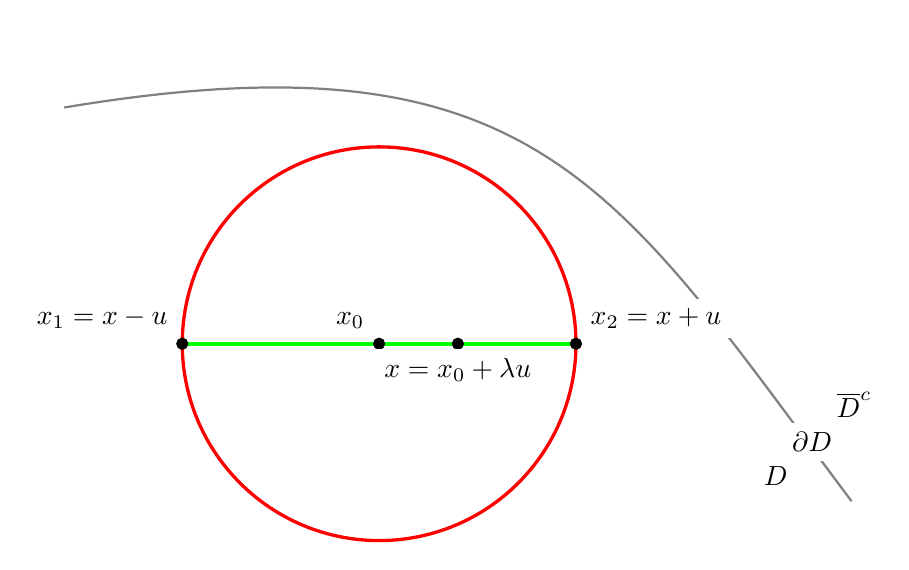
\begin{tikzpicture}
    \draw[gray, thick] (0, 5) .. controls (6, 6) and (7, 4) .. (10, 0);
    \draw[red, very thick] (4, 2) circle(2.5);
    \draw[green, ultra thick] (1.5, 2) -- (6.5, 2);
    \filldraw[black] (4, 2) circle(2pt);
    \node[above left=0pt of {(4, 2)}, outer sep=2pt, fill=white] {\( x_{0} \)};
    \filldraw[black] (5, 2) circle(2pt);
    \node[below =0pt of {(5, 2)}, outer sep=2pt, fill=white] {\(
    x=x_{0}+\lambda u \)};
    \filldraw[black] (1.5, 2) circle(2pt);
    \node[above left=0pt of {(1.5, 2)}, outer sep=2pt, fill=white] {\( x_{1}=x-u \)};
    \filldraw[black] (6.5, 2) circle(2pt);
    \node[above right=0pt of {(6.5, 2)}, outer sep=2pt, fill=white] {\(
    x_{2}=x+u \)};
    \node[above right=5pt of {(9.5, 0.75)}, outer sep=2pt, fill=white] {\( 
    \overline{D}^{c}\)};
    \node[below left=5pt of {(9.5, 0.75)}, outer sep=2pt, fill=white] {\(
    D\)};
    \node[, outer sep=2pt, fill=white] at (9.5, 0.75) {\(
    \partial D\)};
  \end{tikzpicture}

  Let \( u = x - x_{1} \), then \( x_{1} = x - u \), \( x_{2} = x+ u \) and
  there exists some \( \lambda > 0 \) such that \( x = x_{0} + \lambda u \).

  Then, we have
  \begin{align*}
    x = x_{0} + \lambda u = x_{0} + \lambda (x_{2} - x_{0}) = \lambda x_{2} + (1
    - \lambda) x_{0}\\
    \implies f(x) \le \lambda f(x_{2}) + (1- \lambda) f(x_{0})
  .\end{align*}, and
  \begin{align*}
    x &= x_{0} + \lambda u = x_{0} + \lambda ( x_{0} - x_{1}) \\
    &\implies x_{0} = \frac{1}{\lambda + 1} x + \frac{\lambda}{\lambda + 1}
    x_{1}\\
    &\implies f(x_{0}) \le  \frac{1}{\lambda + 1} f(x) + \frac{\lambda}{\lambda +
    1} f(x_{1})
  .\end{align*}

  Let \( M = \sup_{x \in \partial B(x, \varepsilon)} f(x) \) , then \( M \ge
  f(x_{1}), f(x_{2}) \) and \( f(x) \le  \lambda M + (1-\lambda)f(x_{0}) \) and
  \( f(x_{0}) \le \frac{1}{\lambda+1} f(x) + \frac{\lambda}{\lambda+1} M \).
  Another thing to note is that \( M \) is finite due to \( f \) not yielding
  any infinities.

  Hence, we have the following inequalities:

  \begin{align*}
    f(x) - f(x_{0}) &\le  \lambda(M - f(x_{0}))\\
    f(x) + \lambda M &\ge (\lambda + 1) f(x_{0})\\
    \implies f(x) - f(x_{0}) &\ge  \lambda (f(x_{0}) - M)
  .\end{align*}

  Hence, \( 0 \le  |f(x) - f(x_{0})| \le  \lambda (M-f(x_{0})) \), and let \( x \to
  x_{0} \), then \( \lambda \to  0 \) and therefore by the squeeze theorem, \(
  f(x) \to  f(x_{0}) \). Therefore \( f \) is continuous at \( x_{0} \).
\end{proof}

\begin{theorem}
  Let \( f \) be a function on open convex set \( D \).

  If \( f \) is convex, then for all directions \( d \neq  0 \),
  \( \frac{\partial f}{\partial d}(x_{0})  \), the
  \textbf{directional derivative} of \( f \) at \( x_{0} \in D \) wrt direction
  \( d \) exists and satisfies \( \frac{\partial f}{\partial d} (x_{0}) \le f(x_{0} + d) -
  f(x_{0}) \) if \( x_{0} + d \in D \).

  If \( f \) is differentiable, \( \nabla f = f'^{T} \) is the \textbf{gradient}
  of \( f \) exists. Then \( f \) is convex iff \( f(y)-f(x) \ge f'(x)(y-x)
   = \langle \nabla f(x), y -x\rangle\) for all \( x,y\in D \). Moreover, \( f
   \) is strictly convex on \( D \) iff equality only holds if \( x = y \).
\end{theorem}

\begin{proof}
  Consider the scalar function \( g(t) = f(x_{0}+t d) \), then \( g \) is
  defined on some neighborhood \( B(0, \varepsilon) \) of \( 0 \).

  We will prove that \( g \) is convex. This is true since \( g(\mathcal{C}(T,
  \lambda)) = f(x_{0} + \mathcal{C}(T, \lambda)d) = f(\mathcal{C}(x_{0} + Td,
  \lambda) \), because of linearity. Since \( f \) is convex \( g(\mathcal{C}(T,
  \lambda)) = f(\mathcal{C}(x_{0}+Td, \lambda)) \le \mathcal{C}(f(x_{0}+Td),
  \lambda) = \mathcal{C}(g(T), \lambda) \), QED.

  Then, we just need to prove that \( g \) has right derivative at \( 0 \). This
  is indeed true, as for any \( 0 < u < v < \varepsilon \), if let \( \lambda =
  \frac{u}{v}\), then \( u = \lambda v + (1 - \lambda) 0 \) and \( g(u) \le
  \lambda g(v) + (1- \lambda)g(0) = \lambda g(v) + (1 - \lambda)g(0) \). Hence,
  \( \frac{g(u) - g(0)}{u} \le  \frac{g(v) - g(0)}{v} \), and the function
  \( h(x) = \frac{g(x) - g(0)}{x} \) is decreasing as \( x \to  0^{+} \). Hence,
  there is a limit \( L = \lim_{x \to 0^{+}} h(x)  \), which is the right
  derivative of \( g(x) \) at \( 0 \). Note that this derivative can be
  (negative) infinity, for example if \( g(x) = -\sqrt[3]{x}  \).

  In the case that \( x_{0} + d \in D \), \( h(1) \) is defined as \( h(1) =
  g(x_{0}  + d) - g(x_{0}) \ge  L = \frac{\partial f}{\partial d}(x_{0})  \), QED.

  Letting \( d = y - x \), then using the identity \( \frac{\partial f}{\partial
  d} (x_{0}) = f'(x_{0})d \) for differentiable \( f \), we have \( f(y)-f(x)
  \ge f'(x)(y-x) \) for all \( x, y \in D \) if \( f \) is convex.

  To prove the reverse direction, let \( x = \mathcal{L}(y, z, w) \) such that \(
  w \in [0, 1]\) (denoting \( \mathcal{L}(x, y, w) = wx + (1-w)y \) as the
  \textbf{linear interpolation} (lerp) from \( x \) to \( y \) with weight \( w \)).
  Then, \( f(z)-f(x) \ge f'(x)(z-x) \) and \( f(y)-f(x) \ge f'(x)(y-x) \).
  Lerping the two inequality: \( \mathcal{L}(f(y)-f(x),f(z)-f(x),w) \ge
  f'(x)\mathcal{L}(y-x, z-x, w) \), yields \( \mathcal{L}(f(y), f(z), w) - f(x)
  \ge  f'(x)(\mathcal{L}(y,z,w)-x\). RHS is \( 0 \) since \( x =
  \mathcal{L}(y,z,w) \), which means \( \mathcal{L}(f(y), f(z), w) \ge
  f(\mathcal{L}(y,z,w) \), which implies that \( f \) is convex.

  To prove the theorem in the strictly convex case, we can trivially use the
  above proof with some obvious modifications.
\end{proof}

Now, consider \( f: D \subseteq \mathbb{R}^{n} \to  \mathbb{R} \), then \(
\nabla f: D \subseteq \mathbb{R}^{n} \to  \mathbb{R}^{n} \), which is a vector
function. Hence, one can define the Jacobian of this function \( (\nabla f)' \).
This matrix, if it exists, is called the \textbf{Hessian} of \( f \). And in
most cases, it's symmetric, hence it could be written as \( (\nabla f)'^{T} =
\nabla ^2 f \). Then, one have the Taylor theorem: for a
twice-continuously-differentiable function \( f \) and \( x_{0}, \Delta x \)
such that \( x_{0}, x_{0} + \Delta x \in \operatorname{dom} f \), then there
exists some \( \theta \in [0, 1] \) such that:

\begin{align*}
  f(x_{0}+\Delta x) &= f(x_{0}) + f'(x_{0})\Delta x + \frac{1}{2} \Delta x^{T}
  \nabla ^2f(x_{0} + \theta \Delta x) \Delta x\\
&= f(x_{0}) + f'(x_{0})\Delta x + \frac{1}{2} \Delta x^{T}
  \nabla ^2f(x_{0}) \Delta x + o(\|\Delta x\|^2)
.\end{align*}

Using this theorem, one can prove the following important result, which can be
used to identify convex functions.

\begin{theorem}[Second derivative test for convex functions]
  Let \( f \) be a twice-continuously-differentiable function on an open convex
  domain \( D \). Then, \( f \) is convex iff \( \nabla ^2 f(x) \) is
  positive semi-definite. Moreover, \( f \) is strictly convex if \( \nabla ^2
  f(x) \) is positive definite.
\end{theorem}

\begin{proof}
  Rewrite Taylor theorem as
  \[
    f(x_{0}+\lambda d)-f(x_{0})-\lambda f'(x_{0})d =\lambda^{2}
    \frac{d^{T}\nabla^{2}f(x_{0} + t\lambda d)d}{2}
  .\], then \( f \) is convex iff LHS is non-negative for all \( x_{0}, \lambda
  \) and \( d \). Hence, if \( \nabla ^2 f \) is positive semi-definite, then
  RHS is non-negative and we have QED.

  If \( f \) is convex, then we use the other variant of the Taylor's theorem
  and have RHS equals to \( \frac{1}{2}\lambda ^2 d^{T}\nabla ^2 f(x_{0})d +
  o(\lambda ^2) \), which is dominated by the first term. Hence, \( \nabla ^2
  f(x_{0}) \) needs to be positive semi-definite for all \( x_{0} \in D \).

  The strictly convex case could be similarly proven.
\end{proof}

After all of that theory about convex functions, we have the following theorem,
which states a valuable property about convex minimization problems.

\begin{theorem}
  Consider the minimization problem \( P: \min f(x), x \in D \), with \( D \) being
  a convex set, \( f(x) \) convex on \( D \). Then, if \( P \) has a LOS \(
  x_{0} \), then \( x_{0} \) is also a GOS. Moreover, if \( f \) is strictly
  convex, then \( x_{0} \) is the SGOS of \( P \).
\end{theorem}

\begin{proof}
  Let \( x_{0} \) be a \( B(x_{0}, \varepsilon) \)-optimal solution of \( P \).

  Then for any \( x \in D \) that is more optimal than \( x_{0} \),
  any convex combination of \( x_{0} \) and \( x \) would be more optimal than
  \( x_{0} \). We will prove that there is one such combination \( x' =
  \mathcal{L}(x_{0}, x, w) \in B(x_{0}, \varepsilon) \setminus \{x_{0}\}   \).

  We can easily prove that \( d(x_{0}, x') = \|x'-x_{0}| = w|x-x_{0}| \), which
  can be arbitrary small (but still positive)
  s.t. \( w > 0 \), which means that one can always pick
  some \( w \) such that \( x' \in B(x_{0}, \varepsilon) \) and \( x' \) is more
  optimal than \( x_{0} \). Hence, there is no \( x \in D \) that is more
  optimal than \( x_{0} \).

  If \( f \) is strictly convex, then any convex combination of \( x_{0} \) with
  an \( x \neq  x_{0}  \) that is at least as optimal as \( x_{0} \)
  would be more optimal than both \( x \) and \( x_{0} \). Hence, such \( x \)
  could not exist, and \( x_{0} \) is the SGOS of the problem.
\end{proof}

% subsection Convex optimization problem (end)

% section General optimization problem (end)

% chapter General optimization problem (end)

    \chapter{Linear programming} % (fold)
\label{sec:Linear programming}

\section{General, standard form and augmented form linear programs} % (fold)
\label{sec:General, standard form and augmented form linear programs}

The most general form of a linear program is the following optimization problem.

\begin{align*}
  \min\, &f(x) = cx\\
  \text{s.t.}\, & Ax\ge b, x \in \mathbb{R}^{n}
.\end{align*}, for matrices \( A \in \mathbb{R}^{m \times n}\), row vector
\(c \in \mathbb{R}^{ 1\times  n} \).

\( m, n \) are called as the \textbf{number of variables} and the \textbf{number
of constraints} of the problem, respectively.

e.g. $\min f(x)=5x_{1}-6x_{2}+3x_{3}$ s.t. $8x_{1}+6x_{2}+6x_{3}=5$, $3x_{1}-2x_{2}+7x_{3}\geq 7$ and $x_{1},x_{2},x_{3}\geq 0$ has

\renewcommand\arraystretch{1.3}

\[
  [A|b]=\mleft[
  \begin{array}{ccc|c}
8 & 6 & 6 & 5 \\
-8 & -6 & -6 & -5 \\
3 & -2 & 7 & 7 \\
1 &  &  & 0 \\
 & 1 &  & 0 \\
	 &  & 1 & 0 \\
   \end{array}
   \mright], c=\begin{bmatrix}
5 & -6 & 3
\end{bmatrix}
\] (omited entries are \( 0 \))

As one can see, general form linear programs can model many different types of
constraints, like regular inequalities, equalities, and non-negative
requirements.

However, we will focus on solving a restricted form of the general problem, and
provide one a method to convert from any arbitrary general problem to a
restricted problem.

\begin{definition}
  A \textbf{standard form linear program} (SFLP) is an optimization problem in the
  form:
  \begin{align*}
  \min\, &f(x) = cx\\
  \text{s.t.}\, & Ax\ge b, x \ge  0
  .\end{align*}

  An \textbf{augmented form linear program} (AFLP) is an optimization problem in the
  form:
  \begin{align*}
  \min\, &f(x) = cx\\
  \text{s.t.}\, & Ax=  b, x \ge  0
  .\end{align*}
\end{definition}

To convert from the augmented form of a linear program to the standard form, one
can use the duplication trick as the above example, or even better, introduce a
new variable for each constraint. Such variables are called \textbf{slack
variables}.

\begin{align*}
  z &= \begin{bmatrix} x \\ y \end{bmatrix} \in \mathbb{R}^{n + m}\\
  A' &= \begin{bmatrix} A & I_{m} \end{bmatrix} \in \mathbb{R}^{m \times (n +
  m)}\\
    Ax \ge b &\iff y = b - Ax \ge  0\\
     &\iff  z \ge 0 \text{ and } Az = b
.\end{align*}, and
\begin{align*}
  &c' = \begin{bmatrix} c & 0_{m} \end{bmatrix} \in \mathbb{R}^{n + m}\\
  \implies f(x) &= cx = c'z = g(z)
.\end{align*}

Hence, the SFLP is equivalent to the following AFLP

  \begin{align*}
  \min\, &g(z) = c'z\\
  \text{s.t.}\, & A'z=  b, z \ge  0
  .\end{align*}

Converting from a general linear program to an SFLP is not as straightforward.
For every unbounded variables \( x^{i} \), let \( x^{i} = y^{i} - z^{i} \) for
some non-negative \( y^{i}, z^{i} \)
Then, the general problem is equivalent to the following SFLP

\begin{align*}
  \min\,&g(x') = c'x'\\
  \text{s.t.}\,& A'x' \ge  b, x' \ge  0
.\end{align*}, with 
\begin{align*}
  x' &= \begin{bmatrix} y \\ z \end{bmatrix} \in \mathbb{R}^{2n}\\
  A' & = \begin{bmatrix} A & -A \end{bmatrix} \in \mathbb{R}^{m \times  2n}\\
  c' &= \begin{bmatrix} c & -c \end{bmatrix} \in \mathbb{R}^{1 \times  2n} 
.\end{align*}.

Of course, this is the general case. In practice, one would want to minimize the
number of constraints and variables to make thing much easier to handle, by
utilizing "prebounded" and "already-slack" variables in the problem.
% section General, standard form and augmented form linear programs (end)

\section{Convex polyhedra} % (fold)
\label{sec:Convex polyhedra}

\subsection{Hyperplanes and related theorems} % (fold)
\label{sub:Hyperplanes and related theorems}

Consider the feasible for the above problem: \( D = \{x, Ax\ge b\}   \). Then,
one can see that \( D \) is the intersection of sets \( H_{i}=\{x, A^{i}x \ge
b^{i}\}   \) for \( i \) ranging from \( 1 \) to \( m \).

Now, we will have some names for these sets.

\begin{definition}
  A \textbf{hyperplane} is a set \( H \) in the form of \( H = \{x, ax =
  \alpha\}   \). \( H \) splits the whole space into two open sets, which are
  called \textbf{open half-spaces}: \( H_{1} = \{x, ax > b\}   \) and \( H_{2}
  = {x, ax < b} \). There are also closed half spaces \( H_{3} = H_{1} \cup H =
  \{x, ax \ge  b\}  \) and \( H_{4} = H_{2} \cup  H = \{x, ax \le  b\}   \). The
  vector \( a^{T} \) is the \textbf{normal} of \( H \).

  Let \( S \subseteq \mathbb{R}^{n} \) and \( x_{0} \in S \). Then, a hyperplane
  \( H = \{x, ax = \alpha\}   \) is a \textbf{supporting hyperplane} of \( S \)
  at \( x_{0} \) iff \( x_{0} \in H \) and either \( S \subseteq H_{1} \) or \(
  S \subseteq H_{2}\), with \( H_{1}, H_{2} \) being the closed half-spaces
  bounded by \( H \).

  Let \( A, B \) be two subsets of \( \mathbb{R}^{n} \). Then, a hyperplane \( H
  \) \textbf{separates} \( A \) and \( B \) if and only if \( H \) splits the \(
  \mathbb{R}^{n}\) space into two closed half-spaces \( H_{1} \) and \( H_{2} \)
  such that \( A \subseteq H_{1} \) and \( B \subseteq H_{2} \).
\end{definition}

Before going on proving the important hyperplane theorems, we start with a
simple lemma.

\begin{theorem}
  Let \( S \) be a nonempty closed set in \( \mathbb{R}^{n} \). Then for every
  \( x_{0} \in S^{c} \), there exists some \( x_{1} \in S \) such that \(
  d(x_{0}, x_{1}) \le d(x_{0}, x), \forall x \in S \).
\end{theorem}

\begin{proof}
  Note that this is basically a minimization problem: \( \min f(x) = d(x_{0}, x), x \in
  S\), then we can use the theorems in the last chapter to prove that a GOS
  exist. We will use Theorem \ref{thr:coercive condition}, which requires \(
  f(x) \) to be (lower semi-)continuous and \( \lim_{x \to \infty} f(x) = +\infty \), which are both trivial to prove.
\end{proof}

\begin{theorem}[Hyperplane Separation Theorem (Closed set-point variant)]
\label{thr:hst-closed-pt}
  Let \( S \) be a nonempty, convex, closed set. Then for every \( x_{0} \in S^{c}
  \), there exists some hyperplane separating \( S \) and \( \{x_{0}\}   \).
\end{theorem}

\begin{proof}
  Let \( x_{1} \) be the closest point on \( S \) to \( x_{0} \), denote \( d =
  (x_{1}-x_{0})^{T}\).

  Then, we will prove that the hyperplane \( H = \{x, dx = dx_{1}\}   \) is a
  supporting hyperplane of \( S \). If this is true, then it's trivial that \( H
  \) separates \( S \) and \( \{x_{0}\}   \).

  Now, we have \( dx_{0}-dx_{1}=-d^{T}d < 0 \), which means that \( x_{1} \in
  H_{1} = \{dx < dx_{1}\}   \). Hence, we need to prove that \( S \subseteq
  H_{2} = \{dx \ge  dx_{1}\}   \), or \( x \in S \implies dx \ge  dx_{1} \).

  Assuming that there is some \( x_{2} \in S \) such that \( dx_{2} < dx_{1} \).
  Consider the lerp between \( x_{2} \) and \( x_{1} \): \( x(\lambda) =
  \operatorname{lerp}(x_{2}, x_{1}, \lambda) \), which must be in \( S \) for
  every \( \lambda \in [0, 1] \)
  \begin{align*}
    x(\lambda) - x_{0} &= \operatorname{lerp}(x_{2}, x_{1}, \lambda) -
    x_{0}\\
                       &= \operatorname{lerp}(x_{2}-x_{1}, 0, \lambda) + (x_{1}
                       - x_{0})\\
                       &= \lambda(x_{2}-x_{1}) + d^{T}\\
  .\end{align*}

  \begin{align*}
    \|x(\lambda)-x_{0}\|^2 &= (\lambda(x_{2}-x_{1}) + d^{T})^{T}(\lambda(x_{2}-x_{1})
    + d^{T})\\
                           &= \|d\|^2 + 2\lambda d(x_{2}-x_{1}) + \lambda
                           ^2\|x_{2}-x_{1}\|^2\\
                           &= \|x_{1}-x_{0}\|^2 + \lambda g(\lambda)
  .\end{align*},
  with \( g(\lambda) = 2d(x_{2}-x_{1}) + \lambda \|x_{2}-x_{1}\|^2 < 0 \) for
  small \( \lambda > 0 \), which means that \( \lambda g(\lambda) < 0 \) and
  therefore \( x(\lambda) \) is closer to \( x_{0} \) than \( x_{1} \), which is
  a contradiction.
\end{proof}

\textbf{Remark. } The hyperplane constructed above is a supporting hyperplane of
\( S \) at \( x_{1} \).

\begin{corollary}
  A closed convex set \( S \) is the intersection of the closed half-spaces that
  contains \( S \).
\end{corollary}

\begin{proof}
  If \( x \in S \), then every closed half-space that contains \( S \) contains
  \( x \).

  If \( x \in S^{c} \), then there exists a supporting hyperplane separating \(
  S\) and \( \{x\}   \), which means that \( x \) could not be in the close
  half-space that \( S \) is in.
\end{proof}


\begin{theorem}[Supporting Hyperplane Theorem]
  \label{thr:sht-boundary}
  Let \( S \) be a nonempty convex set and a point \( x_{0} \in \partial S \).
  Then, there exists a supporting hyperplane of \( S \) at \( x_{0} \).
\end{theorem}

\begin{proof}
  In every open ball \( B(x_{0}, \varepsilon_{n}) \), pick a point \( x_{n} \in
  B(x_{0}, \varepsilon_{n}) \cap  S^{c}\). Then, \( \lim_{n \to \infty} x_{n} =
  x_{0}\) if \( \varepsilon_{n} \to  0 \), which we will fix to \( \varepsilon_{n}
  = \frac{1}{n}\) for example.

  Using the previous theorem, there exists hyperplanes \( H_{n} \) separating \(
  S\) from \( \{x_{n}\}   \). Let the normal unit vector of \( H_{n} \) be \(
  d_{n} \), with the convention that \( d_{n}(x-x_{n}) \ge 0, \forall  x \in
  S \).

  Hence, \( d_{n} \) is a sequence on the compact set \( \partial B(0, 1) \),
  which means that there must be a convergent subsequence \( d_{i_{n}} \) that
  converges to \( d \).

  Since \( d_{n}(x-x_{n}) \ge 0 \) for all \( x \in S \), letting \( n = i_{m}
  \) and \( m \to  \infty \), we have \( d(x-x_{0}) \ge 0 \), and therefore \(
  H=\{x, d(x-x_{0})\ge 0\}   \) is a supporting hyperplane of \( S \).
\end{proof}

\begin{corollary}[Hyperplane Separation Theorem (Set-point variant)]
\label{cor:hst-set-pt}
  Let \( S \) be a nonempty convex set, then for every \( x \in
  (\operatorname{Int} S)^{c} \), there is a supporting hyperplane \( H \) that
  separates \( S \) and \( \{ x\}   \).
\end{corollary}

\begin{proof}
  If \( x \in \partial S \), the supporting hyperplane exists due to Theorem
  \ref{thr:sht-boundary}.

  If \( x \in \overline{S}^{c} \), then if \(\overline{S} \) is a convex set,
  there exists a supporting hyperplane of \( \overline{S} \) at \( x \), which
  is also a supporting hyperplane of \( S \) at \( x \), due to Theorem
  \ref{thr:hst-closed-pt}.

  To conclude, one would need to prove that \( \overline{S} \) is convex, using
  the following lemma.
  \begin{lemma}
    Let \( S \) be a convex set. Then \( \overline{S} \) is also a convex set.
  \end{lemma}

  \begin{proof}[Proof of lemma]
    Consider \( x \in \overline{S} \). If \( x \in S \), then there is a trivial
    sequence \( x_{n} = x \) that converges to \( x \). Otherwise, if \( x \in
    \partial S \), then every neighborhood \( B(x, \varepsilon_{n}) \) of \( x
    \) has at least some point in \( S \), which will be denoted as \( x_{n} \).
    Then, the sequence \( x_{n} \) converges to \( x \) if one let \(
    \varepsilon_{n} \to  0 \) as \( n \to  \infty \), for example \(
    \varepsilon_{n} = \frac{1}{n} \). Hence, for every \( x \in \overline{S} \),
    there is always a sequence \( x_{n} \in S \) that converges to \( x \).

    Consider a subset \( A \subseteq \overline{S} \), then there exists a
    sequence of sets \( A_{n} \) that converges to \( A \).

    Then, \( x_{n} = \mathcal{C}(A_{n}, \lambda) \to  \mathcal{C}(A, \lambda) =
    x\) because of linearity, as \( n \to  \infty \). Note that \( x_{n} \in S
    \) and we need to prove that \( x \in \overline{S} \), which is the reverse
    direction of what we've just proven above.

    If \( x \notin \overline{S} \), then there exists a neighborhood \( B(x,
    \varepsilon) \) of \( x \) that does not intersect \( \overline{S} \).
    However, that neighborhood must contain infinitely many points in the
    sequence \( x_{n} \), which is a contradiction.

    Hence, \( x \in \overline{S} \), and therefore \( \overline{S} \) closed
    under convex combination.
  \end{proof}
\end{proof}

Finally, we can prove the \textbf{Hyperplane separation theorem}.
\begin{theorem}[Hyperplane Separation Theorem]
  Let \( A, B \) be nonempty disjoint convex sets, then there exists a
  hyperplane that separates the sets.
\end{theorem}

\begin{proof}
  Consider the set \( S = S_{1} - S_{2} = \{s_{1} - s_{2},
  s_{1} \in S_{1}, s_{2} \in S_{2}\}   \).

  \( S \) is convex, since if \( x_{1}-x_{2}, y_{1}-y_{2} \in S_{1}-S_{2} \)
  (s.t. \( x_{1},y_{1} \in S_{1}, x_{2}, y_{2} \in S_{2} \)), then a convex
  combination of the two, which can be written as \(
  \operatorname{lerp}(x_{1}-x_{2},y_{1}-y_{2},\lambda) =
  \operatorname{lerp}(x_{1},y_{1},\lambda) -
  \operatorname{lerp}(x_{2},y_{2},\lambda) \in S_{1}-S_{2} \) due to the fact
  that \( operatorname{lerp}(x_{i},y_{i}, \lambda) \in S_{i} \).

  Then, using Corollary \ref{cor:hst-set-pt}, there is a hyperplane separating
  \( S_{1}-S_{2} \) and \( \{0\}   \). Moreover, there is one such hyperplane
  that passes through \( 0 \), which could be constructed by slightly modifying
  the proofs of the above theorems. Denote this hyperplane as \( H = \{x, dx \ge
  0\}   \), then we have \( dx_{1} \ge  dx_{2}, \forall x_{1} \in S_{1}, x_{2}
  \in S_{2} \).

  Let \( \alpha = \inf dS_{1}, \beta = \sup dS_{2} \), then we have \( dx_{1}
  \ge  \alpha \ge  \beta \ge dx_{2}, \forall x_{1} \in S_{1},x_{2} \in S_{2} \),
  which yields at least one separating hyperplane of \( S_{1} \) and \( S_{2}
  \): \( H'(\gamma) = \{ dx = \gamma\}   \) for any \( \gamma \in [\alpha,\beta]
  \), which is a nonempty interval.
\end{proof}

% subsection Hyperplanes and related theorems (end)

\subsection{Extreme points and recession directions} % (fold)
\label{sub:Extreme points and recession directions}

\begin{definition}
  Let \( S \) be a subset of \( \mathbb{R}^{n} \).

  If \( S \) is convex, then \( x \in S \) is an \textbf{extreme point} if and only if
  it could not be written as a strictly convex combination of a collection
  of points in
  \( S \) not containing \( x \). In other words, \( x \in S \) is an extreme
  point if for every \( y, z \in S \setminus \{x\}, w \in (0, 1)   \), we have
  \( x \neq \operatorname{lerp}(y,z,w) \).

  If a vector \( v \) satisfies, \( x + tv \in S \) for every \( x \in S \), \(
  t \ge  0\), then \( v \) is a \textbf{recession direction} of \( S \).

  A recession direction \( v \) is called a \textbf{extreme direction} if it is
  not a strictly convex combination of any collection of recession directions
  not containing directions in the form \( kv \) for scalars \( k \in \mathbb{R}
  \).
\end{definition}

Now, we will prove a very important result of extreme points and its compact
convex set: the \textbf{Krein-Milman Theorem}. But before proving the whole
theorem, we will look at a lemma about \textbf{faces}.

\begin{lemma}
  Let \( S \) be convex compact set on \( \mathbb{R}^{n} \). Then a \textbf{face}
  \( F \)
  of \( S \) is a subset \( F \subseteq S \) such that if \( z =
  \operatorname{lerp}(x, y, w) \in F \) for some \( x, y \in S, 0 < w < 1 \),
  then \( x, y \in F\).

  Let \( c \) be a row vector, then the set \( F_{c}(S) = \operatorname{Argmax}
  \{cx, x \in S\}     \) is a face.

  An extreme point of a face \( F \) of \( S \) is also an extreme point of \( S
  \).
\end{lemma}

\begin{proof}
  If \( x = \operatorname{lerp}(y,z, w) \in F_{c} \) for some \( y,z \in S \),
  then \( cx = \operatorname{lerp}(cy, cz, w) \le \max \{cy, cz\}   \), which
  means that either \( y \) or \( z \) is a GOS of the problem. WLOG assuming \(
  cx = cy\), then we end up having \( cz = cx \). Therefore, \( y, z \in F_{c}
  \), and \( F_{c} \) is a face of \( S \).

  To prove the second statement, let \( x \) be an extreme point of \( F \).
  Assuming that there exists \( y, z \in S, \lambda \in (0, 1) \) such that \( x =
  \operatorname{lerp}(y, z, \lambda) \), then \( y, z \in F \) because of the
  definition of faces, which leads to a contradiction.
\end{proof}

\begin{theorem}[Krein-Milman Theorem (Existence)]
  Let \( S \) be a nonempty, compact and convex set. Then, \( S \) has at least
  one extreme point.
\end{theorem}

\begin{proof}
Denote \( S_{1} = S \). Then for every \( i \), assuming \( S_{i} \) is a
nonempty face (induction hypothesis). There will be some cases
\begin{itemize}
  \item If \( |S_{i}| = 1 \) and \( S_{i} = \{ s\}   \), then \( s \) is an
    extreme point of \( S \).
  \item If \( |S_{i}| \ge  2 \), then pick \( x, y \in S_{i}, x \neq y \). Then,
    consider the hyperplane \( H: ax = \alpha \) separating \( x \) and \( y \),
    i.e. \( ax < \alpha < ay \), which always exist. Then, let \( S_{i+1}
    \coloneqq F_{a}(S_{i}) \subset S_{i} \), which is a nonempty face that is a
    proper subset of \( S_{i} \) (since \( x \notin F_{a} \)).
\end{itemize}

Consider the family \( \mathcal{A} \) of all nonempty faces of \( S \), with the partial
order \( \subseteq \). Then, the above procedure will have to halt at some
point (Zorn's lemma).
\end{proof}

\begin{theorem}[Krein-Milman Theorem]
  Let \( S \) be a nonempty, compact and convex set. Then, \( S \) is the convex
  hull of \( E(S) \), the set of its extreme points.
\end{theorem}

\begin{proof}
  Using the previous theorem, one can see that \( E(S) \) is nonempty.
  Let \( T \) be the convex hull of \( E(S) \), then one can trivially
  see that \( T \subseteq S \). Assuming there exists \( x \in T \setminus S \),
  then by the Hyperplane Separation Theorem, there is a row vector \( a \) such
  that \( \sup aT < ax \).

  Consider the face \( F_{a} = \operatorname{Argmax} \{ ax, x \in S \}   \),
  then \( T \cap  F_{a} = \varnothing \). Then, the face \( F_{a} \) would have
  an extreme point \( e' \), which means that \( e'  \notin E(S)\), which is a
  contradiction.
\end{proof}

% subsection Extreme points and recession directions (end)

\subsection{Convex polyhedra} % (fold)
\label{sub:Convex polyhedra}

\begin{definition}
  A \textbf{convex polyhedron} (plural \textit{convex polyhedra}) \( P \) is
  the intersection of finitely many closed half-spaces.

  A \textbf{convex polytope} is a bounded convex polyhedron.
\end{definition}

Then, one can write \( P \) as \( P = \{x, Ax \ge  b\}   \) for some matrix \( A
\) and row vector \( b \), with the closed half-spaces defining \( P \) being
the half-spaces \( H_{i}: A^{i}x \ge  b^{i} \).

Now, we will prove the following theorem.

\begin{theorem}[Minkowski's Theorem for Polyhedra]
  Denote \( \operatorname{conv} V \) as the convex hull of \( V \) and \(
  \operatorname{cone} R \) as the conic hull of \( R \).

  Let \( P \) be a convex polyhedron, then \( P \subseteq \operatorname{conv} E(P) +
  \operatorname{cone} R(P)\), with \( E(P), R(P) \) denoting the set of all
  extreme points and extreme directions of \( P \), respectively.
\end{theorem}

\begin{proof}

\( P \subseteq \operatorname{conv} E(P) + \operatorname{cone} R(P) \) is equivalent to
the fact that \( \forall x\in P, x = e_{i}\lambda^{i} + r _{j}\mu ^{j} =
e\lambda + r\mu \), with \( e \) and \( r \) being matrices with columns being
extreme points and extreme directions of \( P \), respectively. The condition
for the vectors \( \mu  \) and \( \lambda \) are \( \mu  \ge 0 \) and \(
\sum_{i} \lambda_{i} = 1 \)

Now, let
\begin{align*}
  x' &= \begin{bmatrix} x \\ 1 \end{bmatrix} \\
  A' &= \begin{bmatrix} A & -b \end{bmatrix} 
.\end{align*},
then \( Ax \ge b \) only if \( A'x' \ge  0 \).

Consider the convex cone \( C = \{x', A'x' \ge  0\}   \). If one can
prove the theorem for \( C \), which has no non-zero extreme points, then \(
\forall x' \in C, x' = r'\mu' \).

Observes that there are two types of extreme direction in \( D \), one with the
\( (n+1) \)-th component being \( 0 \) and one with that component being a
positive value, which could be normalized to \( 1 \) without loss of generality. Then, split \( r' \) according to this categorization, \( v \) is the matrix
that contains all extreme directions of the first type and \( u \) containing
extreme directions of the second type.

Then, there exists \( \lambda, \nu \ge 0 \) such that \( x' = u\lambda + v\nu \).
Moreover, \( 1 = x'^{n+1} = u^{n+1}\lambda= \sum_{i} \lambda^{i} \) since \(
u^{n+1}_{i} = 1 \) for all \( i \), since the extreme directions of the second
type is already normalized (wrt its last component).

Now, denote \( U = u^{1..n}, V = v^{1..n} \), we have \( x = x'^{1..n} =
U\lambda+V\nu \). This suggests that \( U \) and \( V \)'s columns are
extreme points and extreme directions of \( P\), respectively. This can be
trivially proven as follows
\begin{align*}
  0 \le  A'u_{i} = \begin{bmatrix} A & -b \end{bmatrix}  \begin{bmatrix} U_{i}
\\ 1 \end{bmatrix}  = AU - b
.\end{align*}
Hence, \( U \in P \). If \( U \) is a strict convex combination of two other \(
X_{1}, X_{2} \in P\), then \( u \) is a strict convex combination (wrt the same
weight) of the two extreme directions of \( C \) \( x_{1}, x_{2} \) given by:
\begin{align*}
  x_{i} = \begin{bmatrix} X_{i} \\ 1 \end{bmatrix}, i \in \{1, 2\}  
.\end{align*}, which is a contradiction to the fact that \( u \) is an extreme
direction of \( C \).
\begin{align*}
  0 \le  A'v_{i} = \begin{bmatrix} A & -b \end{bmatrix} \begin{bmatrix} V_{i} 0
\end{bmatrix}  = AV_{i}
.\end{align*}

Hence, \( V_{i} \) is a recession direction of \( P \) due to the fact that \(
\forall x \in P, t \ge  0, A(x+tV_{i}) = Ax + tAV_{i} = Ax \ge  b \). Using the
same logic as above, we can prove that \( V_{i} \) is an extreme direction of \(
P\).

\end{proof}

Therefore, the proof would be completed if we have proven the theorem for the
convex cone case:

\begin{theorem}[Minkowski's Theorem for Cones]
  Let \( C = \{x, Ax \ge  0\}   \) be a polyhedral cone, then \( C \) is
  contained in the conic hull of \( R(C) \), the set of its extreme directions.
\end{theorem}

\begin{proof}
  First, we prove that the set \( C_{1} = \{ x, \exists \lambda \ge 0, x =
  R\lambda\}   \) is a polyhedral cone, since one can use the
  \textbf{Fourier-Motzkin elimination algorithm} to turn from \( x = R\lambda,
  \lambda \ge 0 \) to \( Ax \le  0 \), which is the inequality for a polyhedral
  cone.

  Then, we say that \( (A, R) \) is a \textit{double description pair} (DDP) if
  \( Ax \le  0 \iff \exists \lambda \ge 0, x = R\lambda  \). Then, we will
  proceed to prove that \( (R^{T}, A^{T}) \) is also a DDP.

  \begin{align*}
    &R^{T}y \le 0\\
    &\iff \lambda^{T} R^{T} y \ge 0, \forall  \lambda \ge 0\\
    &\iff (R\lambda)^{T} y \ge 0, \forall  \lambda \ge 0\\
  .\end{align*}

  Let \( x = R\lambda \), then \( R^{T}y \le 0 \) iff \( x^{T}y \ge 0, \forall
  \lambda \ge 0, x = R\lambda \), or equivalently \( Ax \le  0 \). Then, the
  last statement is equivalent to \( Ax \le  0 \implies x^{T}y \le  0 \)

  To conclude this proof, we need to use \textbf{Farkas' Lemma}.

  \begin{lemma}[Farkas' Lemma]
  \label{farkas}
    \( ax \ge  0, \forall  x \) s.t. \( Ax \ge  0 \) iff \( a = yA \) for some
    row vector \( y \ge  0 \)
  \end{lemma}

  \begin{proof}[Proof of Farkas' lemma]
    If \( a = yA \), then \( ax = yAx \ge  0, \forall  Ax \ge 0 \).

    If \( ax \ge  0, \forall Ax \ge 0 \) and \( a \neq  yA, \forall  y\ge 0 \),
    then consider the set \( S = \{yA, y \ge 0\}   \). Since \( a \notin S \)
    and \( S \) is closed, using Theorem \ref{thr:hst-closed-pt}, there is a
    hyperplane \( H \) strictly separating \( S^{T} \) and \( \{ a^{T}\}   \).
    Assuming \( H = \{t, x^{T}t \ge  \alpha\}   \) satisfies \( ax  <  \alpha
    \le   \inf Sx \). Note that \( 0 \in Sx \), then \( \alpha \) must be
    non-positive. If \( \alpha < 0 \) and the hyperplane \( H' = \{ t, x^{T}t =
    0\}   \) could not separate the two sets, then there exists some \( t \in S
    \) such that \( tx < 0 \). Then, there exists \( k > 0 \) such that \( t(kx)
    < \alpha\), with \( kx \in S \), which means the original hyperplane also could
    not separate the two sets, which is a contradiction. Hence, the hyperplane
    \( H' \) could separate the two set, i.e. \( ax < 0 \le \inf Sx \). Then,
    we have \( A_{i}x \ge  0 \) for all \( i \), since \( A_{i} =
    A\mathbf{e_{i}} \in S \), with \( \mathbf{e_{i}} \) denoting the \( i \)-th
    standard basis vector, and hence \( Ax \ge 0 \). To conclude, \( ax < 0 \)
    for some \( x \) s.t. \( Ax \ge 0 \), which is another contradiction.
  \end{proof}

Continuing with the proof, we have
\begin{align*}
  &(Ax \le 0 \implies x^{T}y \le 0)\\
  &\iff(Az \ge  0 \implies z^{T}y \ge  0) \text{ (letting \( z = -x \))}\\
  &\iff \exists \lambda \ge 0,  y = \lambda A\\
  &\iff \exists  \lambda' = \lambda^{T} \ge 0, y^{T} = A^{T}\lambda'
.\end{align*}

Hence \( (R^{T}, A^{T}) \) is a DDP.

So to find \( R \), one find do Fourier-Motzkin on \( A^{T} \) to get \( R^{T}
\). Now that \( R \) exists, we have \( C = \{x, Ax \ge 0\} = \{x, \exists
\lambda \ge 0, x = -R\lambda\}  \)

Now, we will prove that \( -R_{i} \) are recession directions of \( C \).
Since \( R_{i} = R\mathbf{e_{i}}, \mathbf{e_{i}} \ge 0 \), \( R_{i} \in P \),
and \( AR_{i} \ge  0 \). Then, for every \( x \in P, t \ge 0 \), we have \( A(x
- tR_{i}) = Ax - tAR_{i} \le  0 \), which means that \( R_{i} \) is a recession
direction of \( C \). Pick columns from \( R \) to form a conical basis of \( R \)'s
column space, then this basis is able to span the recession cone of \( C \), due
to every recession direction \( d \) of \( C \) can be written as \( d =
R\lambda = R'\lambda' \) with some \( \lambda, \lambda' \ge  0 \).
\end{proof}

% subsection Convex polyhedra (end)

% section Convex polyhedra (end)

\section{Existence and properties of solutions of linear programs} % (fold)
\label{sec:Existence and properties of solutions of linear programs}

Firstly, since \( D = \{x\ge 0, Ax \ge  b\}   \) is a convex set (this can be
trivially seen due to the linearity of the convex combination operation) and \(
f(x)=cx\) is a convex (and a concave) function on \( \mathbb{R}^{n} \), then
every (S)LOS of the linear program is a (S)GOS.

The set \( D \) is already closed (why?) and \( f(x) \) is continuous, and hence
the problem will have a GOS if \( D \) is bounded.
% section Existence and properties of solutions of linear programs (end)

% chapter Linear programming (end)

    \chapter{Unconstrained Nonlinear Programming} % (fold)
\label{chap:Unconstrained Nonlinear Programming}

Consider the optimization problem:
\begin{align*}
  (P): \min\,&f(x),\\
  \text{s.t.}\,&x \in \mathbb{R}^{n}
,\end{align*} for \( f: \mathbb{R}^{n} \to \mathbb{R} \) is not a linear
(or affine) function.

Since \( x \) can freely take any value on \( \mathbb{R}^{n} \), this is an
unconstrained nonlinear program. However, if one makes changes to \( f \) that
makes \( f: \mathbb{R}^{n} \to \overline{\mathbb{R}}  \), this is generally
considered to be a constrained problem, since \( x \) effectively could not take
values that results in \( f(x) = +\infty \).

when \( f \) is convex, one would say that this is a convex program.
These programs have many interesting properties. One of such is the fact that
all LOSes of a convex program are GOSes. Here is another such property:

\section{A fresher on Multivariable Calculus} % (fold)
\label{sec:A fresher on Multivariable Calculus}

\subsection{Derivative and related concepts} % (fold)
\label{sub:Derivative and related concepts}

Here is the definition of the derivative of a single variable function:
\begin{definition}[Derivative of single variable functions]
\label{def:Derivative of single variable functions}
  Let \( f: D \to  \mathbb{R} \), \( D \subseteq \mathbb{R} \). Then, if the
  limit
  \[
    L = \lim_{x \to x_{0}} \frac{f(x) - f(x_{0})}{x - x_{0}} = \lim_{h \to 0}
    \frac{f(x_{0} + h) - f(x_{0})}{h}
  \] exists, then \( L \) is called the derivative of \( f \) at \( x_{0} \).
  Then, we say that \( f \) is differentiable at \( x_{0} \).

  The derivative of a single variable function \( f \) is the function \( f' \)
  such that \( f'(x_{0}) \) is the derivative of \( f \) at \( x_{0} \), for all
  \( x_{0} \in D \) that \( f \) is differentiable at.
\end{definition}

Now, we will try to generalize this concept to multi variable functions, \( f:
\mathbb{R}^{n} \to  \mathbb{R}^{m} \). The problem here is the fact that when
one let \( x \) to be a vector, then \( x - x_{0} \) or \( h \) has became a
vector. and we can't divide by vectors. If one simply replace \( h \) by its
norm, the definition would no longer be compatible with the single variable
derivative, since the direction of \( d \) is disregarded in the limit.

An approach to resolving this problem is to consider the following:
\[
  L = \lim_{h \to 0} \frac{f(x_{0} + h) - f(x_{0})}{h} \iff \lim_{h \to 0}
  \left| \frac{f(x_{0} + h) - f(x_{0}) - Lh}{h} \right|  = 0
.\] 

Here, we can freely replace \( h \) in the denominator by \( \|h\| \), resulting
in the following definition of the derivative:
\begin{definition}[Fréchet derivative]
\label{def:Fréchet derivative}
  Let \( V \) and \( W \) be normed linear spaces (with norms \( \|\cdot\|_{V} \)
  and \( \|\cdot\|_{W} \) respectively) and \( f: U \to W \), \( U \subseteq V
  \). Then for \( x_{0} \in \operatorname{Int} U \), the derivative of \( f \)
  at \( x_{0} \) is the linear map \( L(x) \) such that:
  \[
    \lim_{\|h\|_{W} \to 0} \frac{\|f(x_{0} + h) - f(x_{0}) -
    L(h)\|_{W}}{\|h\|_{V}}  = 0
  .\] 

  If such linear map does not exist, then we say \( f \) is not differentiable
  at \( x_{0} \).
\end{definition}

Because of the generalized nature of the Fréchet derivative, we will simply call
it the multivariable derivative or the derivative.

\textbf{Example:} Prove that the derivative of \( x^{T}Ax \) at \( x_{0} \) is
the \( L(h) = x_{0}^{T}(A+ A^{T})h \) (\( x \in \mathbb{R}^{n}, A \in
\mathbb{R}^{n\times n} \))
\begin{proof} 
  We simply take this limit:
  \begin{align*}
    &\lim_{\|h\| \to 0} \frac{|(x_{0}+h)^{T}A(x_{0}+h) - x_{0}^{T}Ax_{0} -
    (x_{0}^{T}A + x_{0}A^{T})h|}{\|h\|}\\
    &= \lim_{\|h\| \to 0} \frac{|h^{T}Ah + (x_{0}^{T}Ah + h^{T}Ax_{0}) -
    (x_{0}^{T}Ah + x_{0}^{T}A^{T}h)|}{\|h\|}   \\
    &= \lim_{h \to  0} \frac{|h^{T}Ah|}{\|h\|} \\
  .\end{align*}
Note that here, \( x_{0}^{T}A^{T}h = \langle x_{0}, A^{T}h \rangle = (A^{T}h)^{T}x_{0} =
h^{T}Ax_{0} \). It suffices to show that the final limit, which is independent
of \( x_{0} \), converges to \( 0 \).

We have \( 0 \le  |h^{T}Ah| = |\langle h, Ah \rangle| \le \|h\| \|Ah\| \)
(Cauchy-Schwarz inequality). Hence, we simply need to prove \( \|Ah\| \to 0 \)
as \( \|h\| \to 0 \). In fact, we have the following stronger statement:

\begin{lemma}[Every linear map between Euclidean spaces are bounded]
\label{lem:Every linear map between Euclidean spaces are bounded}
  Every linear map \( L: \mathbb{R}^{n} \to  \mathbb{R}^{m} \) is bounded, i.e.
  there exists some \( M \) such that \( \|Lx\| \ge M\|x\| \).
\end{lemma}

\begin{proof}
  Let \( A \) be the matrix of the linear map (wrt standard basis), then \( L(x)
  = Ax\). Let \( X = \max \{|A^{i}_{j}|, i \in 1..m, j \in 1..n\}   \), then, \( (Ax)^{i}
  = A^{i}x = A^{i}_{j}x^{j} \) and \( |(Ax)^{i}| \le |A^{i}_{j}x^{j}| \le
  |A^{i}_{j}| |x^{j}| \le nX\|x\| \).

  Then, we have \( \|Ax\| \le m(nX\|x\|) = n^2X \|x\| \) and hence \( \|Ax\| \ge
  mnX \|x\|\).
\end{proof}

To finalize our proof of the example, note that since \( \frac{\|Ah\|}{\|h\|} \)
is bounded, as \( h \to 0 \), \( Ah \to 0 \).
\end{proof}

Much like the usual derivative, the multivariable derivative have many familiar
properties. One of them is uniqueness.

\begin{theorem}[Uniqueness of multivariable derivative]
\label{thr:Uniqueness of multivariable derivative}
  Let \( f: \mathbb{R}^{n} \to  \mathbb{R}^{m} \) be a function that is
  differentiable at \( x_{0} \). Moreover, let \( L_{1} \) and \( L_{2} \) be
  the multivariable derivative of \( f \) at \( x_{0} \). Then, \( L_{1} = L_{2}
  \).
\end{theorem}
\begin{proof}
  Fix some vector \( d \neq 0 \) and let \( h = t d \). WLOG, assuming \( \|d\|
  = 1\).

  Since \( L_{1} \) and \( L_{2} \) are both the derivative of \( f \) at \(
  x_{0} \), we have the following limits:
  \begin{align*}
    \lim_{t \to  0} \frac{\|f(x_{0} + t d) - f(x_{0}) - tL_{1}(d) \|}{|t|} &= 0\\
    \lim_{t \to  0} \frac{\|f(x_{0} + t d) - f(x_{0}) - tL_{2}(d) \|}{|t|} &= 0\\
  .\end{align*}

  Then, using the squeeze theorem for:
  \begin{gather*}
    0 \le \|L_{1}(d) - L_{2}(d)\| = \frac{\left\| (f(x_{0}+t d) -
    f(x_{0})-tL_{1}(d)) - (f(x_{0} + t d) - f(x_{0}) - tL_{2}(d) \right\|
  }{|t|}\\
  \le 
    \frac{\|f(x_{0} + t d) - f(x_{0}) - tL_{1}(d) \|}{|t|} +
    \frac{\|f(x_{0} + t d) - f(x_{0}) - tL_{2}(d) \|}{|t|} \to  0
  \end{gather*} as \( t \to 0 \), we have \( L_{1}(d) = L_{2}(d) \). Since this
  is true for all \( d \), we must have \( L_{1} = L_{2} \).
\end{proof}

Another instrumental property of multivariable derivative is the fact that
differentiability implies continuity.

\begin{theorem}[Differentiability implies continuity]
\label{thr:Differentiability implies continuity}
  If \( f \) is differentiable at \( x_{0} \), then \( f \) is continuous at \(
  x_{0}\).
\end{theorem}

\begin{proof}
  We have \( 0 = \lim_{h \to 0} \|f(x_{0} + h) - f(x_{0}) - L(h)\| \) or
  equivalently \( 0 = \lim_{h \to 0} (f(x_{0} + h) - f(x_{0}) - L(h)) \). Since
  \( L(h) \to 0 \) as \( h \to 0 \), we can factor out \( L(h) \) from the limit
  and we are left with \( \lim_{h\to 0} f(x_{0} + h) = f(x_{0}) \).
\end{proof}


Next, we will look at the multivariable chain rule.

\begin{theorem}[Multivariable chain rule]
\label{thr:Multivariable chain rule}
  Let \( f: X \subseteq \mathbb{R}^{n} \to  \mathbb{R}^{k}, g: Y \subseteq
  \mathbb{R}^{k} \to \mathbb{R}^{m} \) and some \( x_{0} \in \operatorname{Int}
  X\) such that there exists some neighborhood \( B(x_{0}, \varepsilon)
  \subseteq X \) that is mapped to a subset of \( Y \) by \( f \) (i.e. \(
  f(B(x_{0}, \varepsilon)) \subseteq Y \)).

  Then, denote \( g \circ f \) as the composition of two functions \( g \) and
  \( f \), i.e. the function \( (g \circ f)(x) = g(f(x)) \), \( Df(x_{0}) \) as
  the multivariable derivative of \( f \) at \( x_{0} \) (\( Df(x_{0})(h) \) is
  the value of that linear map for the direction \( h \)), if \( f \) is
  differentiable at \( x_{0} \) and \( g \) is differentiable at \( f(x_{0}) \),
  one can calculate the derivative of \( g \circ f \) as:
  \[
    D(g \circ f)(x_{0}) = Dg(f(x_{0})) \circ Df(x_{0})
  .\] 
\end{theorem}

\begin{proof}
  Denote \( u = g \circ f \), \( L_{f} = Df(x_{0}) \) and \( L_{g} = Dg(f(x_{0})
  \). Basically, we want to prove that \( Du(x_{0}) = L_{g} \circ  L_{f} \).

  Back to the definition, we have:
  \begin{align*}
    &0 \le  \frac{\|u(x_{0} + h) - u(x_{0}) - L_{g}(L_{f}(h))\|}{\|h\|}\\
    &\le  \frac{\left\| \left( g(f(x_{0} + h)) - g(f(x_{0})) -
    L_{g}(f(x_{0} + h) - f(x_{0})\right)  \right\| }{\|h\|} +
    \frac{\left\| L_{g}\left( f(x_{0} + h) - f(x_{0}) -
        L_{f}(h)
    \right)  \right\| }{\|h\|}
  .\end{align*}
  We will prove that both of these terms converges to \( 0 \) as \( \|h\| \to 0
  \).

  The second term trivially converges by the definition of the derivative:
  \[
    \lim_{h \to  0} \frac{\|f(x_{0} + h) - f(x_{0}) - L_{f}(h)\|}{\|h\|} = 0
  .\] 

  For the first term, denote \( x_{1} = f(x_{0}) \) and \( h_{1} = f(x_{0} + h)
  - f(x_{0})\). Then, the first term can be written in the form:
  \[
    \frac{\|g(x_{1} + h_{1}) - g(x_{1}) - L_{g}(h_{1})\|}{\|h_{1}\|} \cdot
    \frac{\|h_{1}\|}{\|h\|}
  .\]

  Since \( f \) is differentiable at \( x_{0} \), by Theorem
  \ref{thr:Differentiability implies continuity}, \( f \) is continuous at \( x_{0}
  \), and as \( h \to 0 \), \( h_{1} = f(x_{0} + h) - f(x_{0}) \to 0 \).

  Hence, the first factor converges to \( 0 \), by the definition of the
  derivative. Now, we will prove that \( \frac{\|h_{1}\|}{\|h\|} \) is bounded.

  We have:
  \[
    0 \le  \frac{\|h_{1}\|}{\|h\|} \le  \frac{\|f(x_{0}+h) - f(x_{0}) -
    L_{f}(h)\|}{\|h\|} + \frac{\|L_{f}(h)\|}{\|h\|}
  .\] 

  The first term converges to \( 0 \), and same for the second one by Lemma
  \ref{lem:Every linear map between Euclidean spaces are bounded}, we have what
  we needed.
\end{proof}

Now, since linear maps can be represented as matrices (in a specific basis, we
will only care about the standard basis here), we will look at the matrix
representing the multivariable derivative. That matrix is called the
\textbf{Jacobian matrix}.

We will be interested in calculating the Jacobian matrix. Denote the
multivariable derivative and the Jacobian
matrix of the function \( f \) at \( x_{0} \) as \( L \) and \(
f'(x_{0}) \), respectively, we have:
\[
  L(h) = f'(x_{0})h = f'(x_{0})_{i}h^{i}
.\] 

The idea now is to substitute \( h^{i} \) with special vectors in order to find
every column of \( f'(x_{0}) \). In particular, let \( h = \mathbf{e_{j}} \) for
some fixed \( j \), we have \( L(\mathbf{e_{j}}) =
f'(x_{0})_{i}\mathbf{e_{j}}^{i} = f'(x_{0})_{j} \).

Hence, one can write \( f'(x_{0}) \) as the following:
\[
  f'(x_{0}) = \begin{bmatrix} L(\mathbf{e_{1}}) & L(\mathbf{e_{2}}) & \ldots  &
  L(\mathbf{e_{n}})\end{bmatrix} 
.\] 

As one can see, the value of \( L \) at \( \mathbf{e_{j}} \) serves as some kind
of basis in some "derivative" space. Motivated by this, we have the following
definitions.

\begin{definition}[Directional and Partial derivative]
\label{def:Directional and Partial derivative}
  Let \( f: X \subseteq \mathbb{R}^{n} \to  \mathbb{R}^{m} \) and \( x_{0} \in
  X \). For a direction vector \( d \neq 0 \) satisfying \( [x_{0}-d,
  x_{0}+\varepsilon d]  \subseteq X  \), the \textbf{directional
  derivative} of \( f \) at \( x_{0} \) wrt directiion \( d \), denoted as
  \(\frac{\partial f}{\partial d}(x_{0})\), is defined as:
  \[
    \frac{\partial f}{\partial d}(x_{0}) = \lim_{t \to 0^{+}} \frac{f(x_{0}+t d)
    - f(x_{0})}{t } \text{ (if the limit exists)}
  .\]

  In particular, if \( d = \mathbf{e_{i}} \) is the \( i \)-th standard basis
  vector, this partial derivative is called the \textbf{partial derivative} of
  \( f \) at \( x_{0} \) wrt \( x^{i} \), denoted alternatively as \(
  \frac{\partial f}{\partial x^{i}} \).
\end{definition}

By this definition, we see that if the multivariable derivative \( L \) exists
at some \( x_{0} \) of the function \( f \), then:
\[
  \lim_{t \to 0^{+}} \frac{f(x_{0} + t d) - f(x_{0}) - tL(d)}{t \|d\|} = 0 
,\] which implies
\[
  L(d) = \lim_{t \to  0^{+}} \frac{f(x_{0} + t d) - f(x_{0})}{t} =
\frac{\partial f}{\partial d}(x_{0}) = f'(x_{0})d.\] 

Therefore, both directional derivatives and partial derivatives can be derived
from the multivariable derivative (or the Jacobian matrix), if it exists. Do
note that if the multivariable derivative does not exist, these quantities may
still exist, and one might have to compute them directly.

We still can now solve the problem of computing multivariable derivative (and
related quantities) by computing the Jacobian matrix, which depends on the \(
L(\mathbf{e_{i}}) \) vectors, which are the partial derivative wrt \( x^{i} \).
Note that we have \( f'(x_{0})_{i} = L(\mathbf{e_{i}}) \), so one can denote \(
f'_{i}(x_{0})\) or \( f'_{x^{i}}(x_{0}) \) as the partial derivative wrt \( x_{i} \) (this is simply a
notation, and it doesn't depend on whether the multivariable derivative exist or
not).

To calculate partial derivatives, note that all variables \( x^{j} \) with \( j
\neq  i\) seems to stay constant in the limit. Hence, one can simply treat them
as constants, and calculate the derivative of \( f(x) \) with only one variable.
If \( m \) is greater than \( 1 \), we simply calculate the derivative of each
component of \( f \) separately, and then put them all in a vector.
\[
  f'_{i}(x_{0})^{j} = (f^{j})_{i}'(x_{0})
.\] 

Here is an example to illustrate this:

\textbf{Example:} Find the mutlivariable derivative of \( f(x, y, z) =
\begin{bmatrix} xyz \\ e^{y} + x^2 \end{bmatrix}  \).

Calculating the partial derivatives yields:
\begin{alignat*}{2}
  f'^{1}_{x}(x, y, z) &= \frac{d}{dx}(xyz) &= yz\\
  f'^{1}_{y}(x, y, z) &= \frac{d}{dx}(xyz) &= xz\\
  f'^{1}_{z}(x, y, z) &= \frac{d}{dx}(xyz) &= xy\\
  f'^{2}_{x}(x, y, z) &= \frac{d}{dx}(e^{y}+x^2) &= 2x\\
  f'^{2}_{y}(x, y, z) &= \frac{d}{dy}(e^{y}+x^2) &= e^{y}\\
  f'^{2}_{x}(x, y, z) &= \frac{d}{dz}(e^{y}+x^2) &= 0\\
\end{alignat*}
Putting this all in the Jacobian matrix, we have:
\[
  f'(x, y, z) = \begin{bmatrix} yz & xz & xy \\ 2x & e^{y} & 0 \end{bmatrix} 
.\] 

Hence, one can write the mutlivariable derivative as:
\[
  L(x, y, z)(h) = \begin{bmatrix} yz & xz & xy \\ 2x & e^{y} & 0 \end{bmatrix} h
.\] 

We still have a problem, however. All of our results above relies on the fact
that \( f \) is differentiable, but there is no way to check that without having
to find the multivariable derivative. Of course, oone could always assume that
such derivative exists, and find it using partial derivatives and Jacobian
matrices, then substitute it into the definition and thus proving such
derivative exists, which is not convenient, to say the least. This theorem helps
with improving things up:

\begin{theorem}[Continuous partials implies differentiability]
\label{thr:Continuous partials implies differentiability}
  Let \( f: X \subseteq \mathbb{R}^{n} \to  \mathbb{R}^{m} \). If every partial
  derivatives
  of \( f \) is continuous in a neighborhood of \( x_{0} \in \operatorname{Int}
  X\), then \( f \) is
  differentiable at \( x_{0} \).
\end{theorem}

This theorem essentially were the "substitute the multivariable derivative back
to the definition to show such derivative exists" step above.

\begin{proof}
  First, since the components of \( f \) are independent, we may assume \( m = 1
  \). And since partial derivatives of \( f \) exists (and is continuous), we
  can construct the Jacobian matrix \( f'(x_{0}) \) of \( f \). Note that this
  is simply a notation, not proving \( f \) is differentiable at \( x_{0} \).

  Consider \( l(x_{0}, d) = f(x_{0} + d) - f(x_{0}) - f'(x_{0})d \). The idea
  here is to replace this by the sum of \( n \) expressions like \( l(x_{k},
  t\mathbf{e_{i}}) \), which "aligns" with partial derivatives.

  Define \( u_{k} = d^{k}\mathbf{e_{k}} \), then \( d = d^{k}\mathbf{e_{k}} =
  \sum_{k} u_{k} \). Denote \( x_{n} = x_{0} + d \), we have \( x_{n} = x_{0} +
  \sum_{k=1}^{n} u_{k}\). Recursively defining \( x_{i} = x_{i - 1} + u^{i} \)
  for \( i \in 1..n \), we have \( x_{n} = x_{0} + d \), and we have:

  \begin{align*}
    l(x_{0}, d) &= f(x_{n}) - f(x_{0}) - f'(x_{0})d \\
    &= \sum_{k = 1}^{n} (f(x_{k}) - f(x_{k-1}) - f'(x_{0})u_{k}) \\
    &= \sum_{k = 1}^{n} (f(x_{k-1} + u_{k}) - f(x_{k-1}) - f'(x_{0})u_{k}) \\
    &= \sum_{k = 1}^{n} l(x_{k-1}, u_{k})
  .\end{align*}

  Finally, we need to prove \( \lim_{d \to 0} \frac{\|l(x_{k-1},
  u_{k}\|)}{\|d\|} = 0  \) for every \( k \) (with \( x_{k-1} \) and \( u_{k} \)
  are both dependent on \( d \)). Since \( d \to 0 \), at some point \( x_{k-1}
  \) is in \( B(x_{0}, \varepsilon) \), the neighborhood of \( x_{0} \) such
  that partial derivatives of \( f \) are continuous. We have:
  \begin{align*}
    0 \le \frac{\|l(x_{k-1}, u_{k}\|)}{\|d\|} &= \frac{\|f(x_{k-1}+u_{k}\|)-f(x_{k-1})
    -f'(x_{k-1})u_{k}\|}{\|d\|} + \frac{\|f'(x_{k-1}) - f'(x_{0})\|
  \|u_{k}\|}{\|d\|} \\
&\le \frac{\|f(x_{k-1}+u_{k}\|)-f(x_{k-1})
    -f'(x_{k-1})u_{k}\|}{\|u_{k}\|} + \frac{\|f'(x_{k-1}) - f'(x_{0})\|
  \|u_{k}\|}{\|u_{k}\|} \to 0
,\end{align*} as \( u_{k} \to 0, x_{k-1} \to x_{0} \) when \( d \to 0 \). Using
the squeeze theorem, we have exactly what we needed. Here, the fact that partial
derivatives are continuous is used to show that \( f' \) is continuous.
\end{proof}

% subsection Derivative and related concepts (end)

\subsection{Definite matrices} % (fold)
\label{sub:Definite matrices}

\begin{definition}[Definiteness of matrices]
\label{def:Definiteness of matrices}
  A square matrix \( A \in \mathbb{R}^{n\times n} \) is:
  \begin{itemize}
  \item \textbf{Positive-definite}, if \( x^{T}Ax > 0 \) for every \( x \in
    \mathbb{R}^{n\times n}, x \neq 0 \).
  \item \textbf{Positive-definite}, if \( x^{T}Ax < 0 \) for every \( x \in
    \mathbb{R}^{n\times n}, x \neq 0 \).
  \item \textbf{Positive semi-definite}, if \( x^{T}Ax \ge 0 \) for every \( x \in
    \mathbb{R}^{n\times n} \).
  \item \textbf{Negative semi-definite}, if \( x^{T}Ax \le 0 \) for every \( x \in
    \mathbb{R}^{n\times n} \).
  \end{itemize}
\end{definition}

Since \( \mathbf{e_{i}}^{T}A\mathbf{e_{i}} = A^{i}_{i} \), one can simply look
at the diagonal to determine whether a matrix is *-definite or not. For
example, consider the following matrix:
\[
  A = \begin{bmatrix} 1 & 2 & 3 \\ 4 & 5 & 6 \\ 7 & 8 & -9 \end{bmatrix} 
.\] This matrix is neither in the four classes, since it has both negative and
positive entries on the diagonal.

\begin{theorem}[Skew-symmetric part does not affect definiteness]
\label{thr:Skew-symmetric part does not affect definiteness}
  For any square matrix \( A \), denote \( A' = \frac{A + A^{T}}{2} \) as the
  symmetric part of \( A \). Then, \( A \) is *-definite iff \( A' \) is
  definiteness, since:
  \[
    x^{T}Ax = x^{T}A'x
  ,\] for every vector \( x \in \mathbb{R}^{n} \).
\end{theorem}

\begin{proof}
  Since \( x^{T}Ax \) is a scalar, we have:
  \[
    x^{T}Ax = (x^{T}Ax)^{T} = x^{T}A^{T}x
  .\]

  Then, we have:
  \[
    x^{T}Ax = \frac{1}{2}(x^{T}Ax + x^{T}A'x) = x^{T}A'x
  .\] 
\end{proof}

Hence, if one want to check whether a non-symmetric part is *-definite or not,
one can use the criterions for symmetric matrix for the symmetric part of the
original matrix. Do note that, these criterions for symmetric matrices does not
work for non-symmetric ones.

In this part, we will introduce many results related to definite matrices and
especially checking if a given symmetric matrix \( A \) belongs to which type among the
four classes of matrices mentioned above (or whether it does not belong to any
of them). First, we have this important result:

\begin{theorem}[Eigenvalues of a definite matrix]
\label{thr:Eigenvalues of a definite matrix}
  Let \( A \in \mathbb{R}^{n\times n} \) be a symmetric matrix with \(
  \operatorname{Spec} A \) being the set of its eigenvalues. Then:
  \begin{itemize}
  \item \( A \) is positive-definite iff \( \operatorname{Spec} A \subseteq (0,
    +\infty) \).
  \item \( A \) is positive semi-definite iff \( \operatorname{Spec} A \subseteq [0,
    +\infty) \).
  \item \( A \) is negative-definite iff \( \operatorname{Spec} A \subseteq
    (-\infty, 0)\).
  \item \( A \) is negative semi-definite iff \( \operatorname{Spec} A \subseteq
    (-\infty, 0]\).
  \end{itemize}
\end{theorem}

\begin{proof}
  We will only prove this theorem for the first two cases. Since \( A \) is
  symmetric, there exists an eigendecomposition of \( A \), i.e. there exists an
  orthogonal matrix \( Q \) and a diagonal matrix \( D \) such that \( Q^{T} =
  Q^{-1} \) and \( A = QDQ^{-1} \).

  Then, \( x^{T}Ax = x^{T}QDQ^{T}x = \sum_{i} D^{i}_{i}((Q^{T}x)^{i})^2 \) (note
  that \( (\cdot)^2 \) here is the squaring operation, not a superscript). The
  values \( D_{i}^{i} \) here are the eigenvalues of \( A \), so if one of them
  is negative, i.e. \( D^{i}_{i} < 0 \) for some i, one can let \( Q^{T}x =
  \mathbf{e_{i}} \) and we have a negative result. Hence, if \( A \) is
  positive semi-definite, then \( D^{i}_{i} \ge 0 \) for all \( i \). For
  positive-definite, we have a similar result: \( D^{i}_{i} > 0 \) for all \( i
  \).

  In the reverse direction, we can see that if \( D^{i}_{i} > 0 \) (or \(
  D^{i}_{i} \ge 0 \)) for all \( i
  \), then the product is trivially positive (or non-negative).
\end{proof}

\begin{corollary}[Determinant and Trace of a definite matrix]
\label{cor:Determinant and Trace of a definite matrix}
  If \( A \) is a positive-definite, positive semi-definite, negative-definite
  or negative semi-definite matrix, then \( \det A \) and \( \operatorname{tr} A
  \) are both \( > 0 \), \( \ge 0 \),
  \( < 0 \) or \( \le 0 \) respectively.

  In the case \( n = 2 \), the signs of \( \det A \) and \( \operatorname{tr} A
  \) are sufficient to determine which type of definiteness a symmetric matrix
  \( A \) is.
\end{corollary}

\begin{proof}
  This trivially follows from the results:
  \begin{align*}
    \det A &= \sum_{\lambda \in \operatorname{Spec} A} \lambda\\
    \operatorname{tr} A &= \prod_{\lambda \in \operatorname{Spec} A} \lambda\\
  .\end{align*}

  When \( n = 2 \), we have \( \det A = \lambda_{1} + \lambda_{2} \) and \(
  \operatorname{tr} A = \lambda_{1}\lambda_{2} \). By considering multiple
  cases, one can trivially prove the latter part of the statement.
\end{proof}

To conclude, here is a very nice theorem about positive-definiteness.

\begin{theorem}[Sylvester's criterion]
\label{thr:Sylvester's criterion}
  Let \( A \in \mathbb{R}^{n\times n} \) be a symmetric matrix. Then, \( A \) is
  positive-definite if and only if \( \det A^{1..k}_{1..k} > 0 \) for all \( k
  \in 1..n \).
\end{theorem}

Despite its niceness, the proof of it involves many weird matrix decompositions
and is generally very long, complicated and most importantly, out of the scope
of what we are trying to learn here.

Note that this theorem only work for positive-definiteness (and
negative-definiteness if one negates the matrix). If one want to use
a similar result to check for positive semi-definite, one must consider the
determinants of all submatrices of \( A \), which is probably not worth it.

% subsection Definite matrices (end)

\subsection{Gradient and the Hessian matrix} % (fold)
\label{sub:Gradient and the Hessian matrix}

\begin{definition}[Gradient]
\label{def:Gradient}
  The gradient of a function \( f: X \subseteq R^{n} \to  \mathbb{R} \) at
  \( x_{0} \) is the transpose of the Jacobian matrix of \( f \) at \( x_{0} \),
  denoted as \( \nabla f(x_{0}) \).
\end{definition}

This definition suggests that Jacobian matrices are more "fundamental" than
gradients. Moreover, Jacobian matrices are more "general", in the sense that
they exist for functions \( f \) with \( m > 1 \), while the gradient (by
definition) does not.

However, \( \nabla f: \mathbb{R}^{n} \to  \mathbb{R}^{n} \), and this is
precisely a function that may have a derivative. Hence, to define the second
derivative, we have to rely on the gradient map. Here is the definition of the
second derivative:

\begin{definition}[Second derivative and the Hessian matrix]
\label{def:Second derivative and the Hessian matrix}
  Let \( f: X \subseteq \mathbb{R}^{n} \to \mathbb{R} \) and \( \nabla f \) be
  its gradient function. Then, if \( \nabla f \) is differentiable at some point
  \( x_{0} \in X \), then this derivative is called the \textbf{second
  derivative} of \( f \) at \( x_{0} \).

  The matrix of this second derivative linear map wrt the standard basis is
  called the \textbf{Hessian matrix} (or simply, the Hessian). This matrix is
  denoted as \( f''(x_{0}) = (\nabla f)'(x_{0}) \), or \( \nabla ^2f(x_{0}) \).
\end{definition}

To calculate the Hessian matrix, one simply calculate the (second-order) partial
derivatives:
\[
  f''(x_{0})^{i}_{j} = \frac{\partial}{\partial x_{j}} \left(
  \frac{\partial f}{\partial x_{i}} \right) = \frac{\partial ^2 f}{\partial
x_{j}\partial x_{i}}
.\] 

A very important properties of second-order partial derivatives:

\begin{theorem}[Symmetry of Second Derivatives]
\label{thr:Symmetry of Second Derivatives}
  (Also known as Schwarz's theorem, Clairaut's theorem or Young's theorem) Let
  \( f: X \subseteq \mathbb{R}^{n} \to  \mathbb{R} \), if \( x_{0} \in X \) and
  \( f''(x) \) exists and is continuous on some neighborhood of \( x_{0} \),
  then \( f''(x_{0}) \) is a symmetric matrix, i.e.
  \[
    \frac{\partial ^2 f}{\partial x_{i} \partial x_{j}}(x_{0})=
    \frac{\partial ^2 f}{\partial x_{j} \partial x_{i}}(x_{0})
  .\] 
\end{theorem}

\begin{proof}
  Here, since the components \( x_{k}, k\neq i, k\neq j \) stays constant, we
  will only care about the \( n = 2 \) case. Here, for the sake of
  readability, we will denote \( x_{1} \) and \( x_{2} \) as \( x \) and \( y
  \), respectively, and we will replace the point \( x_{0} \) by the vector \(
  z_{0} = (x_{0}, y_{0})^{T} \).

  Using the idea from Theorem \ref{thr:Continuous partials implies
  differentiability}, we will "split" the offset vector \( (x-x_{0},y-y_{0})^{T}
  \) in order to "align" with the partial derivatives. First, let the offset
  vector be \( d \), and define:
  \begin{align*}
    u(d^{1}, d^{2}) &= f(x_{0} + d^{1}, y_{0} + d^{2}) - f(x_{0} + d^{1}, y_{0})\\
    v(d^{1}, d^{2}) &= f(x_{0} + d^{1}, y_{0} + d^{2}) - f(x_{0}, y_{0} + d^{2}) \\
    w(d) = w(d^{1}, d^{2}) &= f(x_{0}+d^{1}, y_{0} + d^{2}) - f(x_{0} + d^{1}, y_{0}) -f(x_{0},
    y_{0} + d^{2}) +f(x_{0}, y_{0})
  .\end{align*}

  Then, using the \textbf{Mean value theorem}, there exists \( \alpha_{1},
  \alpha_{2}, \beta_{1}, \beta_{2} \in (0, 1) \) such that:
  \begin{align*}
    w(d) &= u(d^{1}, d^{2}) - u(0, d^{2}) \\
    &= d^{1} \frac{\partial u}{\partial d^{1}}(\alpha_{1}d^{1}, d^{2}) \\
    &= d^{1} \left( \frac{\partial f}{\partial x}(x_{0} + \alpha_{1}d^{1}, y_{0}
    + d^{2}) - \frac{\partial f}{\partial x}(x_{0} + \alpha_{1}d^{1}, y_{0})
  \right)\\
    &= d_{1}d_{2} \frac{\partial ^2 f}{\partial x \partial y}(x_{0} +
    \alpha_{1}d^{1}, y_{0}+\alpha_{2}d^{2})
  ,\end{align*} and similarly \( w(d) = d^{1}d^{2} \frac{\partial ^2 f}{\partial
  y\partial x}(x_{0}+\beta_{1}d^{1}, y_{0}+\beta_{2}d^{2}) \).

  We will let \( d \to 0 \) such that \( d^{1} \neq 0, d^{2} \neq 0 \) (e.g. \(
  d = (t, t)^{T} \to 0\) as \( t \to 0 \)), and thus:
  \[
    \frac{\partial ^2 f}{\partial x \partial y}(x_{0}, y_{0})=
    \frac{\partial ^2 f}{\partial y \partial x}(x_{0}, y_{0})
  .\] 
\end{proof}

With this, we are ready to state the \textbf{Multivariable Taylor's theorem} (up
to second-order).

\begin{theorem}[Multivariable Taylor's theorem]
\label{thr:Multivariable Taylor's theorem}
  Let \( f: X \subseteq \mathbb{R}^{n} \to  \mathbb{R} \) be a
  twice-differentiable function at \( x_{0} \in \operatorname{Int} X \).
  \begin{itemize}
  \item (Peano's remainder form) We have:
    \[
      f(x) = f(x_{0}) + f'(x_{0})(x - x_{0}) +
      \frac{1}{2}(x-x_{0})^{T}f''(x_{0})(x-x_{0}) + o(\|x-x_{0}\|^2)
    ,\] with \( o(g(x)) \) denoting some function \( h(x) \) satisfying \( \lim_{x
    \to  0} \frac{h(x)}{g(x)} = 0 \).
  \item (Lagrange's remainder form) For every \( x \in B(x_{0}, \varepsilon)
    \subseteq X \), there exists some \( \xi_{x} \) that is a convex combination
    of \( x_{0} \) and \( x \) such that:

    \[
      f(x) = f(x_{0}) + f'(x_{0})(x - x_{0}) +
      \frac{1}{2}(x-x_{0})^{T}f''(\xi_{x})(x-x_{0})
    .\] 
  \end{itemize}
\end{theorem}

\begin{proof}
  Consider \( g(x) = f(x_{0}) + f'(x_{0})x \), then proving the theorem for \( f
  \) is equivalent to proving the theorem to \( g \), which has \( g(0) = g'(0)
  = 0\) and \( x_{0} = 0 \). Hence, we will only consider the special case with
  \( x_{0} = 0 \), \( f(0) = f'(0) = 0 \).

  \begin{itemize}
  \item Furthermore, in the Peano's remainder form's proof, we will further assume \(
    f''(0) = 0 \) (this is trivial by taking \( h(x_{0} + x) = g(x) -
    \frac{1}{2}(x-x_{0})^{T}f''(x_{0})(x-x_{0}) \)). Now, from the definition of
    the derivative, we have:
    \[
      0 = \lim_{x \to 0} \frac{\|\nabla f(x) - \nabla f(0) - (\nabla
      f)'(0)x\|}{\|x\|} = \lim_{x \to  0} \frac{\|\nabla f(x)\|}{\|x\|}
    .\], which suggests that \( \|\nabla f(x)\| = o(\|x\|) \).

    To use the \textbf{Mean value theorem}, let \( \varphi(t) = f(tx) \)
    (to have a single-variable function), then there exists some \( t_{0} \) such
    that:
\[
  \varphi'(t_{0}) = \frac{\varphi(1) - \varphi(0)}{1 - 0} = f(x)
,\] and by Theorem \ref{thr:Multivariable chain rule}, we evaluate the LHS to
be:
\[
  \varphi'(t_{0}) = f'(t_{0}x)x = f(x)
.\] 

Then, using the Cauchy-Schwarz inequality, we have:
\[
  0 \le  |f(x)| = |f'(t_{0}x)x| = |\langle \nabla f(t_{0}x), x \rangle| \le
  \|\nabla f(t_{0}x)\| \| x\|
.\] 
Let \( x \to 0 \), then \( t_{0}x \to x \to 0 \) and we have \( f(x) \le
o(\|x\|)\|x\| = o(\|x\|^2) \).

\item Here, we only assume \( x_{0} = 0 \) and \( f(0) = f'(0) = 0 \). Let \(
  g(t) = f(tx) \), then one has:
  \begin{align*}
    g'(t) &= f'(tx)x = \langle \nabla f(tx), x \rangle = x^{T} \nabla f(tx) \\
    g''(t) &=  x^{T}(\nabla f(tx))'_{t} = x^{T}\nabla f(tx)x
  .\end{align*}
  \end{itemize}

  Here, we will apply Taylor's theorem in single-variable calculus, i.e. there
  exists some \( t_{0} \in [0, 1] \) such that:
  \( g(t) = g(0) + g'(0)t + \frac{1}{2}g''(t_{0})t^2 \).

  Substitute \( g(0) = g'(0) = 0 \), we have \( f(tx) = \frac{1}{2} x^{T}\nabla
  f(t_{0}x)x t^2\), i.e. \( f(y) = \frac{1}{2}y^{T}\nabla f(y_{0})y \) for \( y
  = tx, y_{0} \) is a convex combination of \( x_{0} = 0 \) and \( y \).
\end{proof}

Now that we have the multivariable Taylor's theorem, we can look at local
extrema of a multivariable function. A local minimum (or local maximum) is simply a most
locally optimal solution of the respective minimization or maximization problem.

\begin{theorem}[Critical point theorem]
\label{thr:Critical point theorem}
  If the function \( f \) is differentiable at \( x_{0} \) such that \(
  f'(x_{0}) = 0 \), then \( x_{0} \) is called a \textbf{stationary point} of \( f
  \). A \textbf{critical point} is a point that is either a stationary point or
  a point that \( f \) is not differentiable at.

  A local extremum (local minimum or maximum) \( x_{0} \) such that \( f \) is
  differentiable at \( x_{0} \) is always a critical point.
\end{theorem}

\begin{proof}
  Assuming \( x_{0} \) is a local extremum such that \( f \) is differentiable
  at \( x_{0} \). First, note that Theorem \ref{thr:Multivariable Taylor's theorem}
  implies (one can use Lemma \ref{lem:Every linear map between Euclidean spaces are
  bounded} here)
  \[
    f(x) = f(x_{0}) + f'(x_{0})(x - x_{0}) + o(\|x - x_{0}\|)
  ,\] or:
  \[
    f(y) - f(x) = f'(x)(y - x) + o(\|y - x\|)
  .\]

  If \( x \) is a local extremum, then LHS of the above expression does not
  change sign as \( y \in B(x, \varepsilon) \) for some \( \varepsilon > 0 \).
  However, the RHS is a linear function (plus a neglectible amount), so this
  only happens if \( f'(x) = 0 \), i.e. \( x \) is an extreme point of \( f \).
\end{proof}

If one want to differentiate between local minima and local maxima, one would
need to look at the second derivative.

\begin{theorem}[Second derivative test]
\label{thr:Second derivative test}
Let \( x_{0} \) be a nondegenerate critical point (\( f'(x_{0}) = 0 \) and \(
f''(x_{0}) \) is invertible) of \( f \) being a twice-differentiable function
with continuous second partial derivatives. Then,
\begin{itemize}
\item If \( f''(x_{0}) \) is positive-definite, then \( x_{0} \) is a local
  minimum.
\item If \( f''(x_{0}) \) is negative-definite, then \( x_{0} \) is a local
  maximum.
\item Otherwise, \( x_{0} \) is a saddle point (neither a local minimum nor a
  local maximum).
\end{itemize}
\end{theorem}

\begin{proof}
  This follows from Taylor's theorem:
  \[
    f(x) - f(x_{0}) = \frac{1}{2} (x-x_{0})^{T}f''(x_{0})(x-x_{0}) +
    o(\|x-x_{0}\|^2)
  .\] 

  If \( f''(x_{0}) \) is positive-definite, then RHS is positive for every \( x
  \neq x_{0}\) with sufficiently small \( \|x-x_{0}\| \), i.e. \( x_{0} \) is a
  local minimum of \( f \).

  Similarly, if \( f''(x_{0}) \) is negative-definite, then \( x_{0} \) is a
  local maximum of \( f \).

  Otherwise, since \( f''(x_{0}) \) is invertible, it must have no zero
  eigenvalues. Then, there must be some positive eigenvalues and negative
  eigenvalues, i.e. there exists vectors \( u, v \) such that \( u^{T}f''(x_{0})u <  0
  < v^{T}f''(x_{0})v\). Using the identity above, we can find some \( y = x_{0}
  + \varepsilon u\) and \( z = x_{0} + \varepsilon' v \) such that \( f(z) <
  f(x_{0}) < f(y) \).
\end{proof}

% subsection Gradient and the Hessian matrix (end)

% section A fresher on Multivariable Calculus (end)

\section{Differentiable convex functions} % (fold)
\label{sec:Differentiable convex functions}

\subsection{Epigraphs and Sublevel sets} % (fold)
\label{sub:Epigraphs and Sublevel sets}

In \ref{sub:Convex optimization problem}, we have defined what convex sets and
convex functions are. Here, we will expand on that notion, providing one with
the machinery to check whether a function is convex or not, using the power of
multivariable calculus and basic convex analysis.

\begin{definition}[Epigraphs and Hypographs]
\label{def:Epigraphs and Hypographs}
  For a function \( f: X \subseteq \overline{\mathbb{R}}  \), the
  \textbf{epigraph} of \( f \) is the set \( \operatorname{epi} f = \{(x, y) \in
  X \times  \overline{\mathbb{R}}, y \ge f(x) \}    \). The hypograph of \( f \)
  is the set \( \{\operatorname{hypo} f = \{(x, y) \in X \times
  \overline{\mathbb{R}}, y \le f(x) \}  \}   \).

  If \( X \subseteq \mathbb{R}^{n} \), one could consider \( (x, y) \in
  \mathbb{R}^{n} \times  \mathbb{R} = \mathbb{R}^{n+1} \), i.e. the epigraph and
  the hypograph are \( (n+1) \)-dimensional objects.
\end{definition}

Basically, the epigraph of \( f \) is the part above the graph of \( f \), and
on the other hand, the hypograph is what lie below the graph of \( f \).
However, we will only care about epigraph here, since its relatively deep
relationship with convex functions.

\begin{theorem}[Convex functions and convex epigraphs]
\label{thr:Convex functions and convex epigraphs}
  A function \( f: \mathbb{R}^{n} \to  \overline{\mathbb{R}}  \) is convex if
  and only if its epigraph \( \operatorname{epi} f \) is convex.
\end{theorem}

\begin{proof}
  If \( f \) is convex, then take points \( (x_{1}, y_{1}), (x_{2}, y_{2}),
  \ldots , (x_{n}, y_{n}) \in \operatorname{epi} f \) and a weight vector \(
  \lambda \ge 0 \). Denote \( A = (x_{1}, x_{2}, \ldots , x_{n})   \) and \( A'
  = ((x_{1},y_{1}), (x_{2}, y_{2}), \ldots , (x_{n},y_{n})) = (A, f(A))\).
  Then, \( z = \mathcal{C}(A', \lambda) = (\mathcal{C}(A, \lambda),
  \mathcal{C}(f(A), \lambda)) \). To prove \( z \in \operatorname{epi} f \), we
  need \( f(\mathcal{C}(A, \lambda)) \le \mathcal{C}(f(A), \lambda) \), which
  comes from the convexity of \( f \).

  If \( \operatorname{epi} f \) is convex, then pick \( (x_{1}, f(x_{1})),
  (x_{2}, f(x_{2})), \ldots ,(x_{n}, f(x_{n})) \) from \( \operatorname{epi} f
  \) and using the same notation as above, \( \mathcal{C}((A, f(A)), \lambda) =
  (\mathcal{C}(A, \lambda), \mathcal{C}(f(A), \lambda)) \in \operatorname{epi}f
  \), which suggests that \( \mathcal{C}(f(A), \lambda) \ge f(\mathcal{C}(A,
  \lambda)) \) for arbitrary weight \( \lambda \ge 0 \).
\end{proof}

The theorem above can be used to prove that for convex functions \( (f_{i})_{i
\in I} \), their epigraphs \( \operatorname{epi} f_{i} \) are all convex, and
the intersection of such sets are also convex. However, note that this
intersection is actually the set \( \operatorname{epi} f \), with \( f(x) =
\sup_{i \in I} f_{i}(x) \). This gives us an intuitive proof for the second
statement of Theorem \ref{thr:Operations on convex functions}.

\begin{definition}[Level and Sublevel sets]
\label{def:Level and Sublevel sets}
  The \textbf{level set} of a function \( f: X \to Y \) at \( \alpha \in Y \) is
  the set:
  \[
    L_{\alpha}(f) = f^{-1}(\{\alpha\}  ) = \{x \in X, f(x) = \alpha\}  
  .\] 

  If there is a partial order \( (\le, \ge ) \) defined on \( Y \), then one
  also has the sublevel sets:
  \begin{itemize}
  \item The \textbf{lower level set} of \( f \) at \( \alpha \in Y \), denoted
    as \( L_{\alpha}^{-}(f) = \{x \in X, f(x) \le \alpha\}   \).
  \item The \textbf{upper level set} of \( f \) at \( \alpha \in Y \), denoted
    as \( L_{\alpha}^{+}(f) = \{x \in X, f(x) \ge \alpha\}   \).
  \end{itemize}
\end{definition}

\begin{theorem}[Convex functions are quasiconvex]
\label{thr:Convex functions are quasiconvex}
  If a function \( f: \mathbb{R}^{n} \to Y \) has \(
  L_{\alpha}^{-}(f) \) is convex for all \( \alpha \in Y \), we say that \( f \)
  is a \textbf{quasiconvex} function.

  This terminology comes from the fact that all convex functions satisfies this
  property.
\end{theorem}

\begin{proof}
  Let \( f: \mathbb{R}^{n} \to  Y \) be a convex function. Then, consider \( A
  \subseteq L_{\alpha}^{-}(f) \), we have \( f(a) \le \alpha \) for all \( a \in
  A\).

  Then, \( f(\mathcal{C}(A, \lambda)) \le \mathcal{C}(f(A), \lambda) \le \alpha
  \), hence \( \mathcal{C}(A, \lambda) \in L_{\alpha}^{-}(f) \) for all \( \lambda
  \ge 0\), this proves that \( L_{\alpha}^{-}(f) \) is a convex set.
\end{proof}

Of course, this naming also suggests that not all quasiconvex functions are
convex. Such an example is the function \( f(x) = \sqrt{|x|}  \), which is concave
(and not convex), but its lower level sets \( L_{\alpha}^{-}(f) =
[-\sqrt{\alpha}, \sqrt{\alpha} ] \) (here we will only care about \( \alpha > 0
\) for obvious reasons) are all convex.

An alternative definition for quasiconvex functions is given as follows:
\begin{theorem}[Alternative definition for quasiconvex functions]
\label{thr:Alternative definition for quasiconvex functions}
  The function \( f: \mathbb{R}^{n} \to  Y \) is quasiconvex if and
  only if for all (finite) \( A \subseteq  \mathbb{R}^{n} \), we have:
  \[
    f(\mathcal{C}(A, \lambda)) \le \max f(A), \text{ for all } \lambda \ge  0.
  \] 
\end{theorem}

\begin{proof}
  If \( f \) is quasiconvex (in the sense that all lower level sets are convex),
  we simply consider the level set \( L_{M}^{-}(f) \), with \( M = \max f(A) \).
  We have \( A \subseteq L_{M}^{-} \), hence \( \mathcal{C}(A, \lambda) \in
  L_{M}^{-} \), which suggests that \( f(\mathcal{C}(A, \lambda)) \le M = \max
  f(A) \).

  If the above inequality holds for all \( \lambda \ge 0 \) and finite \( A
  \subseteq \mathbb{R}^{n} \), then consider \( \alpha \in Y \). If \(
  L_{\alpha}^{-}(f) \) is nonempty, take a finite subset \( A \subseteq
  L_{\alpha}^{-}(f) \) and we have \( f(\mathcal{C}(A, \lambda)) \le \max f(A)
  \le \alpha \), which means \( \mathcal{C}(A, \lambda) \in L_{\alpha}^{-}(f) \)
  for every \( \lambda \ge 0 \). Hence, \( L_{\alpha}^{-}(f) \) is a convex set.
\end{proof}

Consider a convex function \( f \) and its epigraph \( E \), which is a convex set.
Then, \( \overline{E} \), the closure of \( E \), is a closed and convex
function. Using Corollary \ref{cor:Closed convex sets are intersection of closed
half-spaces}, \( \overline{E} \) is supported by infintely many hyperplanes,
(most of) which correspond to an affine function. To be more precise, take \( x
\in \mathbb{R}^{n}\), and we can see that \( (x, f(x)) \) trivially lies on the
boundary of \( E \), and using Theorem \ref{thr:Supporting Hyperplane Theorem},
there exists some hyperplane \( H: ax + by = \alpha \) that supports \( E \).
If \( y = 0 \), then this suggests that \( ax \le \alpha \) (or \( ax \ge \alpha
\)) for all \( x \), and since \( x \) can take any value in \( \mathbb{R}^{n}
\), this only happens when \( a = 0 \), and \( H \) is no longer a hyperplane
anymore. Hence, \( H \) can be written as \( y = \frac{\alpha}{b} -
\frac{\alpha}{a}x \), which has the form of an affine function.

This observation eventually lead to the following theorem.

\begin{theorem}[Affine support of convex functions]
\label{thr:Affine support of convex functions}
  Let \( f: \mathbb{R}^{n} \to  \overline{\mathbb{R}}  \) be an arbitrary
  function. Then, the row-vector \( a \) is called an \textbf{affine
  support} of \( f \) at \( x_{0} \in \mathbb{R}^{n} \) if \( f(y) \ge f(x_{0})
  + a(y - x_{0}) \), for every \( y \in \mathbb{R}^{n} \).

  Then, a function \( f \) is closed and convex if and only if there is an
  affine support of \( f \) at any \( x_{0} \in \mathbb{R}^{n} \).
\end{theorem}

To finalize this section, we will look at \textbf{subgradients} and
\textbf{subdiferentials}.

\begin{definition}[Subgradients and subdifferentials]
\label{def:Subgradients and subdifferentials}
  Let \( f \) be a convex function. Then \( a \) is a \textbf{subgradient} of \(
  f\) at \( x_{0} \) if \( a^{T} \) is an affine support of \( f \) at \( x_{0} \).
  The set of all subgradients of \( f \) at \( x_{0} \) is called the
  \textbf{subdifferential} of \( f \) at \( x_{0} \), denoted \( \partial
  f(x_{0}) \).
\end{definition}

Note that one can write \( \partial f(x_{0}) \) as:
\[
  \partial f(x_{0}) = \{a \in \mathbb{R}^{n}, \langle a, y - x_{0} \rangle \le f(y)
  - f(x_{0}), y \in \mathbb{R}^{n}\}  
.\]

This is the intersection of (uncountably infinite) closed (and obviously convex)
half-spaces, so \( \partial f(x_{0}) \) is a closed and convex set.

% subsection Epigraphs and Sublevel sets (end)

\subsection{Continuity of convex functions} % (fold)
\label{sub:Continuity of convex functions}

Not all convex functions are differentiable, which is not unsurprising at all.
However, the interesting thing is that they can be proven continuous, despite
having zero "analysis-like" notion (like limits, integrals, etc.) in their
definition.

\begin{theorem}
  Let \( f: D \subseteq \mathbb{R}^{n} \to \overline{\mathbb{R}}  \).
  If \( f \) is finite-valued in a neighborhood of \( x_{0} \in D \), then \( f
  \) is continuous at \( x_{0} \). Morover, if \( f \) is finite-valued
  everywhere, then \( f \) is continuous.
\end{theorem}

\begin{proof}
  Take \( x_{0} \in D \) and a (relative) neighborhood \( B(x_{0}, \varepsilon) \subset  eq D  \). Consider a point \( x \in B(x_{0}, \varepsilon) \), let the line \(
  \mathbf{x} = \lambda x + (1- \lambda) x_{0} \) intersects \( \partial
  B(x_{0}, \varepsilon) \) at \( x_{1} \) and \( x_{2} \).

  WLOG, assuming that the order of the points in the segment \( [x_{1}, x_{2}]
  \) is \( x_{1}, x_{0}, x, x_{2} \).

  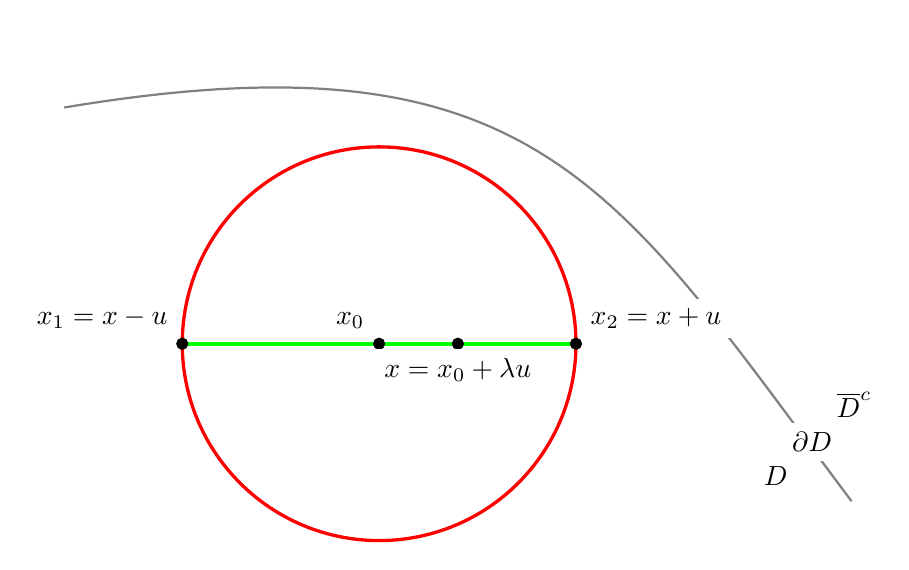
\begin{tikzpicture}
    \draw[gray, thick] (0, 5) .. controls (6, 6) and (7, 4) .. (10, 0);
    \draw[red, very thick] (4, 2) circle(2.5);
    \draw[green, ultra thick] (1.5, 2) -- (6.5, 2);
    \filldraw[black] (4, 2) circle(2pt);
    \node[above left=0pt of {(4, 2)}, outer sep=2pt, fill=white] {\( x_{0} \)};
    \filldraw[black] (5, 2) circle(2pt);
    \node[below =0pt of {(5, 2)}, outer sep=2pt, fill=white] {\(
    x=x_{0}+\lambda u \)};
    \filldraw[black] (1.5, 2) circle(2pt);
    \node[above left=0pt of {(1.5, 2)}, outer sep=2pt, fill=white] {\( x_{1}=x-u \)};
    \filldraw[black] (6.5, 2) circle(2pt);
    \node[above right=0pt of {(6.5, 2)}, outer sep=2pt, fill=white] {\(
    x_{2}=x+u \)};
    \node[above right=5pt of {(9.5, 0.75)}, outer sep=2pt, fill=white] {\( 
    \overline{D}^{c}\)};
    \node[below left=5pt of {(9.5, 0.75)}, outer sep=2pt, fill=white] {\(
    D\)};
    \node[, outer sep=2pt, fill=white] at (9.5, 0.75) {\(
    \partial D\)};
  \end{tikzpicture}

  Let \( u = x - x_{1} \), then \( x_{1} = x - u \), \( x_{2} = x+ u \) and
  there exists some \( \lambda > 0 \) such that \( x = x_{0} + \lambda u \).

  Then, we have
  \begin{align*}
    x = x_{0} + \lambda u = x_{0} + \lambda (x_{2} - x_{0}) = \lambda x_{2} + (1
    - \lambda) x_{0}\\
    \implies f(x) \le \lambda f(x_{2}) + (1- \lambda) f(x_{0})
  .\end{align*}, and
  \begin{align*}
    x &= x_{0} + \lambda u = x_{0} + \lambda ( x_{0} - x_{1}) \\
    &\implies x_{0} = \frac{1}{\lambda + 1} x + \frac{\lambda}{\lambda + 1}
    x_{1}\\
    &\implies f(x_{0}) \le  \frac{1}{\lambda + 1} f(x) + \frac{\lambda}{\lambda +
    1} f(x_{1})
  .\end{align*}

  Let \( M = \sup_{x \in \partial B(x, \varepsilon)} f(x) \) , then \( M \ge
  f(x_{1}), f(x_{2}) \) and \( f(x) \le  \lambda M + (1-\lambda)f(x_{0}) \) and
  \( f(x_{0}) \le \frac{1}{\lambda+1} f(x) + \frac{\lambda}{\lambda+1} M \).
  Another thing to note is that \( M \) is finite due to \( f \) not yielding
  any infinities.

  Hence, we have the following inequalities:

  \begin{align*}
    f(x) - f(x_{0}) &\le  \lambda(M - f(x_{0}))\\
    f(x) + \lambda M &\ge (\lambda + 1) f(x_{0})\\
    \implies f(x) - f(x_{0}) &\ge  \lambda (f(x_{0}) - M)
  .\end{align*}

  Hence, \( 0 \le  |f(x) - f(x_{0})| \le  \lambda (M-f(x_{0})) \), and let \( x \to
  x_{0} \), then \( \lambda \to  0 \) and therefore by the squeeze theorem, \(
  f(x) \to  f(x_{0}) \). Therefore \( f \) is continuous at \( x_{0} \).
\end{proof}

Since we allow infinity values in a convex function \( f \), one would be interested in
the set of points \( x_{0} \) such that \( f(x_{0}) < +\infty \). This set is
called the \textbf{effective domain} of \( f \), denoted as \(
\operatorname{dom} f \). Hence, the above theorem is equivalent to the fact that
\( f \) is continuous on \( \operatorname{Int} \operatorname{dom} f \).

\begin{corollary}[Finite-valued convex functions are closed]
\label{cor:Finite-valued convex functions are closed}
  If \( f: \mathbb{R}^{n} \to  \mathbb{R}  \) is a finite-valued convex function,
  then \( f \) is a closed convex function.
\end{corollary}

\begin{proof}
  Consider a convergent sequence \( (x_{n}, a_{n})_{n \in \mathbb{N}} \) in \(
  \operatorname{epi}  f\) (\( x_{n} \in \mathbb{R}^{n}, a_{n} \in \mathbb{R} \))
  that converges to \( (\overline{x}, \overline{a}) \). We will prove that \(
  (\overline{x}, \overline{a}) \in \operatorname{epi} f \).

  Since \( f \) is continuous, we have:
  \[
    f(\overline{x}) = \lim_{x \to \overline{x}} f(x) = \lim_{n \to \infty}
    f(x_{n}) \le  \lim_{n \to \infty} a_{n} = \overline{a}
  .\] 
  Hence, \( (\overline{x}, \overline{a}) \in \operatorname{epi} f \). Therefore,
  \( \operatorname{epi} f \) contains all of its limit points, which means that
  \( \operatorname{epi} f \) is a closed set.
\end{proof}

% subsection Continuity of convex functions (end)

\subsection{First-order derivative of convex functions} % (fold)
\label{sub:First-order derivative of convex functions}

\begin{theorem}[Partials and convex implies differentiability]
\label{thr:Partials and convex implies differentiability}
  Let \( f: \mathbb{R}^{n} \to \overline{\mathbb{R}}  \) be a convex function
  and \( x_{0} \in \operatorname{Int} \operatorname{dom} f \). Then if \( f \)
  has partial derivatives at \( x_{0} \), then \( f \) is differentiable at \(
  x_{0} \).
\end{theorem}

Note that unlike Theorem \ref{thr:Continuous partials implies
differentiability}, this theorem only requires continuous partial derivatives.

\begin{proof}
  Consider a neighborhood \( B(x_{0}, n\varepsilon) \) and a vector \( d \in B(0,
  \varepsilon) \).

  By the definition of partial derivatives and directional derivatives, we have:
  \begin{align*}
    f(x_{0} + t d) &= f(x_{0}) + \frac{\partial f}{\partial d}(x_{0})t +o(t)\\
    \implies f(x_{0} + t\mathbf{e_{i}}) &= f(x_{0}) + \frac{\partial f}{\partial
    x^{i}}(x_{0}) t + o(t)
  .\end{align*}

  We have:
  \begin{align*}
  f(x_{0} + d) &= f \left( \frac{1}{n}(x_{0} + nd^{i}\mathbf{e_{i}}) \right) \\
  &= \frac{1}{n}f(x_{0} + nd^{i}\mathbf{e_{i}}) \\
  &= \frac{1}{n} \left( f(x_{0}) + n\frac{\partial f}{\partial x^{i}}(x_{0})d^{i} +
  no(d^{i}) \right)  \\
  &= f(x_{0}) + \frac{\partial f}{\partial x^{i}}(x_{0}) d^{i} + o(\|d\|)
  .\end{align*}

  And similarly,
  \[
    f(x_{0} - d) \le  f(x_{0}) - \frac{\partial f}{\partial x^{i}}(x_{0})d^{i} +
    o(\|d\|) \\
  .\] 

  By convexity of \( f \), we have:
  \begin{align*}
    f(x_{0}) &\le \frac{1}{2} \left( f(x_{0} - d) + f(x_{0} + d) \right) \\
    \implies f(x_{0} + d) &\ge 2f(x_{0}) - f(x_{0} - d) \\
                          &\ge 2f(x_{0}) - \left( f(x_{0}) - \frac{\partial f}{\partial x^{i}}(x_{0})d^{i} +
    o(\|d\|) \right) \\
    &= f(x_{0}) + \frac{\partial f}{\partial x^{i}}(x_{0})d^{i} +
    o(\|d\|)\\
    &= f(x_{0}) + f'(x_{0})d + o(\|d\|)
  .\end{align*}

  So, from above, we have \( f(x_{0} + d) \le f(x_{0}) + f'(x_{0})d + o(\|d\|)
  \), and here we have \( f(x_{0} + d) \ge f(x_{0}) + f'(x_{0})d + o(\|d\|) \).
  The two little-o functions don't necessarily have to be the same, so we can
  not naively combine the inequalities to get an equality. However, there is a
  way to get around this, which is the squeeze theorem. Denote the two little-o
  functions as \( h_{1}(d) \) and \( h_{2}(d) \), we have:
  \[
    \frac{h_{1}(d)}{\|d\|} \le \frac{f(x_{0} + d) - f(x_{0}) -
    f'(x_{0})d}{\|d\|} \le \frac{h_{2}(d)}{\|d\|}
  .\] 

  As \( d \to 0 \), the far-left and far-right sides of the inequality tends to
  \( 0 \), and hence the middle expression converges to \( 0 \), which is by
  definition, equivalent to the fact that \( L(h) =
  f'(x_{0})h\) is the multivariable derivative of \( f \) at \( x_{0} \).
\end{proof}

This theorem replaces the requirements of continuous partials by convex, which
is generally harder to prove. In fact, the most conclusive test for convex
function, Theorem \ref{thr:Second derivative convex test}, have the requirement
that \( f \) is differentiable, which is the exact thing we want to prove in the
first place. 

Now, we will be interested in the properties of differentiable convex functions.

First, we have this lemma:

\begin{lemma}
\label{lem:Convex inequality for one variable}
  Let \( f: \mathbb{R} \to \mathbb{R} \) be a single-variable convex function.
  Then, for every \( x < y < z \), we have:
  \[
    \frac{f(y) - f(x)}{y - x} \le \frac{f(z) - f(x)}{z - x} \le \frac{f(z) -
    f(y)}{z - y}
  .\] Moreover, if \( f \) is strictly convex, the above inequalities are strict.
\end{lemma}

\begin{proof}
  The proof of this does not involves any complex (not the \( (a+bi) \)-type of
  complex) multivariable calculus.

  First, we express \( y \) as a linear combination of \( x \) and \( z \):
  \[
    y = \frac{z - y}{z - x}x + \frac{y - x}{z - x}z
  .\] 

  Then, by convexity of \( f \), we have:
  \begin{align*}
    f(y) &\le \frac{z - y}{z - x}f(x) + \frac{y - x}{z - x}f(z)
  .\end{align*}

  Using this, we have:
  \begin{align*}
    f(y) - f(x) &\le (y-x) \frac{f(z) - f(x)}{z - x}  \\
    \frac{f(y) - f(x)}{y - x} &\le \frac{f(z) - f(x)}{z - x}
  ,\end{align*} and:
  \begin{align*}
      f(z) - f(y) &\ge (z - y) \frac{f(z) - f(x)}{z - x}\\
    \frac{f(z)-f(y)}{z - y} &\ge \frac{f(z) - f(x)}{z - x}
  .\end{align*}
\end{proof}

Now, if one let \( y \to x^{+} \), and \( f \) is differentiable at \( x \), \(
\frac{f(y)-f(x)}{y - x} \to f'(x) \). We have the inequality \( \frac{f(z) -
f(x)}{z - x} \ge f'(x) \). Extending this idea to multivariable functions, we
have:
\begin{theorem}
\label{thr:Derivative inequality of convex function}
  Let \( f: \mathbb{R}^{n} \to \mathbb{R} \) be a differentiable
  function. Then, \( f \) is convex if and only if:
  \[
    f(y) \ge f(x) + f'(x)(y-x)
  .\] 
\end{theorem}

\begin{proof}
  If \( f \) is convex, then let \( g(t) = f(x + t(y - x)) \), \( g \) is a
  single-variable differentiable and convex function. Using Lemma
  \ref{lem:Convex inequality for one variable}, we have:
  \[
    g'(0) = \lim_{t \to 0^{+}} \frac{g(t) - g(0)}{t - 0} \le \frac{g(1)-g(0)}{1
    - 0} = f(y) - f(x) 
  .\] 

  Moreover, by Theorem \ref{thr:Multivariable chain rule}, we have \( g'(0) =
  f'(x)(y - x) \), thus \( f'(x)(y - x) \le f(y) - f(x) \).

  To prove the reverse case, consider \( A \subseteq \mathbb{R}^{n}, \lambda \ge
  0\) and denote \(x_{0} = \mathcal{C}(A, \lambda) \). For every \( y \in A \),
  we have \( f(y) \ge f(x_{0}) + f'(x_{0})(y - x_{0}) \), and hence:
  \begin{multline*}
    \mathcal{C}(f(A), \lambda) \ge \mathcal{C}(f(x_{0}) + f'(x_{0})(A - x_{0}),
    \lambda) \ge f(x_{0}) - f'(x_{0})x_{0} + f'(x_{0})\mathcal{C}(A, \lambda)\\ =
    f(x_{0}) - f'(x_{0})x_{0} + f'(x_{0})x_{0} = f(x_{0}) = f(\mathcal{C}(A,
    \lambda)),
  \end{multline*} and \( f \) is a convex function.
\end{proof}

\begin{corollary}[Stationary points of convex programs are GOSes]
\label{cor:Stationary points of convex programs are GOSes}
  If \( f \) is a convex function that is differentiable on \( \mathbb{R}^{n}
  \), then \( x_{0} \) is a GOS of \( (P): \min f(x), x \in \mathbb{R}^{n} \)
  if and only if \( f'(x_{0}) = 0 \).
\end{corollary}

\begin{proof}
  Theorem \ref{thr:Critical point theorem} proved the \( \Rightarrow \) clause,
  so we will only have to prove the reverse direction here.

  Since \( f'(x_{0}) = 0 \), using Theorem \ref{thr:Derivative inequality of
  convex function}, we have \( f(y) \ge f(x_{0}) +f'(x_{0})(y- x) = f(x_{0}) \),
  for all \( y \in \mathbb{R}^{n} \), which means that \( x_{0} \) is a GOS of
  \( (P) \).
\end{proof}


We can make the inequality more "symmetric" by using swapping \( x \) and \( y
\) to get \( f(x) \ge f(y) + f'(y)(x-y)  \). Adding the original inequality to
this yields \( (f'(y)-f'(x))(y - x)\ge 0 \). This inequality is actually
equivalent to the original one (and the fact that \( f \) is convex), but we
will not get into that here.

Going back to affine supports, subgradients and subdifferentials. The value \( c
\) is called the affine support of \( f \) at \( x_{0} \) if \( f(y)-f(x)\ge c(y -
x) \), which fits what we have proven for the \( f'(x) \). Hence, the Jacobian
matrix of a differentiable convex function is an affine support of that function
at that point. And since the transpose of the Jacobian is the gradient, \(
\nabla f(x) \) is a subgradient of \( f \) at \( x_{0} \), which is the
motivation for the naming of subgradient. In fact, if \( f \) is continuously
differentiable (i.e. \( \nabla f \) is continuous) at \( x \), then \( \nabla
f(x) \) is the only subgradient of \( f \) at \( x_{0} \).

% subsection First-order derivative of convex functions (end)

\subsection{Second-order derivative of convex functions} % (fold)
\label{sub:Second-order derivative of convex functions}

Consider the twice-differentiable function \( f: \mathbb{R}^{n} \to \mathbb{R}
\). We would be interested in checking whether \( f \) is convex (or concave or
neither). For single-variable functions, \( f: \mathbb{R} \to \mathbb{R} \) is
convex when \( f''(x) \ge 0 \), and the generalization of this to multivariable
functions is the definiteness of the Hessian matrix:

\begin{theorem}[Second derivative convex test]
\label{thr:Second derivative convex test}
  Let \( f: \mathbb{R}^{n} \to \mathbb{R} \) be a twice-differentiable function.
  Then,
  \begin{itemize}
  \item \( f \) is convex if and only if \( f''(x_{0}) \) is
    positive semi-definite for every \( x_{0} \in \mathbb{R}^{n} \).
  \item If \( f''(x_{0}) \) is positive-definite, then \( f \) is
    strictly convex.
  \end{itemize}
\end{theorem}

\begin{proof}
  The idea is to simply use Theorem \ref{thr:Multivariable Taylor's theorem},
  one can rewrite the Lagrange remainder form to:
  \[
    f(x_{0}+\lambda d)-f(x_{0})-\lambda f'(x_{0})d =\lambda^{2}
    \frac{d^{T}\nabla^{2}f(x_{0} + t d)d}{2}, t \in [0, \lambda],
  \]

  Note that by looking at the sign of the LHS, one can prove that \( f \) is
  convex or strictly convex by Theorem \ref{thr:Derivative inequality of convex
  function}.

  If \( f \) is convex, LHS is positive and therefore so is RHS. Let \( \lambda
  \to 0\), so \( t \to 0 \) and since RHS stays non-negative, we must have \(
  d^{T}f''(x_{0})d \ge 0 \) for all vectors \( d \in \mathbb{R}^{n} \), which
  means \( f''(x_{0}) \) is positive semi-definite.

  If \( f''(x) \) is positive semi-definite for all \( x \in \mathbb{R}^{n} \),
  then the RHS expression is non-negative. Let \( x_{0} + \lambda d = y \), we
  have \( f(y) - f(x_{0}) \ge f'(x_{0})(y - x_{0}) \) holds true for all \( y \)
  and \( x_{0} \). therefore, \( f \) is convex.

  If \( f''(x) \) is positive-definite, then the inequality is strict when \( d
  \neq 0 \), so \( f(y) > f(x_{0}) + f'(x_{0})(y - x_{0}) \) for all \( y \neq
  x_{0}\), which is equivalent to the fact that \( f \) is strictly convex.
\end{proof}

Note that here, \( f \) being strictly convex does not necessarily imply that \(
f''(x_{0})\) is positive-definite. One such counterexample is the function \( f:
\mathbb{R} \to  \mathbb{R}\), \( f(x) = x^{4} \), with \( f''(x) = 12x^2 \),
which is not strictly positive for all \( x \in \mathbb{R} \).

% subsection Second-order derivative of convex functions (end)

\iffalse
\begin{theorem}
  Let \( f \) be a function on open convex set \( D \).

  If \( f \) is convex, then for all directions \( d \neq  0 \),
  \( \frac{\partial f}{\partial d}(x_{0})  \), the
  \textbf{directional derivative} of \( f \) at \( x_{0} \in D \) wrt direction
  \( d \) exists and satisfies \( \frac{\partial f}{\partial d} (x_{0}) \le f(x_{0} + d) -
  f(x_{0}) \) if \( x_{0} + d \in D \).

  If \( f \) is differentiable, \( \nabla f = f'^{T} \) is the \textbf{gradient}
  of \( f \) exists. Then \( f \) is convex iff \( f(y)-f(x) \ge f'(x)(y-x)
   = \langle \nabla f(x), y -x\rangle\) for all \( x,y\in D \). Moreover, \( f
   \) is strictly convex on \( D \) iff equality only holds if \( x = y \).
\end{theorem}

\begin{proof}
  Consider the scalar function \( g(t) = f(x_{0}+t d) \), then \( g \) is
  defined on some neighborhood \( B(0, \varepsilon) \) of \( 0 \).

  We will prove that \( g \) is convex. This is true since \( g(\mathcal{C}(T,
  \lambda)) = f(x_{0} + \mathcal{C}(T, \lambda)d) = f(\mathcal{C}(x_{0} + Td,
  \lambda) \), because of linearity. Since \( f \) is convex \( g(\mathcal{C}(T,
  \lambda)) = f(\mathcal{C}(x_{0}+Td, \lambda)) \le \mathcal{C}(f(x_{0}+Td),
  \lambda) = \mathcal{C}(g(T), \lambda) \), QED.

  Then, we just need to prove that \( g \) has right derivative at \( 0 \). This
  is indeed true, as for any \( 0 < u < v < \varepsilon \), if let \( \lambda =
  \frac{u}{v}\), then \( u = \lambda v + (1 - \lambda) 0 \) and \( g(u) \le
  \lambda g(v) + (1- \lambda)g(0) = \lambda g(v) + (1 - \lambda)g(0) \). Hence,
  \( \frac{g(u) - g(0)}{u} \le  \frac{g(v) - g(0)}{v} \), and the function
  \( h(x) = \frac{g(x) - g(0)}{x} \) is decreasing as \( x \to  0^{+} \). Hence,
  there is a limit \( L = \lim_{x \to 0^{+}} h(x)  \), which is the right
  derivative of \( g(x) \) at \( 0 \). Note that this derivative can be
  (negative) infinity, for example if \( g(x) = -\sqrt[3]{x}  \).

  In the case that \( x_{0} + d \in D \), \( h(1) \) is defined as \( h(1) =
  g(x_{0}  + d) - g(x_{0}) \ge  L = \frac{\partial f}{\partial d}(x_{0})  \), QED.

  Letting \( d = y - x \), then using the identity \( \frac{\partial f}{\partial
  d} (x_{0}) = f'(x_{0})d \) for differentiable \( f \), we have \( f(y)-f(x)
  \ge f'(x)(y-x) \) for all \( x, y \in D \) if \( f \) is convex.

  To prove the reverse direction, let \( x = \mathcal{L}(y, z, w) \) such that \(
  w \in [0, 1]\) (denoting \( \mathcal{L}(x, y, w) = wx + (1-w)y \) as the
  \textbf{linear interpolation} (lerp) from \( x \) to \( y \) with weight \( w \)).
  Then, \( f(z)-f(x) \ge f'(x)(z-x) \) and \( f(y)-f(x) \ge f'(x)(y-x) \).
  Lerping the two inequality: \( \mathcal{L}(f(y)-f(x),f(z)-f(x),w) \ge
  f'(x)\mathcal{L}(y-x, z-x, w) \), yields \( \mathcal{L}(f(y), f(z), w) - f(x)
  \ge  f'(x)(\mathcal{L}(y,z,w)-x\). RHS is \( 0 \) since \( x =
  \mathcal{L}(y,z,w) \), which means \( \mathcal{L}(f(y), f(z), w) \ge
  f(\mathcal{L}(y,z,w) \), which implies that \( f \) is convex.

  To prove the theorem in the strictly convex case, we can trivially use the
  above proof with some obvious modifications.
\end{proof}

Now, consider \( f: D \subseteq \mathbb{R}^{n} \to  \mathbb{R} \), then \(
\nabla f: D \subseteq \mathbb{R}^{n} \to  \mathbb{R}^{n} \), which is a vector
function. Hence, one can define the Jacobian of this function \( (\nabla f)' \).
This matrix, if it exists, is called the \textbf{Hessian} of \( f \). And in
most cases, it's symmetric, hence it could be written as \( (\nabla f)'^{T} =
\nabla ^2 f \). Then, one have the Taylor theorem: for a
twice-continuously-differentiable function \( f \) and \( x_{0}, \Delta x \)
such that \( x_{0}, x_{0} + \Delta x \in \operatorname{dom} f \), then there
exists some \( \theta \in [0, 1] \) such that:

\begin{align*}
  f(x_{0}+\Delta x) &= f(x_{0}) + f'(x_{0})\Delta x + \frac{1}{2} \Delta x^{T}
  \nabla ^2f(x_{0} + \theta \Delta x) \Delta x\\
&= f(x_{0}) + f'(x_{0})\Delta x + \frac{1}{2} \Delta x^{T}
  \nabla ^2f(x_{0}) \Delta x + o(\|\Delta x\|^2)
.\end{align*}

Using this theorem, one can prove the following important result, which can be
used to identify convex functions.

\begin{theorem}[Second derivative test for convex functions]
  Let \( f \) be a twice-continuously-differentiable function on an open convex
  domain \( D \). Then, \( f \) is convex iff \( \nabla ^2 f(x) \) is
  positive semi-definite. Moreover, \( f \) is strictly convex if \( \nabla ^2
  f(x) \) is positive definite.
\end{theorem}

\begin{proof}
  The strictly convex case could be similarly proven.
\end{proof}
\fi

\subsection{Convergence and convergence rate of an algorithm} % (fold)
\label{sub:Convergence and convergence rate of an algorithm}

Every recursive algorithm works by recursively constructing a (potentially
infinite) sequence \( x_{1}, x_{2}, \ldots , x_{n}, \ldots  \). If the algorithm
can find an exact solution, the sequence will only have finitely many steps,
then there exists a map \( T: I \to \mathbb{R} \) that maps every input to the
number of iterations that the algorithm requires. This map can be analyzed to
retrieve the \textbf{time complexity} of the algorithm. Hence, this case is
already solved. For example, the simplex method is \( O(2^{n}) \), which seems
rather inefficient, but it works really well for real-world data.

However, in the case that the sequence \( x_{n} \) is infinite, 

% subsection Convergence and convergence rate of an algorithm (end)

% section Differentiable convex functions (end)

\section{Unimodal optimization algorithms} % (fold)
\label{sec:Single-variable algorithms}

In optimizing mutlivariable functions, sometimes, one would need to solve
univariate nonlinear programs. Here, we will discuss several algorithms to solve
this special class of programs. Additionally, we will only consider a special
class of univariate functions: \textbf{unimodal functions}.

\begin{definition}[Unimodal function]
\label{def:Unimodal function}
  A function \( f: X \subseteq \mathbb{R} \to  \mathbb{R} \) is
  \textbf{unimodal} if there exists \( x_{0} \in X \) such that \( f \) is
  monotonically decreasing on \( X_{-} = \{x \in X, x < x_{0}\}   \) and
  monotonically increasing on \( X_{+} = \{x \in X, x > x_{0}\}   \).
\end{definition}

This definition is not consistent with the traditional one. \( x_{0} \) here is
the global minimum of \( f \) on \( X \), but the original concept of this
function: "functions with one mode (global maximum)". However, the idea is still
the same.

If \( X \) is closed, then \( f \) has a global minimum on \( X \). If
furthermore, \( f \) is a convex function, then one can trivially prove that \(
f\) is unimodal. Much like in binary search, we will use the "structure" of
unimodal functions to find its GOS. For example, if \( X = [a, b] \), pick \(
x_{1}, x_{2} \in [a, b] \), \( x_{1} < x_{2} \). One can determine the segment
which \( x_{0} \) belongs to by simply comparing the values of
\( f(x_{1}) \) and \( f(x_{2}) \). If \( f(x_{1}) > f(x_{2}) \), then \( x_{0}
\in [x_{1}, b] \), and otherwise \( x_{0} \in [a, x_{2}] \). This test allows us
to use the idea of binary search in optimizing unimodal functions.

\subsection{Binary method} % (fold)
\label{sub:Binary method}

The algorithm goes as follows:
\begin{python}
# optimize f on [left, right]
def binary_method(f, left, right):
  epsilon = 1e-3 # or some small constant
  mid = (left + right) / 2
  x1 = mid - epsilon / 2
  x2 = mid + epsilon / 2

  if f(x1) <= f(x2):
    # x0 is in [left, x2]
    if x2 - left <= epsilon:
      # if the range is too small, return x1
      return x1
    else:
      return binary_method(f, left, x2)
  else:
    # x0 is in [x1, right]
    if right - x1 <= epsilon:
      # if the range is too small, return x2
      return x2
    else:
      return binary_method(f, x1, right)
\end{python}

One can trivially see that if \verb|epsilon| is small, then the range
\verb|[left, right]| scales in half each iteration, hence the name
\textit{binary} method.

% subsection Binary method (end)

\subsection{Golden ratio method} % (fold)
\label{sub:Golden ratio method}

The Fibonacci sequence is defined as:
\begin{align*}
  F_{1} &= F_{2} = 1 \\
  F_{n+2} &= F_{n} + F_{n + 1}, n \in \mathbb{N}
.\end{align*}

The explicit formula of \( F_{n} \) is \( F_{n} = \frac{\varphi^{n} -
\phi^{n}}{\varphi - \phi} \), with \( \varphi = \frac{\sqrt{5}  + 1}{2} \) is
the golden ratio, \( \phi =  \frac{1 - \sqrt{5} }{2} \) is \( \varphi \)'s
conjugate. The exact reason why this formula exists is out of the scope, but
using this, we have:
\[
  \lim_{n \to \infty} \frac{F_{n + 1}}{F_{n}} = \varphi
.\] 

The golden ratio is the number \( \varphi = \frac{a}{b} \) that satisfies:
\[
  \frac{a + b}{a} = \frac{b}{a}, \forall a, b > 0, \varphi = \frac{a}{b}.
\]

The idea of this method is to divide the \( [a, b] \) range into subranges, much
like in the binary method, but with a twist. The values of \( x_{1} \) and \(
x_{2} \), the positions that we will evaluate \( f \) at, are shared across
iterations.

In other word, if one divide the \( [a, b] \) range into \( [a, x_{2}] \) and \(
[x_{1}, b]\), using linear interpolation:
\begin{align*}
  x_{1} &= \operatorname{lerp}(a, b, t_{1}) \\
  x_{2} &=  \operatorname{lerp}(a, b, t_{2}) \\
.\end{align*}

Then, in the subranges \( [a, x_{2}] \) and \( [x_{1}, b] \), we have these
division points:
\begin{align*}
  x_{11} &= \operatorname{lerp}(a, x_{2}, t_{1}) \\
  x_{12} &= \operatorname{lerp}(a, x_{2}, t_{2}) \\
  x_{21} &= \operatorname{lerp}(x_{1}, b, t_{1}) \\
  x_{22} &= \operatorname{lerp}(x_{1}, b, t_{2})
.\end{align*}

Now, we have either \( x_{2} = x_{21} \) or \( x_{2} = x_{22} \). We have \(
x_{1} > a \), then \( \operatorname{lerp}(x_{1}, b, t_{2}) >
\operatorname{lerp}(a, b, t_{2}) \), and hence \( x_{22} > x_{2} \). Therefore,
we must have \( x_{2} = x_{21} \), which is equivalent to:
\begin{align*}
  x_{2} &= x_{21} = (1 - t_{1})x_{1} + t_{1}b\\
  &= (1 - t_{1})((1 - t_{1})a + t_{1}b) + t_{1}b \\
  &= (1 - t_{1})^2 a + (2t_{1} - t_{1}^2)b \\
  x_{2} &= (1 - t_{2})a + t_{2}b
,\end{align*}hence \( 1 - t_{2} = (1 - t_{1})^2 \) and \( t_{2} = 2t_{1} -
t_{1}^2 \).

The two equations are actually equivalent (one can add them up to yield \( 1 = 1
\)), so we need to consider the equation for \( x_{1} = x_{12} \):

\begin{align*}
  x_{1} &= x_{12} = (1 - t_{2})a + t_{2}x_{2} \\
  &= (1-t_{2})a + t_{2}((1-t_{2})a + t_{2}b) \\
  &= (1 - t_{2}^2)a + t_{2}^2b \\
  x_{1} &= (1 - t_{1})a + t_{1}b
,\end{align*}hence \( t_{2}^2 = t_{1}\).

Now, we have \( t_{2} = 2t_{2}^2 - t_{2}^{4} \), or equivalently, \( t_{2}(t_{2}
- 1)(t_{2}^2 -t_{2} - 1) = 0 \). Solving this yields \( t_{2} = \varphi \), the
golden ratio. Then, since \( t_{1} = t_{2}^2 = \varphi ^2 \), and \( \varphi ^2
+ \varphi = 1\), we must have \( t_{1} + t_{2} = 1 \), and the division points
\( x_{1} \) and \( x_{2} \) are symmetric wrt the midpoint.

\begin{figure}
  \centering
  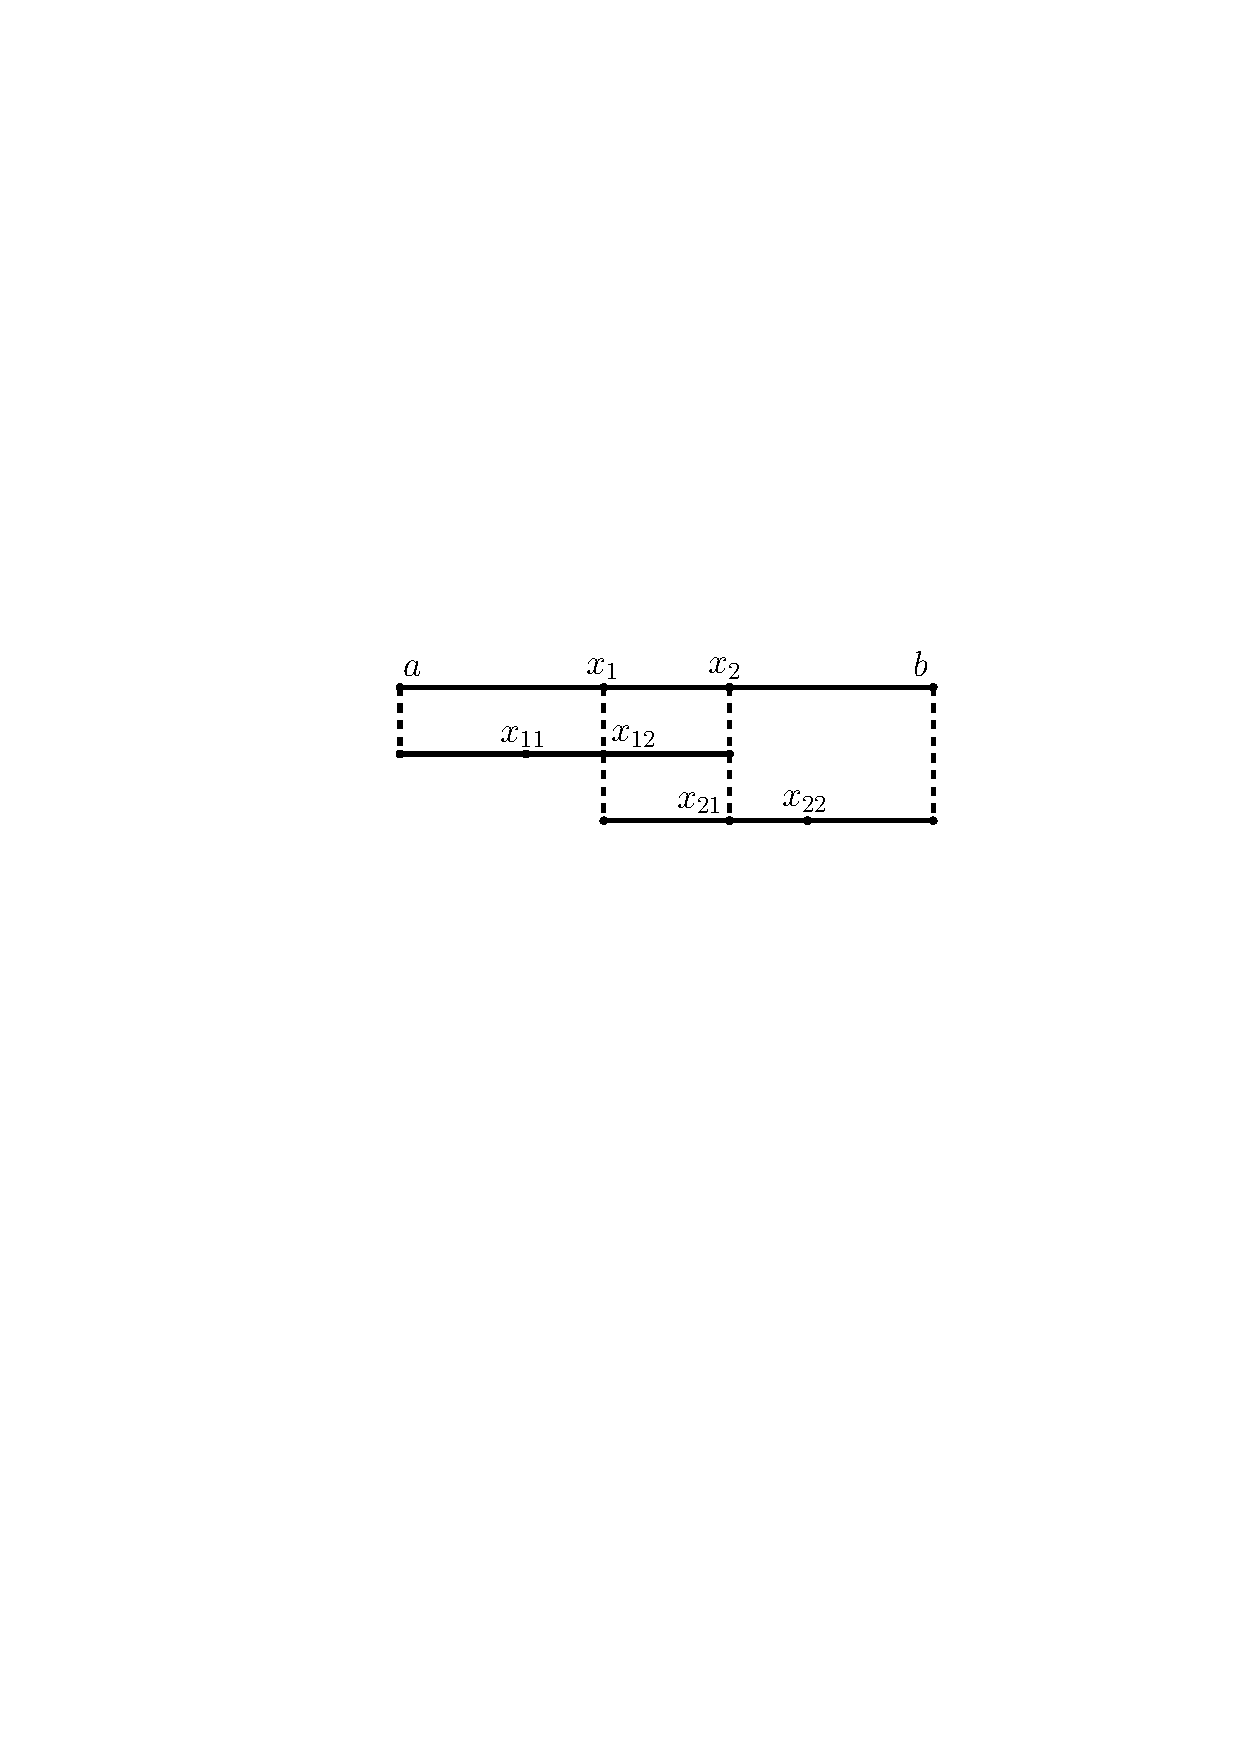
\includegraphics[scale=0.5]{figures/b}
\end{figure}

Using this, we have the golden ratio method (this algorithm will assume that \(
f\) uses memoization, in order to make thing less complicated).
\begin{python}
def golden_ratio_method(f, left, right):
  epsilon = 1e-3 # or some small constant
  golden_ratio = (sqrt(5) - 1) / 2 # > (2 - 1) / 2 = 1/2
  x1 = lerp(right, left, golden_ratio)
  x2 = lerp(left, right, golden_ratio) # since golden_ratio > 1/2, x1 < x2

  if f(x1) <= f(x2):
    # in [left, x2]
    if x2 - left <= epsilon:
      return x1
    else:
      return fibonacci_method(f, left, x2)
  else:
    # in [x1, right]
    if right - x1 <= epsilon:
      return x2
    else:
      return fibonacci_method(f, x1, right)
\end{python}

Aside from the first iteration, the algorithm calculate \( f(x) \) (for a brand
new value of \( x \)) once every
iteration. For complicated objective functions, this can make the algorithm much
faster than the binary method. However, the range scales by \( \varphi^{-1} \)
every iteration, which is slower than the binary method.

Let's do a quick comparison of the two algorithms. Assuming that every
evaluation of \( f \) takes \( F \) units of time, and the control flow of each
iteration takes \( I \) units of time, the number of iterations
needed for the binary method is roughly \( N = \log_{2} L = \frac{\ln L}{\ln  2}
\), with \( L \) being the length of the original range, so the time taken in
the binary method is \( T_{2} = \frac{\ln L}{\ln  2}(2F + I) \). Similarly, the time
taken for the golden ratio method is \( T_{\varphi} = \frac{\ln L}{\ln
\varphi}(F + I) \). The ratio of the two expressions is:
\[
  \frac{T_{2}}{T_{\varphi}} = \frac{(2F + I)\ln \varphi}{(F + I)\ln 2}
.\]

If \( F \ll I \), then this ratio approximately become \( \frac{\ln \varphi}{\ln
2} = 0.69\ldots  \), so the binary method is about \( 31\% \) more efficient
than the golden ratio method. However, if \( F \gg I \), then this ratio become
\( \frac{2 \ln \varphi}{\ln 2} = 1.39\ldots  \), so the golden ratio method is
\( 39\% \) faster. Our premature optimization ends here.

% subsection Golden ratio method (end)

% section Single-variable algorithms (end)

\section{Descent method} % (fold)
\label{sec:Descent method}

The simplex method, introduced in Chapter \ref{chap:Linear programming} is a
variant of the descent method. The idea of this method is very simple: one
simply start from a point \( x_{0} \) in the feasible set (which is
unconstrained in unconstrained linear programs), and look at a local
neighborhood of \( x_{0} \), then move in a direction \( d \) that minimizes \(
f\). If every direction ends up increasing the objective function, by
definition, \( x_{0} \) is a LOS.

If the objective is to find GOSes, one may need to find some method to break out
of the "cages" that LOSes introduces. For example, Genetic Algorithm (GA) uses
mutation to "mutate" its set of potential solutions. This is a very hard
problem, and there are no conclusive solution for this, hence most test
optimization functions (escape for the trivial Sphere function)
are functions that features multiple LOSes and an unique
GOS, in order to test the ability to escape from the cages of LOSes.

Here, we will only be interested in the naive algorithm, not caring about
escaping LOS cages. In other words, we are only interested in finding LOSes.

\subsection{Descent directions} % (fold)
\label{sub:Descent directions}

The descent method requires one to find a direction \( d \) (WLOG assuming \(
\|d\| = 1 \), we are only interested in the direction of this vector, at least
for now) that minimizes \( f \) at some point \( x_{0} \in \mathbb{R}^{n} \).
For example, if \( f \) is differentiable, we have \( \frac{\partial f}{\partial
d}(x_{0}) = f'(x_{0})d = \langle \nabla f(x_{0}), d \rangle \), representing how
\( f \) changes in an infinitesimal neighborhood of \( x_{0} \). To minimize the
inner product in RHS, one simply let \( d = -\frac{\nabla f(x_{0})}{\|\nabla
f(x_{0}\|)} \). Since we are descending using the direction of the gradient,
this method is called \textbf{gradient descent}.

We can generalize this notion to the concept of \textbf{descent direction}.

\begin{definition}[Descent direction]
\label{def:Descent direction}
  Consider the unconstrained nonlinear program \( (P): \min f(x), x \in
  \mathbb{R}^{n} \) and a point \( x_{0} \in \mathbb{R}^{n} \) Then,
  \( d \) is called a \textbf{descent direction} of \( (P) \) at \( x_{0}
    \) if there exists some \( \varepsilon > 0 \) such that \(    f(x_{0} + t d)
    > f(x_{0}) \) for all \( t \in (0, \varepsilon)    \).
\end{definition}

The above result can be formulated into a theorem:

\begin{theorem}[Negative gradient is a descent direction]
\label{thr:Negative gradient is a descent direction}
  If \( f \) is a differentiable function on \( \mathbb{R}^{n} \), then \( d =
  -\nabla f(x_{0}) \) is a descent direction of \( f \) at \( x_{0} \) if \( d
  \neq 0 \). More generally, if \( f'(x_{0})d < 0 \), then \( d \) is a descent
  direction of \( f \).
\end{theorem}

\begin{proof}
  If \( d = -\nabla f(x_{0}) \neq 0 \), then \( f'(x_{0})d = -d^{T}d < 0 \). We
  only need to prove the general statement.

  Since \( \frac{\partial f}{\partial d}(x_{0}) = \langle \nabla f(x_{0}), d
  \rangle < 0 \), by definition of directional derivatives, we have:
  \[
    \lim_{t \to  0^{+}} \frac{f(x_{0} + t d) - f(x_{0})}{t} < 0
  .\] 

  This implies that there exists some \( \varepsilon > 0 \) such that \( \forall
  t \in (0, \varepsilon), f(x_{0} + t d - f(x_{0}) < 0\) and therefore \(
  f(x_{0} + t d) < f(x_{0}) \), \( d \) is a descent direction of \( f \).
\end{proof}

For convex differentiable functions, we have the reverse direction of Theorem
\ref{thr:Negative gradient is a descent direction}.

\begin{theorem}[Descent direction of convex differentiable function]
\label{thr:Descent direction of convex differentiable function}
  Let \( f: \mathbb{R}^{n} \to \mathbb{R}\) be a convex differentiable function.
  Then, \( d \) is a descent direction of \( f \) if and only if \( f'(x_{0})d <
  0\).
\end{theorem}

\begin{proof}
  If \( f'(x_{0})d < 0 \), by the previous theorem, \( d \) is a descent
  direction of \( f \).

  Since \( f \) is convex, by Theorem \ref{thr:Derivative inequality of convex
  function}, we have \( f(x_{0} + \lambda d) \ge f(x_{0}) + \lambda f'(x_{0})d
  \). If \( d \) is a descent direction of \( f \), then there exists some \(
  \lambda > 0 \) such that \( f(x_{0} + \lambda d) < f(x_{0}) \), which means
  that \( f'(x_{0})d < 0 \).
\end{proof}

% subsection Descent directions (end)

\subsection{Exact and inexact line search} % (fold)
\label{sub:Exact and inexact Line search}

Now that we have the direction to iterate towards, we need to specify how much
to translate the original solution.
his factor is called the \textbf{step length}. If the step length is too small, then
the algorithm will need more iterations to converge to a LOS, and if it is too
large, the algorithm will \textit{overshoot}. The 

Now that we have descent directions and step lengths, we can implement the
descent method in pseudocode:
\begin{python}
def descent(f, x0):
  d = find_descent_direction(f, x0)
  if d is not None or some_other_condition():
    return x0
  l = find_step_length(f, x0, d)
  x0 += l * d
  return descent(f, x0)
\end{python}

The most naive way to determine step length is to simply take the step length to
whatever that minimizes \( f \). This method is called \textbf{exact line
search}, since despite it naivety, it's the most efficient (in terms of how many
iterations, not accounting for the time for each iteration) and "exact" way to
solve the problem. The exact step length of a descent direction \( d \) can be
calculated as:
\[
  L(x_{0}, d) \in \operatorname{Argmin}_{t > 0} f(x_{0} + t d)
.\] Here, do note that multiple exact step length can exist concurrently, much
like how there may be many GOSes for an optimization problem.

For example, if one let \( f(x) = \frac{1}{2}x^{T}Ax + bx + c, x \in
\mathbb{R}^{n}, A \in \mathbb{R}^{n\times n}, b \in \mathbb{R}^{1\times n}, c
\in \mathbb{R} \), \( d = -\nabla f(x_{0}) \) and \( A \) is positive-definite,
then one can calculate \( L(x_{0}, d) \) using an explicit formula (without
inverting \( A \)).

First, it is trivial to see that \( f \) is convex, and \( d \) is a descent
direction of \( f \) implies that \( x_{0} \) is not a GOS of \( (P): \min f(x),
x \in \mathbb{R}^{n}\). Then, let \( \varphi(t) = f(x_{0} + t d) \) and use
Theorem \ref{thr:Multivariable chain rule}, we have:
\[
  \varphi'(t) = \frac{df}{d(x_{0} + t d)} \frac{d(x_{0} + t d)}{dt} = f'(x_{0} +
  t d)d
.\]

Substituting \( f'(x) = x^{T}A + b \) to this identity yields:
\[
  \varphi'(t) = ((x_{0}+t d)^{T}A + b)d = (x_{0}^{T}A + b)d + td^{T}Ad
.\] 

Since \( A \) is positive-definite, \( \varphi'(t) \) is an increasing linear
function, which means that \( \varphi \) has a global minimum at \( t_{0} \)
such that \( \varphi'(t_{0}) = 0 \). We can calculate \( t_{0} \) to be:
\[
  t_{0} = -\frac{(x_{0}^{T}A + b)d}{d^{T}Ad}
,\] and this is the exact step length of \( d \).

This expression is very efficient to calculate, since it does not involve any
inefficient operations (the most inefficient one here is probably matrix-vector
multiplication, which is only \( O(n^2) \) complexity).

The descent method that uses exact step length and negative gradient as its
descent direction is called the \textbf{steepest descent} method.

Exact line search only works for simple functions. Here, we will look at how to
roughly estimate a good step length. Since this algorithm is not exact, we will
call such algorithms \textbf{inexact line search}.

These algorithms work by finding the step length \( t_{0} \) such that \(
f(x_{0} + t d) < f(x_{0}) \), and to ensure convergence, \( t_{0} \) must
satisfy several conditions. One such condition is the Armijo conditions. This
works at \( x_{0} \in \mathbb{R}^{n} \)for functions \( f \), but with
additional conditions like \( f \) being Lipschitz continuous and a weird and
complex condition. We will not discuss them here, but for many functions (L.
Armijo described them to be "functions having Lipschitz coninuous first partial
derivatives"), these conditions are satisfied for all \( x_{0} \in
\mathbb{R}^{n} \).

Consider a descent direction \( d \) of \( f \) at \( x_{0} \in \mathbb{R}^{n}
\), we have:
\[
  \frac{\partial f}{\partial d}(x_{0}) = f'(x_{0})d = \lim_{t \to  0^{+}}
  \frac{f(x_{0} + t d) - f(x_{0})}{t} < 0
.\] 

Which is equivalent to:
\[
  \lim_{t \to  0^{+}}  \frac{f(x_{0} + t d) - f(x_{0})}{tf'(x_{0})d} = 1
.\]

Hence, for every \( m \in (0, 1) \), there exists \( t_{0} \) such that \(
\frac{f(x_{0} + t d) -f(x_{0})}{tf'(x_{0})d} \ge  m \), or \( f(x_{0} + t d) \le 
f(x_{0}) + mt f'(x_{0})d \) for all \( t \in (0, t_{0}] \). \textbf{Backtracking
line search} works by finding \( t_{0} \) for some fixed value \( m \). The idea
is simple, one starts with \( t_{0} = t_{max} \) (tipically \( t_{max} = 1 \)), and
decreases \( t_{0} \) by multiplying it with some constant \( \alpha \in (0, 1)
\). To check whether \( t_{0} \) is valid, we will only check the inequality for
\( t = t_{0} \):
\begin{python}
t_max = 1
def backtracking_line_search(f, x0, d):
  jf = jacobian(f, x0)
  t0 = t_max

  while f(x0 + t * d) > f(x0) + m * t0 * jf * d:
    t0 *= alpha

  return t0
\end{python}

% subsection Exact and inexact line search (end)

\subsection{Multivariate Newton's method} % (fold)
\label{sub:Multivariate Newton's method}

Solving for critical points is equivalent to solving \( g(x) = \nabla f(x) = 0 \) (and
find points where \( \nabla f(x) \) is undefined). This is a nonlinear equation,
and there is no general way to solve these. However, there are many
approximation methods for this. One such method is the Newton's method.

The traditional Newton's method is used to find roots of nonlinear
single-variable equations: \( g(x) = 0 \), if \( g \) is a differentiable
function. The idea is simply repeatedly reassigning \( x = x -
\frac{g(x)}{g'(x)} \) until the solution is good enough. Here, we will elaborate
further about the motivation of this formula and more importantly, generalize it
to multivariable functions.

The idea of the method goes as follow. Consider the Taylor expansion at a point
\( x_{0} \in \mathbb{R}^{n} \):
\[
  g(x) \approx g(x_{0}) + g'(x_{0})(x - x_{0})
.\]

If one knows \( g(x_{0}) \) and \( g'(x_{0}) \), and would want to find \( x \)
such that \( g(x) = 0 \), one can approximate \( x \) as:
\begin{align*}
  &0 \approx g(x) = g(x_{0}) + g'(x_{0})(x - x_{0}) \\
  &\implies x - x_{0} \approx - g'(x_{0})^{-1}g(x_{0})\\
  &\implies x \approx x_{0} - g'(x_{0})^{-1}f(x_{0})
.\end{align*}

For some, the generalization from the single-variable formula to this formula is
obvious, since replacing division in \( \mathbb{R} \) by multiplying with
the inverse matrix. We derive it here in order to show the motivation for the
method.

Substituting back \( g = \nabla f \), we have \( g' = \nabla ^2f \) and:
\[
  x = x_{0} - f''(x_{0})^{-1}\nabla f(x_{0})
.\] 

The direction of \( x - x_{0} \), \( -f''(x_{0})^{-1} \nabla f(x_{0}) \) is
called the \textbf{Newton direction} of \( f \) at \( x_{0} \). Here is a
relationship between Newton directions and descent directions:

\begin{theorem}[Newton directions are descent directions]
\label{thr:Newton directions are descent directions}
  If \( f''(x_{0}) \) is positive-definite, then the Newton direction of \( f \)
  at \( x_{0} \): \( n(x_{0}) = -f''(x_{0})^{-1}\nabla f(x_{0}) \) is a descent
  direction of \( f \).
\end{theorem}

\begin{proof}
  One simply calculate \( f'(x_{0})n(x_{0}) \) as follows:
  \begin{align*}
    f'(x_{0})n(x_{0}) = -\nabla f(x_{0})^{T}f''(x_{0})^{-1}\nabla f(x_{0}) < 0
  ,\end{align*} since \( f''(x_{0}) \) is positive-definite (and therefore so is
  its inverse). By Theorem \ref{thr:Negative gradient is a descent direction},
  \( n(x_{0}) \) is a descent direction of \( f \) at \( x_{0} \).
\end{proof}

The Newton's method can utilize constant step length or using backtracking line
search to determine the step length. However, one can see two problems of this method:
\begin{itemize}
\item \( n(x_{0}) \) does not necessarily have to be a descent direction of \( f
  \) at \( x_{0} \).
\item \( f''(x_{0}) \) does not necessarily have to be invertible.
\item Inverting \( f''(x_{0}) \) (or solving for \( n(x_{0}) \) for better
  performance) is very inefficient.
\end{itemize}

To fix this, one can reuse the idea of "caching" like in the simplex method.
However, there are no exact way to calculate \( f''(x)^{-1} \) from \(
f''(x_{0})^{-1} \), so the best thing here is to approximate. This is called the
\textbf{Quasi-Newton methods}. For linear approximations,
this theorem will come in handy:

\begin{theorem}[Sherman-Morrison formula]
\label{thr:Sherman-Morrison formula}
  Let \( A \in \mathbb{R}^{n\times n} \) be an invertible \( n\times n \)
  matrix, then the matrix \( A' = A + uv^{T} \) is invertible if and only if \(
  1 + v^{T}A^{-1}u \neq 0\). In this case:
  \[
    A'^{-1} = A^{-1} - \frac{A^{-1}uv^{T}A^{-1}}{1 + v^{T}A^{-1}u}
  .\] 
\end{theorem}

\begin{proof}
  We have:
  \begin{align*}
    (A + uv^{T})(A^{-1}-\frac{A^{-1}uv^{T}A^{-1}}{1 + v^{T}A^{-1}u}) - I_{n} &= -
    \frac{uv^{T}A^{-1}}{1 + v^{T}A^{-1}u} + uv^{T}A^{-1}
    -\frac{u(v^{T}A^{-1}u)v^{T}A^{-1}}{1 + v^{T}A^{-1}u}\\
    &= uv^{T}A^{-1} -  \frac{u(1 + v^{T}A^{-1}u)v^{T}A^{-1}}{1 + v^{T}A^{-1}u} \\
    &= 0
  .\end{align*}

  To prove the result in the case \( 1 + v^{T}A^{-1}u = 0 \), one can use the
  Matrix determinant lemma. In a nutshell, skipping the details of \( \det(I +
  uv^{T}) = 1 +  u^{T}v = 1 + v^{T}u \), we have:
  \[
    \det A' = \det(A + uv^{T}) = \det(A) \det(I_{n} + A^{-1}uv^{T}) = (1 +
    v^{T}A^{-1}u)\det A
  .\] 

  Hence, one can see that \( A' \) is invertible if and only if \( 1 +
  v^{T}A^{-1}u \neq 0 \), given that \( A \) is already invertible.
\end{proof}

For example, in the Davidon-Fletcher-Powell formula, we update the "approximated
inversed Hessian matrix" using this formula:
\begin{align*}
  u &=  \nabla f(x_{0} + t d) - \nabla f(x_{0}) \\
  v &= H(x_{0})u \\
  H(x_{0} + t d) &= H(x_{0}) + \frac{dd^{T}}{u^{T}d}t - \frac{vv^{T}}{u^{T}H(x_{0})u}
.\end{align*}

As one can see, the formulas here are very complicated, and so is the motivation for
the formula.

% subsection Multivariate Newton's method (end)

% section Descent method (end)

\section{Search algorithms for nondifferentiable functions} % (fold)
\label{sec:Search algorithms for nondifferentiable functions}

Here, we will list two relatively simple search algorithms for nondifferentiable
functions.

\subsection{Hooke-Jeeves method} % (fold)
\label{sub:Hooke-Jeeves method}

\begin{python}
def hooke_jeeves(f, x0):
  delta = 1 # one should start off with a large delta
  epsilon = 1e-3 # a small positive constant
  n = dimensions(x0)
  v = identity(n) * delta

  while True:
    old_x0 = x0
    for i in range(n):
      x0 = argmin(f, [x0, x0 - v_i, x0 + v_i])
    if x0 == old_x0:
      if delta <= epsilon:
        return x0
      else:
        v /= 2
        delta /= 2
    else:
      x0 = 2 * x0 - old_x0
\end{python}

The method basically explores the (discrete) neighborhood of a given point \(
x_{0} \). If \( x_{0} \) is the most optimal, it decreases the step length
(\verb|delta|) and continue searching in a smaller neighborhood, or stop the
algorithm once the precision is sufficient. Otherwise, we move to the point \(
x_{0}' \) that is symmetric to \( x_{0} \) (\verb|old_x0|) across the most
optimal neighbor (\verb|x0|). The matrix \( v \) here simply acts as an array of
standard basis vectors, no matrix operations are done to it (scaling it simply
means scaling all column vectors of \( v \)).

% subsection Hooke-Jeeves method (end)

\subsection{Sequential simplex search algorithm} % (fold)
\label{sub:Sequential simplex search algorithm}

The idea of this algorithm is to construct a simplex, which is the most simple
convex polytope (bounded convex polyhedron) in \( n \) dimensions. Every
iteration, one move or shrink the simplex by looking at the least optimal vertex
of the simplex, and try to replace it with better points. If it can't find any
better points, it simply shrink the simplex at the most optimal simplex. Every
iteration, the algorithm makes the vertices of the simplex "more optimal".

\begin{python}
# calculate the center of gravity of the simplex,
# with weights determined by `f`
def center_of_gravity(vertices, weight_function):
  sum_weights = 0
  center = [0] * dimensions(vertices[0])
  for v in vertices:
    w = weight_function(v)
    sum_weights += w
    center += v * w
  return center / sum_weights

def sequential_simplex(f, simplex_vertices):
  n = dimensions(f)

  if simplex_vertices is None:
    # initialize the simplex on first iteration
    simplex_vertices = []
  
    for _ in range(n):
      vertex = random_vector(n)
      simplex_vertices.append(vertex)

  x_max = argmax(f, simplex_vertices)
  x_min = argmin(f, simplex_vertices)
  i_max = simplex_vertices.find(x_max)
  i_min = simplex_vertices.find(x_min)

  # if the simplex vertices are roughly as optimal, end the program
  if f(x_max) - f(x_min) < epsilon:
    return x_min

  center = center_of_gravity(simplex_vertices, lambda x: abs(f(x)))

  # reflect x_max about center
  x_reflect = 2 * center - x_max

  if f(x_reflect) <= f(x_min):
    # reflect center about x_reflect
    center_reflect = 2 * x_reflect - center

    # replace x_max by a better point
    simplex_vertices[i_max] = center_reflect if f(center_reflect) < f(x_min)
                                             else x_reflect
  elif f(x_reflect) < f(x_max):
    simplex_vertices[i_max] = x_reflect
  else:
    # x_reflect is even worse than x_max
    # so maybe a point between x_max and center is good?
    x_midpoint = (x_max + center) / 2
    if f(x_midpoint) < f(x_max):
      simplex_vertices[i_max] = x_midpoint
    else:
      # we are basically out of points to substitute,
      # so our last resort is to shrink the simplex from x_min
      for i in range(len(simplex_vertices)):
        simplex_vertices[i] = (simplex_vertices[i] + x_min) / 2
  return sequential_simplex(f, simplex_vertices)
\end{python}

% subsection Sequential simplex search algorithm (end)

% section Search algorithms for nondifferentiable functions (end)

\section{Convergence and convergence complexity} % (fold)
\label{sec:Convergence and convergence complexity}

\subsection{Asymptotic notation} % (fold)
\label{sub:Asymptotic notation}

We have been using this notation throughout in this book, so here we will define
them rigorously.

\begin{definition}[Asymptotic notation]
\label{def:Asymptotic notation}
  Consider two functions \( f(x): X_{1} \to  \mathbb{R} \) and \( g(x): X_{2}
  \to \mathbb{R} \) and a point \( x_{0} \) on \( X = \overline{X_{1}} \cap
  \overline{X_{2}}  \). Then, we have:
  \begin{itemize}
  \item If \( \limsup_{x \to x_{0}} \frac{|f(x)|}{g(x)} < +\infty \), or for every
    neighborhood \( B(x_{0}, \varepsilon) \subseteq X \), there exists \( M \)
    such that \( |f(x)| \le Mg(x), \forall x \in B(x_{0}, \varepsilon) \), then
    one can write \( f(x) = O(g(x)) \)
  \item If \( \lim_{x \to x_{0}} \frac{f(x)}{g(x)} = 0 \), or for every \( 
    M > 0\), there exists a neighborhood \( B(x_{0}, \varepsilon) \subseteq X\)
    such that \( |f(x)| \le Mg(x), \forall  x \in B(x_{0}, \varepsilon) \), then
    one can write \( f(x) = o(g(x)) \).
  \item If \( g(x) = O(f(x)) \), one can write this alternatively as \( f(x) =
    \Omega(g(x)) \)\footnote{This is not equivalent to the Big Omega notation of
    Hardy and Littlewood, which is oftenly used in analytic number theory. Here,
    we are using the Knuth definition, which has been extensively used in
    complexity theory}.
  \item If \( g(x) = O(f(x)) \) and \( f(x) = O(g(x)) \), then one can write \(
    f(x) = \Theta(g(x)\).
  \item If \( \lim_{x \to x_{0}} \frac{f(x)}{g(x)} = 1 \), then one can write \(
    f(x) \sim g(x)\)
  \end{itemize}
\end{definition}

This is somewhat an abuse of notation, since we have \( x = O(x) = 2x \), but \(
x\) and \( 2x \) are different functions. Therefore, when asymptotic notation is
used, one can not use the transitive property of equality.

A way to get around this is to use set notation, for example \( f(x) \in O(g(x))
\). Here, \( o(g(x) \), \( O(g(x)) \), \( \Theta(g(x)) \) and \( \Omega(g(x)) \)
can be thought of as set of functions satisfying the respective conditions, and one
can add, multiply these sets with a regular function (or sets of functions)
to get a new set of functions. Since the \( \in \) binary relation is not
transitive, this is very well-defined. But since history is not on our side, we
still have to cope with the original notation.

For example, if there is a some algorithm that process an array with length \( n
\), if one looks at the nitty-gritty details like CPU caches, memory latency and
processing speed, the runtime of the algorithm would be a very complicated
expression. However, one can approximate the runtime as a linear function with
relative to \( n \): \( T(n) = an + b \). Here, calculating the constants \( a \) and
\( b \) would again, be impossible due to all of the details described above. To
solve this, one basically write \( T(n) = O(n) \). This also make things much
easier to handle, for example, if \( T(n) = \sqrt{An^2 + Bn + C}  \), then one
can just reduce the square root sign entirely and write \( T(n) = O(n)  \).
Also, in analyzing algorithmic complexity, one rarely care about the exact
amount of steps. For example, if one have a \verb|int| variable \( i \) loops from
\( 1 \) to \( \lfloor \sqrt{x} \rfloor \), we can skip the flooring in
complexity analysis, resulting in something like a \( O(\sqrt{n} ) \)
algorithm.

An asymptotic identity, by its definition, can be thought of a limit, and
therefore, must be handled carefully. One can add and multiply both sides, much
like limits, but just like limit, one can't use the transitive property of
equality, for example.

Going back to the definition, we have the set \( \overline{X}  \), which is the
closure of \( X \). This is to extend the set of feasible \( x_{0} \)'s to a
wider range. For example, most functions works only with the real numbers, and
not \( +\infty \), but in the \( \overline{\mathbb{R}} = \mathbb{R} \cup \{\pm
\infty\}    \) topology, the closure of \( \mathbb{R} \) is \(
\overline{\mathbb{R}}  \), and hence, one can use this notation for \( x_{0} =
+\infty \). This is used extensively in complexity analysis, since the input of
algorithms were generally considered to be very large. The variable \( x_{0} \)
is oftenly induced from the situation. If one is looking at the complexity of
algorithms, \( x_{0} = +\infty \). But in things like the Taylor series, \(
x_{0} = 0 \).

\iffalse
Here is a little fun theorem that relates this and convex analysis.

\begin{theorem}[Big-O functions form a convex cone]
\label{thr:Big-O functions form a convex cone}
  Let \( O(f(x)) \) be the set of functions \( g(x) \) such that \( g(x) =
  O(f(x)) \) (as \( x \to x_{0} \) for some fixed \( x_{0} \)).
  Then, \( O(f(x) \) is a convex cone in the linear space of
  functions (with the same domain and codomain as \( f \)).
\end{theorem}

\begin{proof}
  Let \( A\subseteq O(f(x)) \). Then for every \( a(x) \in A \), we have:
  \[
    \limsup_{x \to x_{0}} \frac{|a(x)|}{f(x)} < +\infty
  .\] 

  Then, for we have:
  \begin{align*}
    \limsup_{x \to x_{0}} \frac{|\mathfrak{C}(A, \lambda)(x)|}{f(x)} 
    &\le
    \left| \limsup_{x \to x_{0}} \frac{\mathfrak{C}(A, \lambda)(x)}{f(x)}
    \right| \\
    &= \left|\mathfrak{C}\left(\limsup_{x \to x_{0}}\frac{A(x)}{f(x)}, \lambda
    \right)\right|\\
    & \le \mathfrak{C} \left( \limsup_{x \to x_{0}} \frac{|A(x)|}{f(x)}, \lambda
    \right) \\
    &< \mathfrak{C}(\{+\infty, +\infty, \ldots \}, \lambda )\\
    &< +\infty
  .\end{align*}

  Hence, \( \mathfrak{C}(A, \lambda) \in O(f(x)) \)
\end{proof}
\fi

% subsection Asymptotic notation (end)

\subsection{Convergence rate of sequences} % (fold)
\label{sub:Convergence rate of sequences}

All of the above algorithms work recursively, and they basically start from a
point \( x_{0} \), find a more optimal point \( x_{1} \), find a even more
optimal point \( x_{2} \), etc. until the stop condition has been reached.
Hence, these algorithms basically produces sequence of solutions for each
optimization problem. Assuming that we give the algorithm no stopping condition
(i.e. we want infinite precision), and even when an optimal solution has been
reached, the algorithm would repeat that solution in this sequence, every
invocation of an optimization algorithm produces an infinite list. We can now
judge how good the algorithm is (num-of-iteration-wise), by looking at the
\textbf{convergence rate} of this sequence.

\begin{definition}[Convergence rate of a sequence]
\label{def:Convergence rate of a sequence}
  Let \( (x_{n})_{n \in \mathbb{N}} \) be a convergent sequence: \( x_{n}\to
  x^{*} \) as \( n \to +\infty \).

  We say that \( x_{n} \) converges with order \( q \) and with factor \( \gamma  \)
  if:
  \[
    \gamma \ge  \limsup_{n \to +\infty} \frac{\|x_{n + 1} -
    x^{*}\|}{\|x_{n} - x^{*}\|^{q}}
  .\] 

  This is equivalent to:
  \[
    0 \le \|x_{n + 1} - x^{*}\| \le \gamma \|x_{n} - x^{*}\|^{q}, \text{for
    arbitrary large } n \in \mathbb{N}
  .\] 
\end{definition}

We have some special cases:
\begin{itemize}
\item If \( q = 1 \), \( \gamma = 1 \), we say convergence is sublinear.
\item If \( q = 1 \), \( \gamma \in (0, 1) \), we say convergence is linear.
\item If \( q = 1 \), \( \gamma = 0 \), we say convergence is superlinear.
\item If \( q = 2 \), we say convergence is quadratic.
\item If \( q = 3 \), we say convergence is cubic.
\end{itemize}

Quadratically convergent and cubically convergent sequences also converges
superlinearly.

When an iterative method solves an optimization problem, it generates many
sequences: \( x_{n} \), the argument sequence, \( f(x_{n}) \), the objective
value sequence, and for problems with differentiable objective functions, there
is also the gradient sequence \( \nabla f(x_{n}) \). Some sequences are derived
from the sequence \( f(x_{n}) \). First, the error sequence \( e_{n} = f(x_{n})
- f^{*}\) (\( f^{*} = \lim_{n \to \infty} f(x_{n}) \) and the error digit count
sequence \( d_{n} = -\log e_{n} \).

Here, the error sequence represents how unoptimal the current solution is, and
the error digit count sequence shows how many accurate digits the current error
is.

We look at some examples:

\textbf{Example} Consider the simple geometric proession:
\[
  x_{0} = 1, x_{1} = \frac{1}{2}, x_{2} = \frac{1}{4}, \ldots , x_{n} =
  2^{-n},\ldots 
.\] 

This sequence converges linearly, with \( q = 1, \mu  = \frac{1}{2} \). We have
\( N(\varepsilon) = -\log _{2} \varepsilon = O(-\log \varepsilon) = O(\delta) \).

\textbf{Example} Consider a faster converging sequence:
\[
  x_{0} = \frac{1}{2}, x_{1} = \frac{1}{4}, x_{2} = \frac{1}{16}, x_{3} =
  \frac{1}{256}, \ldots ,x_{n} = 2^{-2^{n}}, \ldots 
.\] 

This sequence converges quadratically, with \( q = 2, \mu  = 1 \). We have \(
N(\varepsilon) = \log_{2} (-\log _{2} \varepsilon) = O(\log O(\delta)) \).

\textbf{Example} Consider the algorithm that calculate \( \pi  \), in every
iteration of it, it yields a new digit of in the decimal expansion of \( \pi
\), i.e.
\[
  x_{0} = 3, x_{1} = 3.1, x_{2} = 3.14, x_{3} = 3.141, x_{4} = 3.1415,\ldots 
.\] 

Then, we have \( 0 < |x_{n} - \pi| < 10^{-n} \) for all \( n \in \mathbb{N} \).
Using this, we can have an estimate for \( N(\varepsilon) \) as \(
N(\varepsilon) = O(-\log \varepsilon) = O(\delta) \).

This sequence has \( q = 1 \) and \( \mu = \frac{1}{10} \). This combination of
order of convergence and rate of convergence is \textbf{linear rate}. More
generally, a sequence converges with linear rate if it has order of convergence
\( q = 1 \) and rate of convergence \( \mu \in (0, 1) \). When \( \mu = 0 \) and
\( \mu = 1 \), it is called \textbf{sublinear rate} and \textbf{superlinear
rate}, respectively.

\textbf{Example} Consider the algorithm that calculate \( \ln 2 \) by the series:
\[
  \ln 2 = \sum_{n = 1}^{+\infty} \frac{(-1)^{n+1}}{n} =
  1-\frac{1}{2}+\frac{1}{3}-\frac{1}{4}+\ldots 
.\] 
(Here, \( x_{n} \) is the \( n \)-th partial sum of this series \( x_{n} = \sum_{k =
1}^{n} \frac{(-1)^{k + 1}}{k} \).)

The error terms are:
\[
  e_{n} = \sum_{k = n + 1}^{+\infty} \frac{(-1)^{n+1}}{n + 1} = O \left(
  \frac{1}{n} \right) 
.\]
(This result is unproven, since it's outside the scope of what we are discussing
here.)

In optimization problems, if a method achieves convergence, then there are many
\textit{convergent things}: \( x_{n} \to x^{*} \), \( f(x_{n}) \to x^{*} \) or \(
f'(x_{n}) \to 0 \) (for differentiable problems). The convergence theorems
basically prove that one of the \textit{things} mentioned above is convergent, but it
does not necessarily mean that the \textit{other things} are convergent too, and
obviously, knowing the convergent rate of one \textit{thing} does not
necessarily implies that of the other \textit{things}.

Here, we will mostly look at the convergence of the sequence \( f(x_{n}) \), and not
\( x_{n} \). This is somewhat easy to see why, since the quantities like gradients, the
Hessian, etc. talk about the change in \( f \) (with relative to the change in
\( x \), but the main thing is still about the change in \( f \)). Assuming an
algorithm generates
the sequence \( x_{0}, x_{1}, \ldots  \) that converges to \( x^{*} \) (or
weaker, \( f(x_{k}) \) converges to some value \( f^{*} \), which will be
denoted as \( f(x^{*}) \) here),
we denote the \( k \)-th \textbf{error} as \( e_{k} = f(x_{k}) - f(x^{*}) \).
Note that this term is always non-negative, since \( x_{n} \) is a
non-increasing sequence.
We also don't really talk much about the error, but rather how many digits of
them are certain. This amount is represented by the sequence \( d_{n}= -\log
e_{n} = \log \frac{1}{e_{n}}  \).

For some value of \( \varepsilon > 0 \), denote \( N(\varepsilon) \) as the
minimum value of \( N \) such that \( e_{n} < \varepsilon, \forall  n \ge N \).
Then, one can use asymptotic notation to write \( N(\varepsilon) \). Here, one
implicitly let \( \varepsilon \to 0 \). We also denote \( \delta = -\log
\varepsilon \), representing the number of digits in \( \varepsilon \).


Hence, one can see that \( N(\varepsilon) = O \left( 1 / \varepsilon
\right)  = O(10^{\delta}) \). This is called \textbf{exponential time}. And as
one can see, for every new digit of \( \ln 2 \), the algorithm takes more and more
iterations to compute. This is very inefficient.

This sequence has \( q = 1 \) and \( \mu = 1 \). As discussed above, this
sequence converges sublinearly.

We will generalize this result further.

\begin{theorem}[Iteration complexity of linear convergence]
\label{thr:Iteration complexity of linear convergence}
Let \( x_{n} \) be a convergent sequence with rate of convergence \( \mu \in[0,
1]  \) and order of convergence \( q = 1 \). Then, denote \( \delta = -\log
\varepsilon \), we have:
\begin{itemize}
\item If \( \mu  = 0 \), then \( N(\varepsilon) \le O(\log \delta) \).
\item If \( \mu = 1 \), then \( N(\varepsilon) \le  O(1 / \varepsilon) \).
\item Otherwise, \( N(\varepsilon) \le  O(\delta) \).
\end{itemize}
\end{theorem}

\begin{proof}
  We have:
  \[
    \lim_{n \to +\infty} \frac{\|x_{n + 1} - x^{*}\|}{}
  .\] 
\begin{itemize}
\item If \( \mu  = 1 \), then we have:
\item If \( \mu  = 0 \), then we have:
  \[
    1 = \lim_{n \to \infty} \frac{e_{n + 1} - e_{n}}{e_{n}} 
  .\] 
  using the definition of limits, for every \(
  \varepsilon_{0} > 0 \), there exists some \( M(\varepsilon_{0}) > 0 \)
  such that:
  \[
    0 \le  e_{n + 1}  \le \varepsilon_{0} e_{n}, \forall n \ge  M(\varepsilon_{0}) 
  .\] 

  Repeatedly using this, we have: \( e_{n + N} \le \varepsilon_{0}^{n} e_{N}, \forall N \ge
  M(\varepsilon_{0}), n \in \mathbb{N}\). Then, if \( \varepsilon_{0} ^{n}e_{N} <
  \varepsilon \), then \( e_{n + N} < \varepsilon \), which is equivalent to \(n
  > \frac{\log \varepsilon_{0} - \log e_{N}}{\log e_{N}}
  \)

\end{itemize}
\end{proof}

We can look at how fast \( e_{k} \) converges. By the above definition, we have
\( e_{n + 1} \approx \mu e_{n}^{q} \). Repeatedly using this approximation, we
have:
\begin{align*}
  e_{n + N} &\approx \mu e_{n + N - 1}^{q} \\
            &\approx \mu^{1 + q} e_{n + N - 2}^{q^2}\\
            &\approx \ldots \\
            &\approx \mu ^{1 + q + \ldots  + q^{n}}e_{N}^{q^{n}}
.\end{align*}

Here, \( N \) is a very large number, and because of that, \( e_{N} \) would be
very small. Here, we will let \( e_{N} \in (0, 1) \) to get a juicy
"geometric-like progression". 
\iffalse
The \( \mu^{1 + q + \ldots +q^{N}}  \) term here
is basically insignificant\footnote{A more careful analysis works as follows. If
\( q \le  1 \), then since \( x_{n} \) converges, \( \mu \in [0, 1] \), then this
term even make the error smaller. Otherwise, \( q > 1 \) makes \( q^{2^{n}} \) a
geometric progression that grows super fast. That and the fact that it is the
exponent of a power with base \( e_{N} \in (0, 1) \) make the \( \mu^{1 + q +
\ldots  + q^{n}} \) basically a nothing-burger.}
, so we will omit that term.
\fi
Taking the logarithm of both sides yields:
\[
  d_{n + N} \approx -\log e_{n + N} \approx -(1 + q + \ldots  + q^{n})\log \mu +
  q^{n}d_{N}
.\]
If \( q < 1 \), the convergence is painfully slow. If we have developed some
algorithm that have that convergence rate, we may as well throw that algorithm
into the trash can.

If \( q > 1 \), then we can have this estimation:
\[
  d_{n + N} \approx q^{n} \left( d_{N} + \frac{\log \mu}{q - 1} \right)
.\] 

When \( N \) is large, \( d_{N} \gg -\frac{\log \mu}{q - 1} \), and therefore \(
d_{n + N} \approx q^{n}d_{N}\), \( d_{n} \) can be thought of as a geometric
series, so it grows very quickly. In other words, the more iterations we run,
the more digits each iteration would give us.


If \( q = 1 \), we have three cases:
\begin{itemize}
\item \( \mu = 0 \): \textbf{superlinear rate}. Here, 
\end{itemize}

For linearly convergent sequences, we have \( q = 1 \), and since \( x_{n} \)
converges, we must have the rate of convergence \( \mu \in [0, 1] \). \( \mu = 0
\) is superlinear rate, \( \mu = 1 \) is sublinear rate, and \( \mu  \in (0, 1)
\) is simply linear rate.

Now, we will look at how \textit{good} superlinear rate is. Unwrapping the
limit, for every \( \varepsilon > 0 \), there exists some \( N > 0 \) such that:
\[
  (\mu - \varepsilon)\|x_{n}-x^{*}\| \le 
  \|x_{n+1}-x^{*}\| \le 
  (\mu + \varepsilon)\|x_{n}-x^{*}\|, \forall n \ge  N
.\]

Applying this multiple times yields:
\[
  0 \le \|x_{n + N} - x^{*}\| \le (\mu + \varepsilon)^{n}\|x_{N} - x^{*}\|
.\] 

Pick \( \varepsilon \) such that \( \mu + \varepsilon \in (0, 1) \), one ends up
with roughly this rate of convergence: \( \|x_{n} - x^{*}\| \sim
\mu^{n} \). Then, if one wants the estimation error to be at most \( \varepsilon
\), one just need \( O \left( \log  \right)  \)

% subsection Convergence rate of sequences (end)

\subsection{Convergence theorems} % (fold)
\label{sub:Convergence theorems}

In this section, we will discuss results about convergence of the algorithms
that we introduced earlier in this section. First, we have the notion of
\textbf{Lipschitz continuity}.

\begin{definition}[Lipschitz continuity]
\label{def:Lipschitz continuity}
  Let \( (X, d_{X}) \) and \( (Y, d_{Y}) \) be metric spaces and \( f: X \to Y
  \). Then, we say that \( f \) is Lipschitz continuous on \( X' \subseteq X
  \) with constant \( M > 0 \) if:
  \[
    d_{Y}(f(x_{1}), f(x_{2})) \le Md_{X}(x_{1}, x_{2}), \forall  x_{1}, x_{2}
    \in X'
  .\] 
\end{definition}

One can proves that Lipschitz continuity implies continuity pretty easily. To
prove \( f \) is continuous at \( x_{0} \in X \), we need to prove that for
every \( \varepsilon > 0 \), there exists some \( \delta \) such that \(
d_{Y}(f(x), f(x_{0})) < \varepsilon \) for all \( x \in B(x_{0}, \delta) \).
This can be achieved by letting \( \delta = \frac{\varepsilon}{M} \).

Now we will look at the convergence of descent method. First, we will look at
convergence of the classic gradient descent method (with fixed step length).

\begin{theorem}[Convergence of gradient descent with fixed step length]
\label{thr:Convergence of gradient descent with fixed step length}
  Let \( f: \mathbb{R}^{n} \to \mathbb{R} \) be a convex and differentiable
  function, and its gradient is Lipschitz continuous with constant \( M > 0
  \). If \( t \in\left( 0, \frac{1}{L} \right]  \) is the step length of a
  gradient descent process, which yields the value \( x_{k} \) after \( k \)
  iterations, then:
  \[
    f(x_{k}) - f(x^{*}) \le \frac{1}{2tk}\|x_{0}-x^{*}\|^2
  ,\] with \( x^{*} \) denoting the global minimum of \( f \).
\end{theorem}

Using this inequality, we can trivially see that \( f(x_{k}) \to f(x^{*}) \) as
\( k \to +\infty \). This means that \( x_{k} \) will converge to a point as
optimal as \( x^{*} \). Note that \( f \) here is convex, and in a convex
optimization problem, all LOSes are GOSes. So we don't need to worry about
whether \( x_{k} \) converges to a LOS or not.

\begin{proof}
  From the definition of the multivariable derivative, applied to \( f''(x) \):
  \[
    \lim_{h \to 0} \frac{|\nabla f(x_{0}+h)-\nabla f(x_{0}) - f''(x_{0})h|}{\|h\|} = 0
  .\] 

  Substitute \( h = tv \) for some fixed \( v \in \mathbb{R}^{n} \), we have:
  \[
    \|f''(x_{0})v\| = \lim_{t \to 0^{+}} \frac{|\nabla f(x_{0}+tv)-f(x_{0})|}{t} \le
    \lim_{t \to  0^{+}} \frac{L\|x_{0} + tv - x_{0}\|}{t} = L\|v\|
  .\] 

  Using this, we have \( |v^{T}f''(x_{0})v| \le \|v\| \|f''(x_{0})v\| \le
  L\|v\|^2\). Now using the Lagrange remainder form of Theorem
  \ref{thr:Multivariable Taylor's theorem}, for some \( \theta \in [0, 1] \), we have:
  \begin{align*}
    f(x_{0} + h) &= f(x_{0}) -f'(x_{0})h +\frac{1}{2} h^{T}f''(x_{0} + \theta h)h\\
                 &= f(x_{0})-f'(x_{0})h+\frac{1}{2} L\|h\|^2
  .\end{align*}

  Substitute \( x_{0} = x_{k} \) and \( h = x_{k+1} - x_{k} = -t\nabla f(x_{k})
  \), we have:
  \begin{align*}
    f(x_{k+1}) &= f(x_{k}) - t\|\nabla f(x_{k})\|^2 + \frac{1}{2}Lt^2\|\nabla
    f(x_{k})\|^2  \\
    &= f(x_{k}) - t\|\nabla f(x_{k})\|^2 \left( 1 - \frac{Lt}{2} \right)  \\
    &\le f(x_{k}) - \frac{1}{2}t \|\nabla f(x_{k})\|^2
  .\end{align*}

  This is a really interesting result. It showed that, if we knew the value for
  \( L \), then we can always pick a step length that always decrease the
  objective function in every step of gradient descent. Note that this does not
  rely on the condition \( f \) is convex, so this inequality also holds for
  nonconvex functions with Lipschitz continuous gradient.

  Now, using Theorem \ref{thr:Derivative inequality of convex function}, we
  have:
  \begin{align*}
    &f(x^{*}) - f(x_{k}) \ge f'(x_{k})(x^{*} - x_{k})\\
    \implies &f(x_{k})\le f(x^{*})+f'(x_{k})(x_{k}-x^{*})
  .\end{align*}

  Substitute this to the above inequality, we have:
  \begin{align*}
    f(x_{k+1}) - f(x^{*}) &\le f'(x_{k})(x_{k}-x^{*}) - \frac{1}{2t}\|\nabla
    f(x_{k})\|^2\\
    &= \frac{1}{2t} \left( 2t \nabla f(x_{k})^{T}(x_{k}-x^{*}) - \|\nabla
    f(x_{k})\|^2 - \|x_{k} - x^{*}\|^2 \right)  + \frac{1}{2t}\|x_{k}-x^{*}\|^2\\
    &= -\frac{1}{2t}\|x_{k} - t\nabla f(x_{k}) - x^{*}\|^2 +
    \frac{1}{2t}\|x_{k}-x^{*}\|^2\\
    &= \frac{1}{2t}\left( \|x_{k}-x^{*}\|^2 - \|x_{k+1}-x^{*}\|^2 \right) 
  .\end{align*}

  Taking the sum as \( k \in 0..(n - 1) \) yields:
  \begin{align*}
    \sum_{k=0}^{n-1} \left( f(x_{k+1}) - f(x^{*}) \right) &\le \frac{1}{2t}
    \left( \|x_{0}-x^{*}\|^2 - \|x_{n}-x^{*}\|^2 \right) \le
    \frac{\|x_{0}-x^{*}\|^2}{2t}
  .\end{align*}

  Now, note that the terms of the LHS sum are non-increasing, we have the following
  inequality:
  \[
    f(x_{n}) - f(x^{*}) \le \frac{1}{2nt}\|x_{0}-x^{*}\|^2
  .\] 
\end{proof}

Moving to the steepest descent algorithm. It seems to be more "efficient" than
the naive gradient descent, so one would expect it to converge similarly, and
maybe with less conditions (especially convexity). The following theorem proves
that, but the suprising thing is not only does one not need convexity, but
without the Lipschitz continuity condition, the algorithm would still converge!

\begin{theorem}[Global Convergence of Steepest Descent]
\label{thr:Global Convergence of Steepest Descent}
  Let \( f: \mathbb{R}^{n} \to \mathbb{R} \) be a continuous differentiable
  function. Start the steepest descent progress with initial point \( x_{0} \)
  such that the lower level set \( L = L_{f(x_{0})}^{-}(f) \) is bounded (and
  therefore compact), then the algorithm will converges to a stationary point \(
  x^{*} \) of \( f \), i.e. \( f'(x^{*}) = 0 \).
\end{theorem}

\begin{proof}
  Denote the value yielded at iteration \( k \) of the algorithm as \( x_{k} \).
  One can trivially see that \( f(x_{k}) \) is a non-increasing
  sequence. Since \( L \) is closed, \( m = \min_{x \in \mathbb{R}^{n}} f(x) =
  \min_{x \in L} f(x) \) exists, and therefore \( f(x_{k}) \) is bounded below.
  This means that \( f(x_{k}) \) converges as \( k \to
  +\infty \).

  Now assuming that \( \|\nabla f(x_{k})\| \) does not converge to \( 0 \), i.e.
  there exists some \( \varepsilon > 0 \) such that \( \|\nabla f(x_{k})\| \ge
  \varepsilon \) for infinitely many \( k \in \mathbb{N} \). Denote \( i_{k} \)
  as the \( k \)-th index of \( i \) satisfying this inequality, then \(
  x_{i_{k}} \) is a infinite sequence and \( x_{i_{k}} \in L \). Since \( L \)
  is closed, by the \textit{Bolzano-Weierstrass Theorem}, there exists a
  subsequence \( x_{j_{k}} \) of \( x_{i_{k}} \) that converges to \( z \).
  Trivially, we have \( \|\nabla f(z)\| > 0 \).

  By Theorem \ref{thr:Multivariable Taylor's theorem}, we have:
  \[
    f(z - t \nabla f(z)) = f(z) - t\|\nabla f(z)\|^2 + o(t) \le f(z) -
    \frac{1}{2}t \|\nabla f(z)\|^2
  .\] 

  The last inequality holds for arbitrary small \( t \), since \( o(t) \le
  \frac{1}{2}t \|\nabla f(z)\|^2 \) holds for such values of \( t \). Pick \(
  t_{0} \) as one such value of \( t \), then we have:
  \begin{align*}
    f(x_{j_{k} + 1}) &= \min_{t \ge 0} f(x_{j_{k}} - tf'(x_{j_{k}}))\\
    &\le f(x_{j_{k}}-t_{0}\nabla f(x_{j_{k}})) \\
    &= f(x_{j_{k}}-t_{0}\nabla f(x_{j_{k}})) - f(z - t_{0}\nabla f(z)) + f(z -
    t_{0}\nabla f(z)) \\
    &\le  f(x_{j_{k}}-t_{0}\nabla f(x_{j_{k}})) - f(z - t_{0}\nabla f(z)) + f(z) -
    \frac{t_{0}}{2}\varepsilon ^2 \\
  .\end{align*}

  Subtracting \( f(x_{j_{k}}) \) from both sides and let \( k \to +\infty \):
  \[
    \underbrace{f(x_{j_{k}}+1) - f(x_{j_{k}})}_{\to 0}
     \le 
     \underbrace{\left( 
    f(x_{j_{k}}-t_{0}\nabla f(x_{j_{k}})) - f(z - t_{0}\nabla f(z))
\right)}_{\to 0}
+ \underbrace{(f(z) - f(x_{j_{k}}))}_{\to 0} -
    \frac{t_{0}}{2}\varepsilon ^2 \\
  .\] 

  Here, the last two convergence is due to \( f \) being continuous and \(
  x_{j_{k}} \) converges to \( z \). The first one is the result of the fact
  that \( f(x_{k}) \) converges, proved right at the start of the proof.
  Hence, we must have \( t_{0}\varepsilon ^2 \le 0 \), which contradicts with \(
  t_{0} > 0\) and \( \varepsilon \neq 0 \).
\end{proof}

Despite this nice result, the real world still found an optimization problem to
mess with this method. This is due to the hardware limitation of computers,
unable to represent infinite precision and therefore prone to numerical errors.
This nonlinear program is to minimize the Rosenbrock function, which is a very
simple function: \( f(x, y) = 10(y-x^2)^2+(x-1)^2 \).

For inexact line search methods, if can ensure that the step length of each
iterations satisfies certain conditions, then one can prove the convergence of
the algorithm will converge to a stationary point. Such conditions had been
used above in the Backtracking line search algorithm. One may think as condition
as \textit{constraints} that we must satisfy to make thing work, but in reality,
they act more like \textit{clues}, helping us find better and better step
lengths for our algorithm. Remember, if the conditions listed in these theorems
could not be ensured, it does not mean that our algorithm is going to fail,
we just simply lose the certainty for it to work. And as one can see above, even
when the conditions are met, factors like float precision can always cause
issues.

Without further ado, here is \textbf{Zoutendijk's Theorem}, a valuable result in
proving the convergence of inexact line search methods.

\begin{theorem}[Zoutendijk's Theorem]
\label{thr:Zoutendijk's Theorem}
  Let \( f: \mathbb{R}^{n} \to \mathbb{R} \) be a continuous
  differentiable function, \( f \) is bounded below and its gradient is
  Lipschitz continuous on \( \mathbb{R}^{n} \).

  In the descent method, let the descent direction of the \( k \)-th iteration
  be \( d_{k} \), and the step length \( \alpha_{k} \) satisfies the Wolfe
  condition, which is:
  \begin{itemize}
  \item Armijo's condition: \( f(x_{k+1}) \le f(x_{k}) +
    m\alpha_{k}f'(x_{k})d_{k} \), for some \( m > 0 \)
  \item Curvature condition: \( f'(x_{k + 1})d_{k} \ge
    m'f'(x_{k})d_{k} \), for some \( m' < 1 \).
  \end{itemize}

  Then, denote \( \theta_{k} \) as the angle between \( d_{k} \) and \( \nabla
  f(x_{k}) \), the following non-negative series converges:
  \[
    \sum_{k \ge 0} \cos(\theta_{k})^2 \|\nabla f(x_{k})\|^2 < +\infty
  .\] 
\end{theorem}

Note that this implies \( \lim_{k \to \infty} \cos(\theta_{k})^2\|\nabla
f(x_{k})\|^2 = 0 \). If we are picking the descent direction \( d_{k} \) such
that \( \theta_{k} \) has a lower bound (e.g. not picking \( d_{k} \) such that
\( \theta_{k} = \frac{1}{k} \) for example), then the cosine term is bounded in
an interval with no zero, forcing \( \nabla f(x_{k}) \) to converges to \( 0 \).

Also, as one can see, this theorem has a lot of conditions, but we can freely
ignore some when running the algorithm and it might still work well (in most
cases). However, in designing algorithm, one can some of the above conditions to
find a better step length, which is why the Armijo's condition is included in
Backtracking line search.

\begin{proof}
  First, let \( M \) be the constant satisfying: \( \|\nabla f(x_{1})-\nabla
  f(x_{2})\| \le M\|x_{1}-x_{2}\|, \forall  x_{1}, x_{2} \in \mathbb{R}^{n}\),
  then we have:
  \[
    \|(f'(x_{1})-f'(x_{2}))d\| \le \|\nabla f'(x_{1})-\nabla f'(x_{2})\| \|d\|
    \le M\|x_{1}-x_{2}\|\|d\|, \forall  x_{1}, x_{2}, d \in \mathbb{R}^{n}
  .\] 

  Start with the Curvature's condition and Lipschitz continuity of the gradient:
  \begin{align*}
    &f'(x_{k + 1} \ge m'f'(x_{k})d_{k}\\
    &\implies (m' -
    1)f'(x_{k})d_{k} \le (f'(x_{k + 1}) - f'(x_{k}))d_{k}\\
    &\implies (m' -
    1)f'(x_{k})d_{k} \le M\alpha_{k}\|d_{k}\|^2
  .\end{align*}

  Hence, we have:
  \[
    \alpha_{k} \ge \frac{m'-1}{M} \frac{f'(x_{k})d_{k}}{\|d_{k}\|^2}
  .\] 

  From Armijo's condition:
  \begin{align*}
    f(x_{k + 1}) - f(x_{k}) &\le m\alpha_{k}f'(x_{k})d_{k} \\
                               &\le \frac{m(m' - 1)}{M}
                               \frac{(f'(x_{k})d_{k})^2}{\|d_{k}\|^2}\\
                               &= \frac{m(m'-1)}{M}\|\nabla f(x_{k})\|^2
                               \cos(\theta_{k})^2
  .\end{align*}

  Then, we have:
  \begin{align*}
    &\cos (\theta_{k})^2\|\nabla f(x_{k})\|^2 \le \frac{M}{m(1 - m')}
    (f(x_{k}) - f(x_{k + 1}))\\
    \implies 0 \le &\sum_{k \ge 0} \cos(\theta_{k})^2 \|\nabla f(x_{k})\|^2 \le
    \frac{M}{m(1-m')}(f(x_{0}) - \lim_{k \to \infty} f(x_{k})) < +\infty
  .\end{align*}
\end{proof}

% subsection Convergence theorems (end)

% section Convergence and convergence complexity (end)

% chapter Unconstrained Nonlinear Programming (end)

\end{document}
